\documentclass[11pt]{amsart}
\usepackage[T1]{fontenc}
\usepackage{lmodern,mathtools,amssymb,microtype,booktabs,xcolor}
\raggedbottom
\usepackage[colorlinks=true,linkcolor=blue!45!black,citecolor=blue!45!black,urlcolor=blue!45!black]{hyperref}
\usepackage{tikz,pgfplots}
\pgfplotsset{compat=1.18}
\usepackage{graphicx}
\newtheorem{theorem}{Theorem}[section]
\newtheorem{proposition}[theorem]{Proposition}
\newtheorem{lemma}[theorem]{Lemma}
\newtheorem{corollary}[theorem]{Corollary}
\theoremstyle{definition}
\newtheorem{definition}[theorem]{Definition}
\theoremstyle{remark}
\newtheorem{remark}[theorem]{Remark}
\newcommand{\E}{\mathcal E}
\newcommand{\Q}{\mathcal Q}
\newcommand{\ee}{\mathrm e}
\newcommand{\R}{\operatorname{Re}}
\newcommand{\dd}{\,\mathrm d}
\newcommand{\one}{\mathbf 1}
\newcommand{\RH}{\mathrm{RH}}
\numberwithin{equation}{section}
\title[Zeta zeros and Liouville energies]{Zeta Zeros and Signed Liouville Energies}
\author{Deep Bhattacharjee}
\address{Formerly, Electro-Gravitational Space Propulsion Laboratory (EGSPL), Bhubaneswar, Odisha 751030, India}
\curraddr{Formerly, University of Calcutta, Senate House, 87/1 College Street, Kolkata 700073, West Bengal, India}
\email{d.bhattacharjee@erl-forschung.de}
\email{itsdeep@live.com}
\email{egspl@proton.me}
\thanks{Deep Bhattacharjee is the corresponding author. ORCID \href{https://orcid.org/0000-0003-0466-750X}{0000-0003-0466-750X}. Ushashi Bhattacharya's ORCID is \href{https://orcid.org/0009-0002-2254-3914}{0009-0002-2254-3914}.}
\thanks{Research revision 2.3.0. \href{https://github.com/creelie/Openproblemsforfieldsmedal1/releases/tag/v2.3.0}{Release v2.3.0}. Zenodo concept DOI \href{https://doi.org/10.5281/zenodo.24014164}{10.5281/zenodo.24014164}.}
\author{Ushashi Bhattacharya}
\address{Formerly, National Taiwan University, Taipei 106319, Taiwan}
\email{rai.bhattacharya.in@gmail.com}
\date{7 November 2026. Version 2.3.0. Research revision.}
\subjclass[2020]{Primary 11M26. Secondary 11N37, 11N35, 11F72.}
\keywords{Liouville function, Riemann hypothesis, autocorrelation, Fej\'er kernel, spectral large sieve}
\begin{document}
\hypersetup{pdftitle={Zeta Zeros and Signed Liouville Energies}}
\begin{abstract}
The growth exponent of a signed Fej\'er energy of the Liouville function detects the supremum of the real parts of the nontrivial zeta zeros. We prove a lower bound from any finite set of poles on a common vertical line. Positive weighting gives a certified limit superior strictly greater than $3257/5000$ at the square-root scale. A signed cancellation estimate equivalent to the Riemann hypothesis remains open.
\end{abstract}
\maketitle
\tableofcontents

\section{The question and the revision}

Let \(\lambda(n)=(-1)^{\Omega(n)}\) and \(L(x)=\sum_{n\le x}\lambda(n)\), where \(\Omega\) counts prime factors with multiplicity. Version~1 \cite{v1} investigated the sum \(L(x)\) through the correlations \(\sum_{n\le y}\lambda(n)\lambda(n+h)\). It took absolute values across shifts and maximized over \(y\) separately for each shift. That operation makes a spectral estimate convenient to state. It also changes the scale one can reasonably expect the resulting energy to have.

We keep the maximal large sieve argument, with a common support for the fixed-endpoint input and an explicit logarithmic factor. The original bound would control every additive twist uniformly and imply the Dirichlet generalized Riemann hypothesis. The bound with \(\varepsilon=0\) fails for every sign sequence. Even square-root cancellation of every additive twist and decay at every fixed lag do not give the proposed maximal estimate for a general sign sequence.

Our second approach averages squared sums over sliding intervals of length \(N\) in the truncated sequence on \([1,N]\). The average has a positive Fourier representation, but its expansion in shifts is signed. We determine its growth exponent in terms of the rightmost zeta zeros. The calculation gives a criterion for a zero-free half-plane and an obstruction at any zero outside it. The remaining analytic problem is to bound the energy at exponent \(1+\varepsilon\) for Liouville. The argument does not establish that bound.

Section~\ref{sec:local-energy} constructs the local reconstruction kernel and the finite-prime comparison. Appendix~\ref{app:mellin-positivity} derives the pole constraints, and Appendix~\ref{app:abel-obstruction} tests the proposed transfer from Abel cancellation to exponential smoothing by an explicit bounded-coefficient construction. These new results require no external zero-free theorem. They do not give the Liouville-specific remainder estimate needed to prove RH.

\section{Finite identities and the maximal hypothesis}\label{sec:collar}

Write \(\ee(t)=e^{2\pi i t}\). Throughout, a sequence \(a=(a_n)\) is real with \(|a_n|\le1\), unless specified otherwise. Put
\[
 A_N(\alpha)=\sum_{n=1}^N a_n\ee(n\alpha),\qquad
 C_{a,h}(Y)=\sum_{n=1}^{Y}a_na_{n+h}.
\]
Here \(N,h,Y\) are integers, \(h\ge1\), and \(C_{a,h}(0)=0\). At \(1\le h<N\) let \(C^*_{a,h}(N)=\max_{0\le Y\le N-h}|C_{a,h}(Y)|\), and set it to zero at \(h\ge N\). Define
\[
 \E_a(N,H)=\sum_{H<h\le2H} C^*_{a,h}(N)^2,\qquad H=1,2,4,\ldots .
\]
The dyadic ranges cover \(h\ge2\) once each. The shift \(h=1\) is always handled separately.

\begin{lemma}[Square and twist identities]\label{lem:square}
For every real \(\alpha\),
\begin{equation}\label{eq:square}
 |A_N(\alpha)|^2=\sum_{n\le N}a_n^2+
 2\operatorname{Re}\sum_{h=1}^{N-1}\ee(h\alpha) C_{a,h}(N-h).
\end{equation}
On any finite set of shifts \(J\), the \(\ell^2\) norm of \(C^*_{a,h}(N)\) equals
\[
 \max_{(Y_h)}\ \sup_{\sum_{h\in J}|\beta_h|^2\le1}
 \left|\sum_{h\in J}\beta_h C_{a,h}(Y_h)\right|,
\]
with \(0\le Y_h\le N-h\) for \(h<N\) and the out-of-range coordinates set to zero.
\end{lemma}
\begin{proof}
Group the terms in \(A_N(\alpha)\overline{A_N(\alpha)}\) by the signed difference of their indices. For fixed endpoints, Cauchy--Schwarz gives the asserted dual norm, with equality at \(\beta_h=\overline{C_{a,h}(Y_h)}/\|C\|_2\) when \(C\ne0\). Each maximum over \(Y_h\) is attained in a finite set, and the choices are independent.
\end{proof}

\begin{proposition}[The terminal-range form of the original criterion]
\label{prop:v1-terminal}
Fix \(0<\eta<1\). Suppose that, for every \(\delta>0\),
\begin{gather*}
 \E_a(N,H)\ll_{\eta,\delta}N^{2+\delta}/H
 \quad(H\le N^{1-\eta},\ H\text{ dyadic}),\\
 \sum_{N^{1-\eta}<h<N}C^*_{a,h}(N)
        \ll_{\eta,\delta}N^{1+\delta}.
\end{gather*}
Then \(\sup_\alpha|A_N(\alpha)|\ll_{\eta,\varepsilon}
N^{1/2+\varepsilon}\) for every \(\varepsilon>0\).
In particular, for \(a=\lambda\) this implies RH.
\end{proposition}
\begin{proof}
The term \(h=1\) is at most \(N\). In a dyadic block beginning
at \(H\le N^{1-\eta}\), Cauchy--Schwarz gives
\[
 \sum_{H<h\le2H}C^*_{a,h}(N)
 \le\sqrt H\,\E_a(N,H)^{1/2}
 \ll_{\eta,\delta}N^{1+\delta/2}.
\]
There are \(O(\log(2N))\) such blocks. Include the entire last
block, even if its upper end exceeds \(N^{1-\eta}\). All shifts
not covered by these blocks or by \(h=1\) exceed that threshold,
so their sum is bounded by the assumed terminal sum. Equation
\eqref{eq:square} therefore bounds the squared exponential sum by
\(O_{\eta,\delta}(N^{1+\delta/2}\log(2N)+N^{1+\delta})\).
Taking \(0<\delta<\varepsilon\), enlarging the constant for bounded
\(N\), and taking square roots proves the claim. The implication
for \(\lambda\) follows from Theorem~\ref{thm:equiv}.
\end{proof}

The proposition retains the terminal-range formulation of
version~1. Its hypotheses concern the signed Liouville sequence
when that sequence is substituted; they are not established here.
Theorem~\ref{thm:grh} below gives the stronger consequence of
assuming the collar bound over the entire dyadic range.


\begin{theorem}[Consequence of the full maximal collar]\label{thm:grh}
Suppose that for every \(\varepsilon>0\),
\begin{equation}\label{eq:collar}
 \E_\lambda(N,H)\ll_\varepsilon N^{2+\varepsilon}/H
 \qquad(1\le H<N,\ H\text{ dyadic}).
\end{equation}
Then \(\sup_{\alpha\in\mathbb R}|A_N(\alpha)|\ll_\varepsilon N^{1/2+\varepsilon}\) for \(a=\lambda\). In particular, the generalized Riemann hypothesis holds for all primitive Dirichlet \(L\)-functions.
\end{theorem}
\begin{proof}
Each dyadic block contributes at most
\(\sqrt H\,\E_\lambda(N,H)^{1/2}\ll_\varepsilon N^{1+\varepsilon/2}\)
to the sum of the absolute values in \eqref{eq:square}. There are \(O(\log(2N))\) blocks. The diagonal and the contribution of \(h=1\) are \(O(N)\). Absorb the logarithm by choosing a smaller positive exponent in \eqref{eq:collar}.

For a Dirichlet character \(\chi\bmod q\), use its finite Fourier expansion \(\chi(n)=\sum_{r\bmod q}\widehat\chi(r)\ee(rn/q)\). The normalization \(\widehat\chi(r)=q^{-1}\sum_{b\bmod q}\chi(b)\ee(-rb/q)\) gives \(\sum_r|\widehat\chi(r)|^2\le1\). Thus \(\sum_{n\le N}\lambda(n)\chi(n)\ll_\varepsilon\sqrt q\,N^{1/2+\varepsilon}\). Partial summation gives a holomorphic function
\[
 F_\chi(s)=s\int_1^\infty\left(\sum_{n\le x}\lambda(n)\chi(n)\right)x^{-s-1}\dd x
 \quad(\R s>1/2).
\]
For \(\R s>1\), complete multiplicativity gives
\(L(s,\chi)F_\chi(s)=L(2s,\chi^2)\) by the Euler products. The identity holds meromorphically in \(\R s>1/2\). The right side has a convergent, nonvanishing Euler product there. A zero of \(L(s,\chi)\) in that half-plane would contradict the identity. The functional equation for primitive characters excludes nontrivial zeros to the left of the line by applying the same argument to \(\bar\chi\).
\end{proof}

\begin{proposition}[Exact coefficient-uniform maximum]\label{prop:uniform}
For all \(N,H\),
\[
 \sup_{|a_n|\le1}\E_a(N,H)=
 \sum_{H<h\le\min(2H,N-1)}(N-h)^2.
\]
Both \(a_n=1\) and \(a_n=(-1)^n\) attain the maximum.
\end{proposition}
\begin{proof}
Use \(|C_{a,h}(Y)|\le Y\le N-h\). For the two stated choices \(a_na_{n+h}\) is constant in \(n\) and has modulus one. At \(2H\le N/2\) the maximum is between \(HN^2/4\) and \(HN^2\). In particular, \(H\asymp N^{1/4}\) realizes the power gap found in version~1.
\end{proof}

\begin{corollary}[The explicit power gap of version 1]
\label{cor:v1-power-gap}
Fix \(0<\eta<3/4\), and let \(H\) be the largest dyadic integer
at most \(N^{1/4}\). For sufficiently large \(N\),
\[
 H\le N^{1-\eta},\qquad
 \E_{\mathbf1}(N,H)\ge\frac1{16}N^{9/4},\qquad
 \frac{N^{2+1/8}}H\le2N^{15/8}.
\]
Consequently no constant independent of the bounded coefficient
sequence and of \(N\) can make the proposed collar bound hold
at \(\varepsilon=1/8\). The ratio of the displayed lower bound
to the proposed scale grows at least as \(N^{3/8}/32\).
\end{corollary}
\begin{proof}
The choice gives \(N^{1/4}/2<H\le N^{1/4}\). The condition on
\(\eta\) places this block in the stated range. For large \(N\),
\(2H\le N/2\); hence Proposition~\ref{prop:uniform} gives
\(\E_{\mathbf1}(N,H)\ge HN^2/4>N^{9/4}/8\).
We weaken the constant to retain the original displayed bound.
Also \(N^{17/8}/H<2N^{17/8-1/4}=2N^{15/8}\).
Subtracting the exponents gives \(9/4-15/8=3/8\).
\end{proof}

\begin{figure}[ht]
\centering
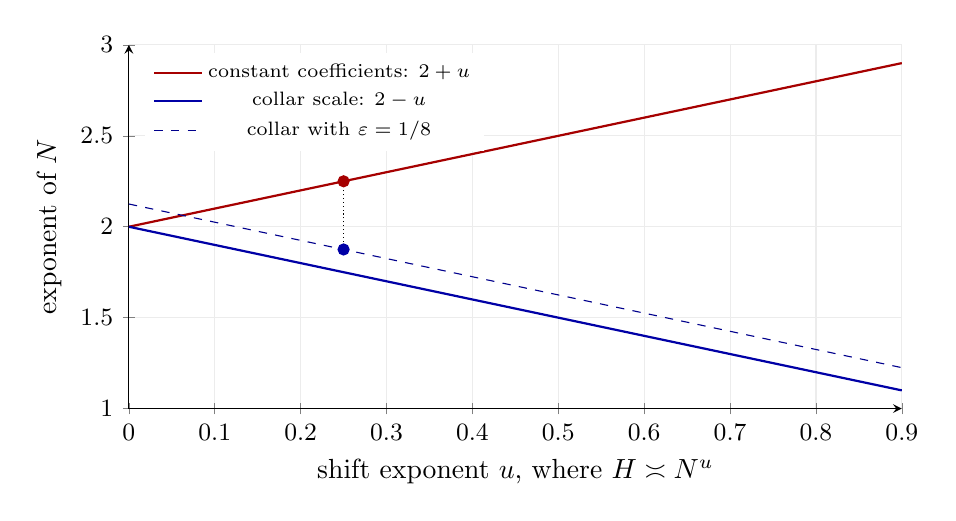
\begin{tikzpicture}
\begin{axis}[width=.94\linewidth,height=6.2cm,
 xmin=0,xmax=.9,ymin=1,ymax=3,
 xlabel={shift exponent \(u\), where \(H\asymp N^u\)},
 ylabel={exponent of \(N\)},grid=major,grid style={gray!15},
 axis lines=left,tick label style={font=\small},
 legend style={at={(.02,.98)},anchor=north west,draw=none,font=\scriptsize}]
\addplot[red!65!black,thick,domain=0:.9,samples=2]{2+x};
\addlegendentry{constant coefficients: \(2+u\)}
\addplot[blue!65!black,thick,domain=0:.9,samples=2]{2-x};
\addlegendentry{collar scale: \(2-u\)}
\addplot[blue!55!black,dashed,domain=0:.9,samples=2]{2.125-x};
\addlegendentry{collar with \(\varepsilon=1/8\)}
\addplot[only marks,mark=*,red!65!black] coordinates {(.25,2.25)};
\addplot[only marks,mark=*,blue!65!black] coordinates {(.25,1.875)};
\draw[densely dotted] (axis cs:.25,1.875)--(axis cs:.25,2.25);
\end{axis}
\end{tikzpicture}
\caption{The original exponent-gap comparison, with the
\(\varepsilon=1/8\) line made explicit. At \(u=1/4\) the marked
exponents are \(9/4\) and \(15/8\). For each fixed \(0<u<1\),
the exact maximum has exponent \(2+u\). The point \(u=1\) is
excluded: the block \(H=N\) contains no admissible shifts.}
\label{fig:v1-gap}
\end{figure}

\begin{lemma}[Square divisors and the signed correlation]
\label{lem:v1-square-divisor}
For every positive integer \(n\),
\[
 \lambda(n)=\sum_{r^2\mid n}\mu(n/r^2).
\]
Consequently, for integers \(Y\ge1\) and \(h\ge1\),
\begin{equation}\label{eq:v1-square-correlation}
 C_{\lambda,h}(Y)=
 \sum_{r\le\sqrt Y}\ \sum_{s\le\sqrt{Y+h}}
 \ \sum_{\substack{1\le n\le Y\\r^2\mid n,\ s^2\mid n+h}}
     \mu(n/r^2)\mu((n+h)/s^2).
\end{equation}
The inner sum is empty unless \(\gcd(r,s)^2\mid h\).
The summand indexed by \(r=s=1\) is exactly
\(\sum_{n\le Y}\mu(n)\mu(n+h)\).
\end{lemma}
\begin{proof}
Both sides of the first identity are multiplicative. At \(p^e\),
only \(e-2j=0\) or \(1\) contributes to
\(\sum_{2j\le e}\mu(p^{e-2j})\), giving \((-1)^e\).
Insert the identity into each factor of the correlation. All
sums are finite, so rearrangement is exact. The two congruences
\(n\equiv0\pmod{r^2}\), \(n\equiv-h\pmod{s^2}\) are compatible
exactly when \(\gcd(r^2,s^2)\mid h\), by the generalized Chinese
remainder theorem. This gcd is \(\gcd(r,s)^2\). The final
assertion follows by selecting \(r=s=1\).
\end{proof}

This identity preserves the multiplicative signs. The
\(r=s=1\) contribution is one stratum of the exact sum; it
does not approximate the whole correlation without an estimate
for the other strata. Replacing each M\"obius coefficient by its
absolute value would instead return to the coefficient-uniform
obstruction just proved.


\section{The maximal large sieve on a common support}\label{sec:sieve}

The maximal argument only needs a Bessel bound for all coefficient vectors on a single index set. We state it in that form. In the spectral application one uses the usual coefficient weights and the fixed-endpoint bound for the chosen spectrum, with the cutoff tied to the support of the coefficients. We make no shift-uniform assertion about short intervals placed at arbitrarily large indices.

\begin{theorem}[Maximal Bessel bound]\label{thm:bessel}
Let \((\Omega,\mu)\) be a positive measure space. Suppose \(\rho_1,\ldots,\rho_M\) satisfy
\[
 \int_{\Omega}\left|\sum_{n=1}^M b_n\rho_n\right|^2\dd\mu
 \le B\sum_{n=1}^M|b_n|^2
 \quad\text{for every }b\in\mathbb C^M.
\]
With \(K=\lceil\log_2 M\rceil\),
\[
 \int_{\Omega}\max_{0\le Y\le M}\left|\sum_{n\le Y}b_n\rho_n\right|^2\dd\mu
 \le (K+1)^2 B\sum_{n=1}^M|b_n|^2.
\]
\end{theorem}
\begin{proof}
Extend by zero to length \(2^K\). For each \(Y\), its prefix is the disjoint union of at most one aligned interval of each dyadic length. Cauchy--Schwarz bounds the square of its sum by \(K+1\) times the sum of the squared block sums. Enlarge to all aligned dyadic intervals and integrate. At each level the intervals partition the support, and the Bessel bound applies to each masked vector. The sum of the squared coefficient norms on that level is \(\sum_n|b_n|^2\). There are \(K+1\) levels.
\end{proof}

For example, take \(M=2N\) and coefficients supported on \(N<n\le2N\) in a spectral large sieve with fixed bound \(B\ll_\varepsilon (T^2+2N)(2TN)^\varepsilon\). The maximal bound has the same power exponents, since \((1+\log_2(2N))^2\) is absorbed by a smaller choice of \(\varepsilon\) in the fixed estimate. This is the Rademacher--Menshov argument applied to a spectral inequality of the Deshouillers--Iwaniec type \cite{di,rm}. It does not identify the coefficient vector needed for the signed Liouville problem.

\begin{proposition}[An additive Fourier benchmark]\label{prop:davenport}
For any \(a\) as above,
\[
 \E_a(N,H)\le (1+\lceil\log_2 N\rceil)^2
 \|A_N\|_{L^\infty(\mathbb R/\mathbb Z)}^2\sum_{n\le N}|a_n|^2.
\]
In particular Davenport's bound yields \(\E_\lambda(N,H)\ll_A N^3/(\log(2N))^A\) for every \(A>0\), uniformly in \(H\).
\end{proposition}
\begin{proof}
Extend \(a\one_{[1,N]}\) by zero to \(\mathbb Z\). For a dyadic block \(I\subset[1,2^{\lceil\log_2 N\rceil}]\), set \(a_I=a\one_I\). The Fourier transform of the full correlation \(\sum_n a_I(n)a(n+h)\) in \(h\) is \(A_N\overline{\widehat{a_I}}\), up to the Fourier sign convention. Parseval bounds its squared norm by \(\|A_N\|_\infty^2\sum_{n\in I}|a_n|^2\). Use the same dyadic decomposition as in Theorem~\ref{thm:bessel}, and sum over all integer \(h\) to majorize the chosen shifts. For the Liouville estimate apply Davenport's uniform additive bound in the form quoted in \cite{mrt}, with an increased logarithmic exponent.
\end{proof}

\section{Obstructions from signs and from prime data}\label{sec:obstructions}

We give two deterministic models with different properties and a probabilistic comparison. The first deterministic model retains the arithmetic data at any finite set of primes. The second retains the strength of the additive Fourier estimate that would follow from \eqref{eq:collar}.

\begin{theorem}[Finite prime data]\label{thm:prime}
For any finite set \(P\) of primes and signs \(\epsilon_p\) on \(P\), there exists a completely multiplicative sign function \(f\) with \(f(p)=\epsilon_p\) for \(p\in P\) and
\[
 \left|\sum_{n\le N} f(n)\right|\ll_P (1+\log N)^{|P\cup\{3\}|}.
\]
There is a positive integer \(D\) depending only on \(P\) such that
\(\E_f(N,H)\ge HN^2/(32D)\) whenever \(2D\le H\le N/4\).
\end{theorem}
\begin{proof}
Let \(S=P\cup\{3\}\) and let \(\chi_3\) be the nonprincipal character modulo \(3\). Specify the given values on \(P\), use \(f(3)=1\) if \(3\notin P\), and set \(f(p)=\chi_3(p)\) for \(p\notin S\). Extend completely multiplicatively. Write \(n=am\) with \(a\) supported on \(S\) and \((m,\prod_{p\in S}p)=1\). Then \(f(m)=\chi_3(m)\). The sum of \(\chi_3(m)\one_{(m,\prod_{p\in S}p)=1}\) over a complete residue system modulo \(\prod_{p\in S}p\) vanishes. The admissible residues with \(m\equiv1\) and \(m\equiv2\pmod 3\) have the same cardinality by the Chinese remainder theorem. Each inner sum over \(m\le N/a\) is therefore bounded by that period. There are at most \(\prod_{p\in S}(1+\lfloor\log N/\log p\rfloor)\) choices for \(a\).

Choose \(K\) with \(\sum_{p\in S}p^{-K}\le1/4\) and put \(D=\prod_{p\in S}p^K\). If \(D\mid h\) and \(p^K\nmid n\) for all \(p\in S\), then \(v_p(n+h)=v_p(n)\) for all \(p\in S\). The factor \(a\) is unchanged and \(h/a\) is divisible by \(3\). The two unit factors agree modulo \(3\), so \(f(n+h)=f(n)\). Among \(n\le Y\) the exceptional set has size at most \(Y/4\). Thus \(C_{f,h}(Y)\ge Y/2\) for \(D\mid h\). There are at least \(H/(2D)\) multiples of \(D\) in \((H,2H]\) under the stated conditions, and \(Y=N-h\ge N/2\) for those shifts. Squaring and summing gives the bound.
\end{proof}

\begin{theorem}[Additive cancellation and fixed shifts]\label{thm:rs}
There is a sign sequence \(r\) such that, with absolute constants,
\[
 \sup_\alpha\left|\sum_{n\le N}r_n\ee(n\alpha)\right|\ll\sqrt N,\qquad
 |C_{r,h}(Y)|\ll\sqrt{hY}\quad(h,Y\ge1).
\]
Nevertheless \(\E_r(3H,H)\ge H^2\) for every dyadic \(H\).
\end{theorem}
\begin{proof}
Use the Rudin--Shapiro polynomials \(P_0=Q_0=1\) and
\[
 P_{m+1}=P_m+z^{2^m}Q_m,\qquad Q_{m+1}=P_m-z^{2^m}Q_m.
\]
The prefixes of the \(P_m\) are consistent, and \(r_n=[z^{n-1}]P_m\) once \(n\le2^m\). The complementary identity
\(|P_m(z)|^2+|Q_m(z)|^2=2^{m+1}\) on \(|z|=1\)
follows by induction. Every aligned dyadic block of length \(2^j\) in the infinite sequence is the coefficient vector of \(\pm P_j\) or \(\pm Q_j\). This follows by taking recursive halves in a large enough \(P_m\). In the aligned dyadic partition of a prefix of length \(N\), each block contributes at most \(2^{(j+1)/2}\), and the sum over its lengths is \(O(\sqrt N)\).

If \(h>Y\), the fixed-shift estimate follows from the trivial bound \(Y\). Otherwise take \(B=2^k\) with \(\sqrt{hY}\le B<2\sqrt{hY}\). Partition the starting indices into full aligned blocks of length \(2B\) and a final remainder. Each full block consists of \(P_k\) and \(Q_k\), up to signs. The two sums for which both indices stay in the same half cancel by the \(h\)-th Fourier coefficient of the complementary identity. At most \(h\) starting indices cross the midpoint and at most \(h\) cross the endpoint of each block. The remainder contributes at most \(2B\). This bounds the sum by \(2h\lfloor Y/(2B)\rfloor+2B\ll\sqrt{hY}\).

Finally \(P_{m+2}\) has four successive blocks \(P_m,Q_m,P_m,-Q_m\). At \(H=2^m\), the first and third blocks give \(C_{r,2H}(H)=H\), an admissible endpoint for \(N=3H\). This one term already gives the lower bound.
\end{proof}

\begin{figure}[ht]
\centering
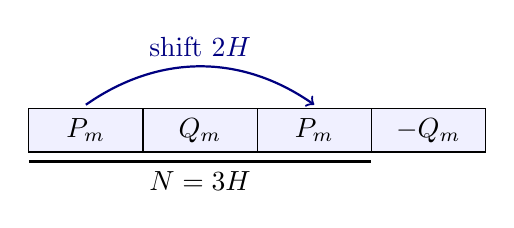
\begin{tikzpicture}[x=1.45cm,y=1cm]
\foreach \i/\t in {0/{P_m},1/{Q_m},2/{P_m},3/{-Q_m}} {
 \draw[fill=blue!6] (\i,0) rectangle ({\i+1},.55);
 \node at ({\i+.5},.275) {$\t$};
}
\draw[->,thick,blue!50!black] (.5,.6) to[bend left=35] node[above] {\(\text{shift }2H\)} (2.5,.6);
\draw[thick] (0,-.12)--(3,-.12);
\node[below] at (1.5,-.12) {\(N=3H\)};
\end{tikzpicture}
\caption{The first and third Rudin--Shapiro blocks agree entry by entry. Taking the endpoint \(Y=H\) sees this agreement before the fourth block can contribute.}
\label{fig:rs}
\end{figure}

\begin{proposition}[Independent signs]\label{prop:random}
For independent fair signs \(\epsilon_n\), almost surely \(\E_\epsilon(3H,H)\ge H^2/2\) for every sufficiently large dyadic \(H\).
\end{proposition}
\begin{proof}
Put \(T_H=\sum_{H<h\le2H}|C_{\epsilon,h}(H)|^2\). On expanding, the diagonal gives \(H^2\). The other terms are \(2\epsilon_n\epsilon_m\epsilon_{n+h}\epsilon_{m+h}\) with \(1\le n<m\le H\). Each set of four indices determines the term uniquely: the two indices in \([1,H]\) give \(n,m\), and the smaller remaining index gives \(n+h\). The products for distinct sets of indices are orthogonal in probability. Thus \(\mathbf E T_H=H^2\) and \(\operatorname{Var}(T_H)=4H\binom H2\le2H^3\). Chebyshev bounds the probability of \(T_H<H^2/2\) by \(8/H\). This is summable on the dyadic scales. Apply Borel--Cantelli and use \(\E_\epsilon(3H,H)\ge T_H\).
\end{proof}

\begin{proposition}[Random completely multiplicative signs]\label{prop:rmult}
Give the primes independent fair signs and extend them completely multiplicatively to \(f\). Then almost surely
\[
 \E_f(3H,H)\gg H^2/\log H
\]
for infinitely many dyadic \(H\).
\end{proposition}
\begin{proof}
Condition on all prime signs up to \(2H\). A composite integer at most \(3H\) has all prime factors at most \(3H/2\). Thus the only fresh signs in the vector \(C_{f,h}(H)\), \(H<h\le2H\), are those of primes \(p\in(2H,3H]\) in the second factor. Write the vector as \(u+\sum_p A_p\epsilon_p\), where \(u\) is fixed under the conditioning and \(A_p(h)=f(p-h)\) if \(1\le p-h\le H\), and zero otherwise. Let \(T=\sum_p\|A_p\|_2^2\). Each prime in \((2H,5H/2]\) contributes at least \(H/2\) nonzero coordinates for dyadic \(H\ge2\), so the prime number theorem gives \(T\gg H^2/\log H\).

For \(Z=\|u+\sum_p A_p\epsilon_p\|_2^2\), the conditional mean is \(m=\|u\|_2^2+T\). Orthogonality of the independent linear and quadratic sign monomials gives
\[
 \operatorname{Var}(Z)=4\sum_p|\langle u,A_p\rangle|^2+
 4\sum_{p<q}|\langle A_p,A_q\rangle|^2
 \le4\|u\|_2^2T+2T^2\le2m^2 .
\]
Since \(\mathbf E[Z\one_{Z\ge m/2}]\ge m/2\), Cauchy--Schwarz and \(\mathbf E[Z^2]\le3m^2\) give conditional probability at least \(1/12\) of \(Z\ge m/2\ge T/2\). All earlier dyadic events depend only on primes at most \(3H/2\), hence are measurable under the conditioning at scale \(H\). By iterative conditioning, the probability of no successes in any block of \(r\) consecutive large dyadic scales is at most \((11/12)^r\). Let \(r\to\infty\) and take the countable union over starting scales. The conclusion follows because \(\E_f(3H,H)\ge Z\).
\end{proof}

The complementary identities used in Theorem~\ref{thm:rs} belong to the classical Rudin--Shapiro construction. Peak aperiodic correlations of the full polynomials have a separate literature \cite{rs}. The prefix maximum in \(\E_a\) is essential to the block example.
\begin{theorem}[A deterministic logarithmic obstruction]\label{thm:gram-log}
For every sign sequence \(a\) and every \(B\ge0\), the number of dyadic \(H\) with
\[
 \E_a(3H,H)/H\le B
\]
is \(O(B+1)\), with an absolute constant. Consequently \(\E_a(3H,H)/H\to+\infty\) along all dyadic \(H\). In each range \(J/2\le j\le J\) of dyadic exponents, a positive proportion of the \(H=2^j\) satisfy \(\E_a(3H,H)\gg H\log H\), uniformly for sufficiently large \(J\).
\end{theorem}
\begin{proof}
Restrict first to one residue class of \(j\) modulo \(3\), so distinct scales increase by a factor of at least \(8\). Set \(M=\lceil64(B+1)\rceil\). Suppose there are \(K=2M\) scales \(H_i\ge M\), numbered in increasing order, with the stated bound. Put \(I_i=(3H_i/2,7H_i/4]\cap\mathbb Z\). Since \(H_i\) is divisible by \(4\), \(|I_i|=H_i/4\). For \(n\in I_i\) let \(v_n=(a_{n+1},\ldots,a_{n+M})^\mathsf{T}\) and form
\[
 B_i=|I_i|^{-1}\sum_{n\in I_i}v_nv_n^\mathsf{T}.
\]
These \(M\times M\) matrices are positive semidefinite with trace \(M\), so \(\operatorname{tr}(B_i^2)\le M^2\). For \(i<j\), \(n\in I_i\) and \(m\in I_j\), the gap \(h=m-n\) lies in \((H_j,2H_j]\), using \(H_i\le H_j/8\). Also \(m+M\le3H_j\). Thus
\[
 |v_n^\mathsf{T}v_m|=|C_{a,h}(n+M)-C_{a,h}(n)|
             \le2 C^*_{a,h}(3H_j).
\]
At a fixed \(h\) there are at most \(|I_i|\) pairs \((n,m)\). On expanding the cross trace this gives
\(\operatorname{tr}(B_iB_j)\le4\E_a(3H_j,H_j)/|I_j|\le16B\).
On the other hand, Cauchy--Schwarz on the \(M\) eigenvalues of \(\sum_i B_i\) gives \(\operatorname{tr}((\sum_i B_i)^2)\ge K^2 M\). The diagonal and cross bounds imply
\[
 K^2 M\le KM^2+16BK(K-1).
\]
With \(K=2M\), this forces \(M\le32B\), a contradiction.

There are therefore fewer than \(2M\) such scales above \(M\) in each residue class. The number of omitted smaller scales is \(O(1+\log M)\). This proves the bound on the number of exceptions. To obtain the last claim take \(B=cJ\) with a sufficiently small absolute \(c>0\), and apply the bound to the \(J/2+O(1)\) scales in the range.
\end{proof}

This argument applies to \(\lambda\) without a correlation theorem. It also proves that a fixed bound on the normalized collar cannot hold along any infinite sequence of dyadic scales for any sign sequence. The next result records an exact weighted second-moment asymptotic for the actual Liouville function.

\section{An endpoint obstruction for Liouville itself}\label{sec:tao}

The examples in Section~\ref{sec:obstructions} concern other sequences. To obtain a statement about \(\lambda\) itself we use Tao's logarithmically averaged two-point Chowla theorem \cite{tao}. We need only the consequence
\begin{equation}\label{eq:chowla}
 \sum_{t\le T}\frac{\lambda(t)\lambda(t+d)}{t}=o_d(\log T)
 \qquad(d\ge1\text{ fixed}).
\end{equation}

\begin{theorem}[Failure of the absolute endpoint]\label{thm:endpoint}
The Liouville collar satisfies
\[
 \lim_{J\to\infty}\frac1J
 \sum_{j=0}^{J-1}\frac{\E_\lambda(3\cdot 2^j,2^j)}{2^j}=+\infty.
\]
In particular, \(\E_\lambda(3H,H)/H\) is unbounded along dyadic \(H\).
\end{theorem}
\begin{proof}
Fix an integer \(M\ge1\). In
\[
 |C_{\lambda,h}(M)|^2=
 \sum_{1\le n,m\le M}\lambda(n)\lambda(m)\lambda(n+h)\lambda(m+h)
\]
the diagonal contributes \(M\). For \(n<m\), changing \(t=h+n\) changes the harmonic weights \(1/h\) to \(1/t\) with total error \(O_M(1)\), since \(\sum_{h\ge1}n/(h(h+n))<\infty\). Changing the endpoints costs \(O_M(1)\). By \eqref{eq:chowla}, the logarithmic mean of this off-diagonal term vanishes. The terms with \(m<n\) have the same treatment. Hence
\begin{equation}\label{eq:loggram}
 \sum_{h\le T}\frac{|C_{\lambda,h}(M)|^2}{h}
 =M\log T+o_M(\log T).
\end{equation}
When \(H\ge M\) and \(H<h\le2H\), the endpoint \(M\) is admissible at \(N=3H\), and \(1/h\le1/H\). Thus the contribution of that block to \eqref{eq:loggram} is at most \(\E_\lambda(3H,H)/H\). Sum over all dyadic \(H<2^J\), omitting the finitely many with \(H<M\) and the initial \(h=1\). After dividing by \(J\), the lower limit of the displayed average is at least \(M\log 2\). Since \(M\) was arbitrary, the limit is \(+\infty\).
\end{proof}

The theorem disproves the estimate with a fixed constant at exponent \(\varepsilon=0\). The argument takes \(M\) fixed before \(J\to\infty\) and supplies no positive power of \(H\). One can see the role of uniformity directly from the matrix in \eqref{eq:loggram}.

\begin{proposition}[A power saving in ordinary correlations would obstruct the collar]\label{prop:power}
Suppose there are \(\delta,\eta>0\) and \(K<\infty\) such that for all sufficiently large dyadic \(H\) and all \(1\le n<m\le H^\eta\),
\[
 \left|\sum_{H<h\le2H}\lambda(h+n)\lambda(h+m)\right|
 \le K H^{1-\delta}.
\]
For every \(0<\kappa<\min(\delta,\eta,1)\), one then has \(\E_\lambda(3H,H)\gg H^{1+\kappa}\) for large dyadic \(H\). Thus \eqref{eq:collar} would fail for \(\varepsilon<\kappa\).
\end{proposition}
\begin{proof}
Use \(M=\lfloor H^\kappa\rfloor\) and expand \(\sum_{H<h\le2H}|C_{\lambda,h}(M)|^2\). The diagonal is \(HM\), and the absolute value of the sum of off-diagonal terms is at most \(KM(M-1)H^{1-\delta}\). Its ratio to \(HM\) tends to zero. Use \(M\le H\) to bound the collar below by the resulting second moment.
\end{proof}

For comparison, ordinary two-point Chowla at every \emph{fixed} shift would imply
\(\E_\lambda(3H,H)/H\to\infty\) without Ces\`aro averaging. For fixed \(M\), the same expansion and subtraction of partial sums at \(H\) and \(2H\) give
\[
 \frac1H\sum_{H<h\le2H}|C_{\lambda,h}(M)|^2\to M .
\]
This conclusion uses the stated ordinary correlation input. The recent OpenAI manuscript \cite{oaichowla} gives fixed-affine-form estimates with logarithmic savings. Such savings do not supply the uniform power input in Proposition~\ref{prop:power}. Theorem~\ref{thm:endpoint} uses only the published logarithmic theorem \cite{tao}.

\section{A signed energy and its exact boundary terms}\label{sec:fejer}

Extend the truncation \(a_1,\ldots,a_N\) by zero to the integers, and write
\[
 S_{N,H}(t)=\sum_{t<n\le t+H}a_n\one_{[1,N]}(n),\quad
 \Q_a(N,H)=\frac1H\sum_{t\in\mathbb Z}|S_{N,H}(t)|^2.
\]
The sum over \(t\) has finite support. The factor \(H^{-1}\) normalizes the diagonal. Here \(H\ge1\) is any integer. We distinguish this \(H\), the window length, from a dyadic shift range in \(\E_a\).

\begin{proposition}[Fej\'er identity]\label{prop:fejer}
Let
\(F_H(\alpha)=H^{-1}|\sum_{j=1}^H\ee(j\alpha)|^2\).
Then
\begin{align}
 \Q_a(N,H)
 &=\int_0^1 |A_N(\alpha)|^2F_H(\alpha)\dd\alpha \label{eq:fejerfourier}\\
 &=\sum_{n\le N}a_n^2+
  2\sum_{h=1}^{\min(H-1,N-1)}(1-h/H) C_{a,h}(N-h).\label{eq:fejershift}
\end{align}
For \(L_a(j)=\sum_{n\le j}a_n\) one has
\begin{equation}\label{eq:fejerlower}
 \Q_a(N,H)\ge\frac{H}{N+H-1}|L_a(N)|^2 .
\end{equation}
If \(H\ge N\), one has the exact formula
\begin{align}
 \Q_a(N,H)
 &=\frac{H-N+1}{H}|L_a(N)|^2\nonumber\\
 &\quad+\frac1H\sum_{j=1}^{N-1}
  \bigl(|L_a(j)|^2+|L_a(N)-L_a(j)|^2\bigr). \label{eq:fejerboundary}
\end{align}
\end{proposition}
\begin{proof}
Two indices \(m,n\in[1,N]\) lie together in exactly \((H-|m-n|)_+\) integer windows, where \(u_+=\max(u,0)\). Expand the squares and group by \(m-n\). This gives \eqref{eq:fejershift}, and the same weights are the Fourier coefficients of \(F_H\), proving \eqref{eq:fejerfourier}. There are at most \(N+H-1\) windows meeting \([1,N]\). Each index lies in \(H\) windows, so \(\sum_t S_{N,H}(t)=H L_a(N)\). Cauchy--Schwarz proves \eqref{eq:fejerlower}. For \(H\ge N\), exactly \(H-N+1\) windows contain \([1,N]\), and each proper nonempty prefix and suffix occurs in one window. This gives \eqref{eq:fejerboundary}.
\end{proof}

At \(H=N\), let \(Q_a(N)=\Q_a(N,N)\). Completing the square in \eqref{eq:fejerboundary} gives
\begin{equation}\label{eq:completion}
 Q_a(N)=\frac{N+1}{2N}|L_a(N)|^2+
 \frac2N\sum_{j=1}^{N-1}|L_a(j)-\tfrac12 L_a(N)|^2.
\end{equation}
In particular, \(\tfrac12|L_a(N)|^2\le Q_a(N)\le
5\max_{j\le N}|L_a(j)|^2\), with the upper bound following directly from \eqref{eq:fejerboundary}. The two inequalities compare a single positive energy to the sum at its own endpoint and to the maximal prefix sum. They show why the square-root-scale Fej\'er question is neither an unsigned collar estimate nor a positivity statement alone.

\begin{figure}[ht]
\centering
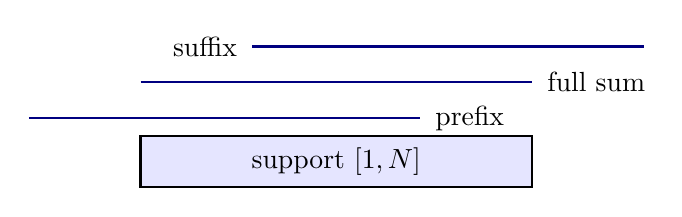
\begin{tikzpicture}[x=.71cm,y=.65cm]
\fill[blue!10] (1,0) rectangle (8,1);
\draw[thick] (1,0) rectangle (8,1);
\node at (4.5,.5) {support \([1,N]\)};
\draw[thick,blue!50!black] (-1,1.35)--(6,1.35);
\draw[thick,blue!50!black] (1,2.05)--(8,2.05);
\draw[thick,blue!50!black] (3,2.75)--(10,2.75);
\node[anchor=west] at (6.1,1.35) {prefix};
\node[anchor=west] at (8.1,2.05) {full sum};
\node[anchor=east] at (2.9,2.75) {suffix};
\end{tikzpicture}
\caption{Windows of length \(N\) in the zero-extended sequence. The boundary terms in \eqref{eq:fejerboundary} are exactly one copy of each proper prefix and suffix.}
\label{fig:windows}
\end{figure}

For independent fair signs, \(\mathbf E Q_\epsilon(N)=N\) by \eqref{eq:fejershift}, although the same model violates \eqref{eq:collar}. For alternating signs, \(Q_a(N)=1\) for every \(N\). When \(N\) is odd the full window contributes \(1\), and each proper prefix and its complementary suffix contribute \(1\) between them. When \(N\) is even the full window vanishes, and exactly \(N/2\) pairs of odd prefix and suffix contribute \(2\) each. For constant signs the boundary formula gives \(Q_{\mathbf 1}(N)=(N^2+2\sum_{j<N}j^2)/N=(2N^2+1)/3\). Thus alternating and constant signs have the same maximal absolute energy and different orders of signed energy.

\begin{figure}[ht]
\centering
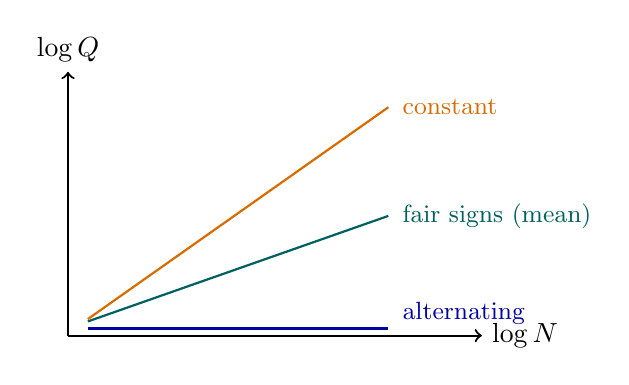
\begin{tikzpicture}[x=.72cm,y=1cm]
\draw[->,thick] (0,0)--(7.3,0) node[right] {\(\log N\)};
\draw[->,thick] (0,0)--(0,3.35) node[above] {\(\log Q\)};
\draw[thick,blue!65!black] (.35,.09)--(5.65,.09);
\draw[thick,teal!75!black] (.35,.18)--(5.65,1.52);
\draw[thick,orange!85!black] (.35,.21)--(5.65,2.9);
\node[anchor=west,font=\small,blue!65!black] at (5.73,.28) {alternating};
\node[anchor=west,font=\small,teal!75!black] at (5.73,1.52) {fair signs (mean)};
\node[anchor=west,font=\small,orange!85!black] at (5.73,2.9) {constant};
\end{tikzpicture}
\caption{Orders of the signed energy in the three models. The slopes are \(0,1,2\), respectively, from the exact formulas. The lines show the exponents schematically.}
\label{fig:energies}
\end{figure}

One may shorten the window at a known cost. If \(H=\lfloor N^\alpha\rfloor\) for \(0<\alpha\le1\) and \(\Q_\lambda(N,H)\ll_\varepsilon N^{1+\varepsilon}\), then \eqref{eq:fejerlower} implies \(L(N)\ll_\varepsilon N^{1-\alpha/2+\varepsilon}\). A sequence of such estimates with \(\alpha\) arbitrarily close to \(1\) would suffice for RH. Estimates confined to windows much shorter than \(N\) do not give that conclusion from this inequality.

\section{The zero-free exponent}\label{sec:zero}

We write \(Q_\lambda(N)=\Q_\lambda(N,N)\) and use \(\theta\) for a real number in \([1/2,1]\).

\begin{theorem}[Equivalent zero-free bounds]\label{thm:equiv}
The following conditions are equivalent.
\begin{enumerate}
\item \(\zeta(s)\ne0\) for \(\R s>\theta\).
\item \(L(x)\ll_{\theta,\varepsilon} x^{\theta+\varepsilon}\) for every \(\varepsilon>0\).
\item \(Q_\lambda(N)\ll_{\theta,\varepsilon} N^{2\theta+\varepsilon}\) for every \(\varepsilon>0\).
\end{enumerate}
In particular, the third condition at \(\theta=1/2\) is equivalent to RH.
\end{theorem}
\begin{proof}
The inequalities following \eqref{eq:completion} give the equivalence of the second and third conditions by rescaling \(\varepsilon\). For the implication from the second to the first, partial summation defines
\[
 F(s)=s\int_1^\infty L(x)x^{-s-1}\dd x
\]
holomorphically on \(\R s>\theta\). The convergence is locally uniform by taking \(\varepsilon\) smaller than the distance of a compact set from the boundary. For \(\R s>1\), \(F(s)=\sum_{n\ge1}\lambda(n)n^{-s}=\zeta(2s)/\zeta(s)\). This follows from the local factor \((1+p^{-s})^{-1}=(1-p^{-s})/(1-p^{-2s})\). The identity \(\zeta(s)F(s)=\zeta(2s)\) extends meromorphically. The right side has no zero on \(\R s>\theta\). This excludes a zero of the factor \(\zeta(s)\) there.

The reverse implication is classical. Appendix~\ref{sec:perron} supplies the reciprocal growth bound and the contour calculation with their dependence on the fixed distance from \(\R s=\theta\). At \(\theta=1\) the conclusion about \(L(x)\) is trivial. At \(\theta=1/2\), apply the functional equation to exclude nontrivial zeros to the left of the line.
\end{proof}

\begin{corollary}[Exact growth exponent]\label{cor:exponent}
Let \(\Theta\) be the supremum of the real parts of the nontrivial zeros of \(\zeta\). Then
\[
 \limsup_{N\to\infty}\frac{\log(1+Q_\lambda(N))}{\log N}=2\Theta .
\]
\end{corollary}
\begin{proof}
The functional equation and the existence of nontrivial zeros give \(1/2\le\Theta\le1\). Theorem~\ref{thm:equiv} at \(\theta=\Theta\) gives the upper bound. If \(\Theta>1/2\) and the limit superior were strictly smaller than \(2\Theta\), choose \(\theta\in[1/2,\Theta)\) strictly above half that limit superior. Theorem~\ref{thm:equiv} would exclude all zeros to the right of \(\theta\), contrary to the definition of \(\Theta\). If \(\Theta=1/2\) and the limit superior were less than \(1\), then \eqref{eq:completion} would give \(L(x)\ll x^\sigma\) with \(\sigma<1/2\). The Mellin integral would be holomorphic near \(1/2\), whereas the identity \(\zeta(s)F(s)=\zeta(2s)\) has a pole there on the right side and no pole on the left side. This is impossible.
\end{proof}

\begin{corollary}[A boundary constraint at the square-root scale]\label{cor:simple}
If \(Q_\lambda(N)\ll N(\log(2N))^B\) for some \(B\ge0\), then RH holds and every nontrivial zero has multiplicity at most \(1+B/2\). In particular, if \(B<2\) all nontrivial zeros are simple.
\end{corollary}
\begin{proof}
Theorem~\ref{thm:equiv} gives RH. The same bound and \eqref{eq:completion} give \(L(x)\ll x^{1/2}(\log(2x))^{B/2}\). At a nontrivial zero \(\rho=1/2+i\gamma\), the numerator \(\zeta(2\rho)\) is finite and nonzero by the classical nonvanishing on \(\R s=1\) and \(\gamma\ne0\). For \(u\downarrow0\), the Mellin integral at \(s=\rho+u\) is \(O_\rho(u^{-1-B/2})\) after the change of variable \(v=\log x\). A zero of multiplicity \(m\) gives a pole of order \(m\) in \(F\) at \(\rho\), which forces \(m\le1+B/2\).
\end{proof}

\subsection{Simultaneous pole contributions to the Fej\'er energy}
\label{ssec:fejer-multipole}

The signed Fej\'er energy also gives quantitative information at a
fixed exponent. The following bound records the contributions of any
finite set of poles on the same vertical line.

\begin{proposition}[A sum of pole contributions]\label{prop:fejer-multipole}
Put
\[
 M(s)=\frac{\zeta(2s)}{s\zeta(s)},\qquad
 K(s)=1+\frac{2}{1+2\R s}-2\R\frac1{1+s}.
\]
Fix \(\beta\ge1/2\) and an integer \(r\ge1\). For a finite set
\(\mathcal P\) of distinct poles \(\rho=\beta+i\gamma\) of \(M\)
of order exactly \(r\), write
\(A_\rho=\lim_{s\to\rho}(s-\rho)^rM(s)\). Then
\begin{equation}\label{eq:fejer-multipole}
 \limsup_{N\to\infty}
  \frac{Q_\lambda(N)}{N^{2\beta}(\log N)^{2r-2}}
 \ge \sum_{\rho\in\mathcal P}K(\rho)
              \left|\frac{A_\rho}{(r-1)!}\right|^2.
\end{equation}
If the limit superior is finite, \(M\) has no pole in
\(\R s>\beta\) and every pole on \(\R s=\beta\) has order at
most \(r\).
\end{proposition}

\begin{proof}
Take \(L(X)=0\) on \(0<X<1\). In the complex Hilbert space
\(\mathcal H=L^2((0,1);\mathbb C^2)\), put
\[
 U_X(u)=(L(uX),L(X)-L(uX)),\qquad w_s(u)=(u^s,1-u^s).
\]
For an integer \(N\), the value \(L(uN)=L(j)\) occupies the
interval \([j/N,(j+1)/N)\) for \(0\le j<N\). By
\eqref{eq:fejerboundary}, this gives
\(\|U_N\|_{\mathcal H}^2=Q_\lambda(N)\). For \(X=N+a\),
\(0\le a<1\), the substitution \(v=uX\) gives the exact
interpolation
\begin{equation}\label{eq:fejer-norm-interpolation}
 \|U_X\|_{\mathcal H}^2
   =\frac{NQ_\lambda(N)+a|L(N)|^2}{X}.
\end{equation}
Since \(|L(N)|^2\le2Q_\lambda(N)\) by \eqref{eq:completion},
the numerator in \eqref{eq:fejer-multipole} can be replaced by
\(\|U_X\|_{\mathcal H}^2\) and the limit superior taken over
real \(X\), with the denominator at \(X\). Denote the resulting
limit superior by \(C\).

For \(\R s>1\), \(\|U_X\|_{\mathcal H}\ll X\) ensures absolute
convergence of the Hilbert space integral
\begin{equation}\label{eq:fejer-vector-mellin}
 \int_1^\infty U_X X^{-s}\frac{\dd X}{X}=M(s)w_s.
\end{equation}
For the first coordinate, substitute \(v=uX\), and use
\(L(v)=0\) below~1. For the second, subtract the first coordinate
from the transform of \(L(X)\). The scalar transform of \(L\) is
\(M(s)\) by partial summation and the Euler product. The map
\(s\mapsto w_s\) is holomorphic into \(\mathcal H\) on
\(\R s>-1/2\), since on compact subsets the derivatives of
\(u^s\) are dominated in \(L^2\) by a power of \(u\) times a
power of \(|\log u|\). Direct integration gives
\(\|w_s\|_{\mathcal H}^2=K(s)>0\) there.

If \(C=\infty\), \eqref{eq:fejer-multipole} is immediate.
Otherwise put \(F(t)=e^{-\beta t}U_{e^t}\) for \(t\ge0\).
The definition of \(C\) gives
\(\|F(t)\|_{\mathcal H}\ll 1+t^{r-1}\).
Consequently the integral in \eqref{eq:fejer-vector-mellin}
is holomorphic for \(\R s>\beta\). Meromorphic continuation
identifies it with the displayed right side there. As
\(w_s\ne0\), this excludes poles of \(M\) in that open
half-plane. At a boundary point \(\rho\), the same bound on
\(F\) gives \(\|M(\rho+\delta)w_{\rho+\delta}\|_{\mathcal H}
=O(\delta^{-r})\) as \(\delta\downarrow0\), which excludes
a pole of order greater than \(r\).

For each \(\delta>0\), equip the space of \(\mathcal H\)-valued
functions on \([0,\infty)\) with the \(L^2\) norm for the
measure \(e^{-\delta t}\dd t\). Denote its inner product by
\(\langle\cdot,\cdot\rangle_\delta\), linear in its first
argument, and put \(G_r=\Gamma(2r-1)\). For every
\(\varepsilon>0\), the bound
\(\|F(t)\|_{\mathcal H}^2\le(C+\varepsilon)t^{2r-2}\) holds
for all sufficiently large \(t\). Its integral over a fixed
bounded interval remains bounded as \(\delta\downarrow0\).
Thus Euler's gamma integral gives
\begin{equation}\label{eq:fejer-multipole-abel}
 \limsup_{\delta\downarrow0}\delta^{2r-1}\|F\|_\delta^2
 \le C G_r.
\end{equation}

For each \(\rho=\beta+i\gamma\in\mathcal P\), take the test
function
\[
 g_{\rho,\delta}(t)=\frac{\delta^{r-1/2}}{\sqrt{G_r}}
    t^{r-1} e^{i\gamma t}\,v_\rho,
 \qquad v_\rho=\frac{w_\rho}{\|w_\rho\|_{\mathcal H}}.
\]
Its norm is one. For \(\rho\ne\rho'\), the magnitude of
\(\langle g_{\rho,\delta},g_{\rho',\delta}\rangle_\delta\)
is at most
\((\delta/|\delta-i(\gamma-\gamma')|)^{2r-1}\), again by
the gamma integral. Hence the largest eigenvalue of this finite
Gram matrix tends to one. By \eqref{eq:fejer-vector-mellin},
\[
 \langle F,g_{\rho,\delta}\rangle_\delta
  =\frac{\delta^{r-1/2}}{\sqrt{G_r}}
  \left\langle
   (-1)^{r-1}\frac{\dd^{r-1}}{\dd s^{r-1}}
           [M(s)w_s]\bigg|_{s=\rho+\delta},v_\rho
  \right\rangle_{\mathcal H}.
\]
The signed derivative of the leading Laurent term
\(A_\rho w_\rho(s-\rho)^{-r}\) is
\[G_r A_\rho w_\rho(s-\rho)^{-(2r-1)}/(r-1)!.\]
Consequently
\[
 \lim_{\delta\downarrow0}\delta^{r-1/2}
       \langle F,g_{\rho,\delta}\rangle_\delta
   =\sqrt{G_r}\,\frac{A_\rho}{(r-1)!}\|w_\rho\|_{\mathcal H}.
\]
The sum of the squared scalar products with the tests is at
most \(\|F\|_\delta^2\) times their largest Gram eigenvalue.
Indeed the operator sending coordinate vectors to the tests
has squared norm equal to that eigenvalue, and the analysis
map taking scalar products is its adjoint. Multiply by
\(\delta^{2r-1}\), let \(\delta\downarrow0\) using
\eqref{eq:fejer-multipole-abel}, and divide by \(G_r\).
This proves \eqref{eq:fejer-multipole}.
\end{proof}

\begin{corollary}[A critical-line lower bound]\label{cor:fejer-critical-poles}
For every finite set \(\mathcal Z\) of simple critical-line
zeros of \(\zeta\),
\begin{equation}\label{eq:fejer-critical-poles}
 \limsup_{N\to\infty}\frac{Q_\lambda(N)}N
 \ge\frac{2}{3|\zeta(1/2)|^2}
 +\sum_{\rho\in\mathcal Z}
   \left(2-2\R\frac1{1+\rho}\right)
   \left|\frac{\zeta(2\rho)}{\rho\zeta'(\rho)}\right|^2.
\end{equation}
The left side is infinite if RH fails or if any critical-line
zero has multiplicity greater than one.
\end{corollary}

\begin{proof}
At \(s=1/2\) the residue of \(M\) is \(1/\zeta(1/2)\),
and \(K(1/2)=2/3\). At a simple critical zero \(\rho\), its
residue is \(\zeta(2\rho)/(\rho\zeta'(\rho))\). The numerator
is nonzero by the classical nonvanishing of \(\zeta\) on
\(\R s=1\). Apply Proposition~\ref{prop:fejer-multipole} with
\(\beta=1/2\), \(r=1\) and \(\mathcal P=\{1/2\}\cup\mathcal Z\).
Any right-hand zero, or critical zero of higher multiplicity,
would give an excluded pole in the case of a finite limit
superior. The functional equation reflects any off-line zero
to the right of the critical line if necessary.
\end{proof}

The verified simple zeros of \cite{pt} give strictly positive
terms in \eqref{eq:fejer-critical-poles}. Each finite set of
such zeros gives a lower bound, and adding further zeros
increases it. The estimate concerns the lower side of the
energy question. The square-root-scale upper bound with an
arbitrary power loss remains open.

\paragraph{Two certified numerical lower bounds.}
Using the first \(1000\) positive simple critical zeros and their
conjugates in \eqref{eq:fejer-critical-poles} gives a right side
strictly above \(45769/100000\). The calculation uses
outward-rounded ball arithmetic at \(128\) bits. The supplied
verification script isolates the zeros, checks that the ordinate
enclosures are disjoint, and encloses the derivative and residue
at each zero. The \texttt{python-flint}~0.9.0 interface calls
the rigorous FLINT zeta routines described in its
\href{https://flintlib.org/doc/acb_dirichlet/index.html\#zeros-of-the-riemann-zeta-function}%
{documentation}. No zero outside the stated set enters the sum.

A positive weighting in the logarithmic variable yields
the stronger certified bound
\begin{equation}\label{eq:fejer-weight-bound}
 \limsup_{N\to\infty}\frac{Q_\lambda(N)}{N}
 >\frac{3257}{5000}=0.6514.
\end{equation}
To prove it, let \(C\) denote the limit superior in
\eqref{eq:fejer-weight-bound}. If \(C<\infty\), the proof of
Proposition~\ref{prop:fejer-multipole} gives, for
\(F(t)=e^{-t/2}U_{e^t}\),
\(\limsup_{t\to\infty}\|F(t)\|_{\mathcal H}=\sqrt C\).
Let \(\rho_1=1/2+i\gamma_1\) be the first positive critical zero,
\(A_1=\zeta(2\rho_1)/(\rho_1\zeta'(\rho_1))\), and
\(a=-1/\zeta(1/2)>0\). For \(m=100\), put
\[
 P(t)=\frac{1}{m+1}
     \left|\sum_{j=0}^{m}e^{ij(\gamma_1t-\theta)}\right|^2,
 \qquad e^{i\theta}A_1=-|A_1|.
\]
The trigonometric polynomial is nonnegative and its constant
coefficient is one, so
\(\delta\int_0^\infty e^{-\delta t}P(t)\dd t\to1\).
For each \(\varepsilon>0\), the norm of \(F(t)\) is at most
\(\sqrt C+\varepsilon\) outside a fixed bounded interval. The
integral on that interval vanishes after multiplication by
\(\delta\). Thus the limit of
\(\delta\int_0^\infty e^{-\delta t}P(t)F(t)\dd t\), when it
exists, has norm at most \(\sqrt C\).

For \(2\le k\le100\), ball arithmetic verifies
\(\zeta(1/2+ik\gamma_1)\ne0\) by enclosing its value over the
whole ordinate enclosure. Equation~\eqref{eq:fejer-vector-mellin}
then shows that the terms at those frequencies and their
conjugates vanish in the limit. The constant term contributes
\(-a w_{1/2}\). The two terms at frequencies \(\pm\gamma_1\)
give \(-c\R w_{\rho_1}\) with
\(c=2m|A_1|/(m+1)\), since the first Fourier coefficient of
\(P\) has modulus \(m/(m+1)\). The limit therefore exists and
\[
 C\ge \|a w_{1/2}+c\R w_{\rho_1}\|_{\mathcal H}^2.
\]
Writing \(v=\R w_{\rho_1}\), direct integration gives
\begin{align*}
 \|w_{1/2}\|_{\mathcal H}^2&=\frac23,\\
 \|v\|_{\mathcal H}^2&=\frac32+\R\frac1{1+2\rho_1}
                       -2\R\frac1{1+\rho_1},\\
 \langle w_{1/2},v\rangle_{\mathcal H}
    &=\frac13-\R\frac1{1+\rho_1}+2\R\frac1{3/2+\rho_1}.
\end{align*}
The same script encloses the squared norm and verifies that
its lower endpoint exceeds the exact rational \(3257/5000\).
This proves \eqref{eq:fejer-weight-bound}, including the
immediate case \(C=\infty\).


\section{What the recent results give}\label{sec:frontier}

The recent advances concern different quantities. Anthropic's result controls a lower proportion of simple zeros on the critical line through Weil's form and pair correlation \cite{anthropic}. Lamzouri's independent proof obtains more than \(67.25\%\) of zeros that are both simple and on the line \cite{lamzouri}. Guth and Maynard's large-value estimates bound the number of zeros to the right of a specified line as a function of height \cite{gm}. A count of this type can allow an exceptional zero. Corollary~\ref{cor:exponent} shows that even one such zero affects the energy exponent. A rigorous computation of Platt and Trudgian checks all positive ordinates through \(3\cdot10^{12}\) \cite{pt}. The height cutoff, the proportion and the horizontal threshold are separate quantities.

The OpenAI quasi-Riemann manuscript states that \(\zeta(s)\ne0\) for \(\R s>7/8\), with a Lean formalization of the stated zero-free result in the accompanying repository \cite{oai,oaiscope}. Taking this zero-free statement as input in Theorem~\ref{thm:equiv} gives
\[
 L(x)\ll_\varepsilon x^{7/8+\varepsilon},
 \qquad Q_\lambda(N)\ll_\varepsilon N^{7/4+\varepsilon}.
\]
The difference between \(7/4\) and \(1\) is precisely the remaining power in this application. The quasi-Riemann input is used only for this specialization, and the proofs of the energy identities, the equivalence, the counterexamples and the endpoint obstruction do not use it.

The proof attempt in this revision proceeds by retaining the signs through \eqref{eq:fejershift}. At \(H=N\), the desired estimate is exactly an upper bound \(O_\varepsilon(N^{1+\varepsilon})\) for the diagonal \(N\) plus the weighted signed correlation sum. The termwise absolute-value route would require control of a different quantity, and Sections~\ref{sec:obstructions} and \ref{sec:tao} show why naive random-sign or fixed-shift estimates do not provide it. Additive Fourier cancellation controls the energy through \eqref{eq:fejerfourier}, but an \(O(N^{1/2+\varepsilon})\) uniform Fourier bound already includes the estimate for \(L(N)\) at \(\alpha=0\). Using it as an input would therefore assume the required strength. The remaining estimate is the signed energy bound itself, or another estimate that excludes all zeros with \(1/2<\R s\le7/8\) when the quasi-Riemann input is used.

\subsection{Refinements after the seven-eighths manuscript}

Liu's revised arXiv preprint \cite{liu1} reports the threshold
\begin{align*}
 b_1&=\frac{18\xi+7}{18\xi+9}=0.874957019420098946\ldots,\\
 0&=1188\xi^3-2160\xi^2+171\xi+190,
\end{align*}
with \(\xi\in(0.38858,0.38859)\). A later preprint \cite{liu2} reports a general-number-field threshold \(b_2=0.874886647039964\ldots\), specified by a quartic equation. The version 3 PDF of \cite{liu3}, Theorem 1.1, reports
\[
 b_{\rm tw}=0.87405850379185900499\ldots
\]
for all finite-order Hecke \(L\)-functions over all number fields, by a further unit-twisted comparison. These are external research preprints. The conditional specializations below use their stated zero-free theorems, whose full analytic proofs are not reproduced or independently verified in this revision.

For any of these thresholds \(b\), taking the corresponding zero-free statement as input in Theorem~\ref{thm:equiv} and Proposition~\ref{prop:smoothed} gives
\[
 L(x)\ll_\varepsilon x^{b+\varepsilon},\qquad
 B(X)\ll_\varepsilon X^{b+\varepsilon},\qquad
 Q_\lambda(N)\ll_\varepsilon N^{2b+\varepsilon}.
\]
The same input for all Dirichlet characters specializes Theorem~\ref{thm:char-grh}. These deductions follow directly from the proved transfer criteria, and are attributed to their zero-free input.

The comparison in \cite{liu3}, Section 25, improves a starting boundary through a recurrence \(b_{j+1}=b_{\rm tw}+(b_j-b_{\rm tw})/50\). Its exact solution is \(b_j=b_{\rm tw}+(b_0-b_{\rm tw})/50^j\), by induction. Thus that iteration converges to \(b_{\rm tw}\). Section 27 gives a limitation for its stated comparison system even under an improved width input. Neither calculation gives an iteration to \(1/2\).

\section{Proof attempts without Chowla}\label{sec:bypass}

The logarithmic correlation theorem was used for the obstruction in Section~\ref{sec:tao}. The two constructions below use only one-variable Dirichlet series and Mellin transforms. They give different sufficient estimates for RH.

\subsection{A single smooth weight that detects every right-hand zero}

Let \(B(X)=\sum_{n\ge1}\lambda(n)e^{-n/X}\) for \(X>0\). This sum is absolutely convergent. For \(\R s>1\), absolute convergence and the substitution \(y=n/X\) give
\begin{equation}\label{eq:gamma}
 \int_0^\infty B(X)X^{-s}\frac{\dd X}{X}
 =\Gamma(s)\frac{\zeta(2s)}{\zeta(s)}.
\end{equation}
The integral over \(0<X\le1\) is entire because \(|B(X)|\le e^{-1/X}/(1-e^{-1/X})\).

\begin{proposition}[A smoothed bypass]\label{prop:smoothed}
For \(1/2\le\theta\le1\), the bound \(B(X)\ll_{\varepsilon,\theta}X^{\theta+\varepsilon}\) for all \(\varepsilon>0\) is equivalent to the zero-free condition \(\zeta(s)\ne0\) for \(\R s>\theta\).
\end{proposition}
\begin{proof}
Under the bound, the integral in \eqref{eq:gamma} is holomorphic on \(\R s>\theta\). The identity extends meromorphically, and neither \(\Gamma(s)\) nor \(\zeta(2s)\) vanishes there. For the converse use Theorem~\ref{thm:equiv} and the partial summation identity
\(
 B(X)=X^{-1}\int_1^\infty L(u)e^{-u/X}\dd u.
\)
Changing \(u=Xv\) gives the required bound for \(X\ge1\).
\end{proof}

The nonvanishing of the Mellin weight in \eqref{eq:gamma} matters. In the recent work of Li, Sun and Wang \cite{lsw}, a particularly effective weight is built from \(W(x)=\sum_{m\ge1}V(mx)\), where \(V\) is smooth, compactly supported in \((0,\infty)\), and \(\int_0^\infty V=0\). At each \(X>0\) the sums below are finite. Complete multiplicativity gives
\[
 \sum_{n\ge1}\lambda(n)W(n/X)=
 \sum_{r\ge1}V(r/X)\sum_{n\mid r}\lambda(n)
 =\sum_{j\ge1}V(j^2/X).
\]
Indeed \(\sum_{k=0}^\ell (-1)^k\) is \(1\) when \(\ell\) is even and \(0\) otherwise, which proves the divisor identity prime by prime. The sum on the right is \(O_V(\sqrt X)\) for \(X\ge1\), by the support of \(V\). For \(\R s>1\), however, the Mellin transform of \(W\) is \(\zeta(s)\widehat V(s)\), where \(\widehat V(s)=\int_0^\infty V(x)x^{s-1}\dd x\). The equality continues to the right half-plane by Poisson summation. To see the convergence at zero, extend \(V\) by zero to \(\mathbb R\) and write \(\sum_{m\in\mathbb Z}V(mx)=x^{-1}\sum_{k\in\mathbb Z}\widehat V_{\mathrm F}(k/x)\), with \(\widehat V_{\mathrm F}\) the Fourier transform. The \(k=0\) term vanishes and the others decay faster than any fixed power as \(x\downarrow0\). The factor \(\zeta(s)\) cancels the very poles that the Mellin test needs to detect.\footnote{Li, Sun and Wang also construct a different weight adapted to a specified zero in their Appendix A. The pole cancellation here concerns the divisor-convolution weight only.}

\subsection{Reciprocal dilates with an explicit error rate}

The Nyman--Beurling criterion and its discrete strengthening \cite{baez,burnol} suggest working with reciprocal dilates. For \(n\ge1\), define the balanced functions
\[
 g_n(x)=\{1/(nx)\}-n^{-1}\{1/x\},\qquad x>0.
\]
They vanish for \(x>1\). For \(1/2\le\sigma<1\), set
\[
 \|u\|_\sigma^2=\int_0^1 |u(x)|^2 x^{2\sigma-1}\dd x,\qquad
 d_{M,\sigma}=\inf_{c_1,\ldots,c_M\in\mathbb C}
      \left\|1-\sum_{n\le M}c_ng_n\right\|_\sigma.
\]
The norm at \(\sigma=1/2\) is the ordinary \(L^2(0,1)\) norm. The functions \(\{nx\}\) considered in \cite{nbdraft} form a different approximation problem. Appendix~\ref{sec:ordinary} solves that finite problem and explains the difference.

\begin{lemma}[Exact Mellin transform]\label{lem:nbmellin}
For \(0<\R s<1\),
\[
 \int_0^1 g_n(x)x^{s-1}\dd x
 =-(n^{-s}-n^{-1})\frac{\zeta(s)}{s}.
\]
\end{lemma}
\begin{proof}
After substituting \(y=1/(nx)\) in the integral of the unbalanced function over \(x>0\), the transform is \(n^{-s}\int_0^\infty\{y\}y^{-s-1}\dd y\). On \(0<y<1\) the integral is \(1/(1-s)\). On \(y>1\) it is \(1/(s-1)-\zeta(s)/s\) by the Euler summation identity in Appendix~\ref{sec:perron}. The two rational terms cancel. Subtract the corresponding \(n^{-1}\) multiple of the \(n=1\) transform and use the support of \(g_n\).
\end{proof}

\begin{theorem}[Convergence in shifted norms]\label{thm:shifted}
Suppose \(1/2\le\theta<\sigma<1\) and \(\zeta\) has no zero in \(\R s>\theta\). For each \(0<\delta<\sigma-\theta\), the explicit choice
\[
 c_n=-\mu(n)(1-n/M)\qquad (n\le M)
\]
satisfies \(\|1-\sum_{n\le M}c_ng_n\|_\sigma\ll_{\sigma,\theta,\delta}M^{-\delta}\). Conversely, for every nontrivial zero \(\rho\) with \(\R\rho>\sigma\),
\[
 d_{M,\sigma}^2\ge \frac{2(\R\rho-\sigma)}{|\rho|^2}
 \quad\text{for every }M .
\]
\end{theorem}
\begin{proof}
Let \(D_M(s)=\sum_{n\le M}\mu(n)(1-n/M)n^{-s}\). For \(s=\sigma+it\), absolute convergence on \(\R w=2\) gives
\[
 D_M(s)=\frac1{2\pi i}\int_{\R w=2}
        \frac{M^w}{w(w+1)\zeta(s+w)}\dd w .
\]
The scalar kernel identity follows by closing left when \(M/n>1\), with residues \(1\) and \(-n/M\), and closing right when \(M/n<1\). At \(n=M\) the kernel is zero by continuity, using absolute convergence on \(\R w=2\).

Move the contour to \(\R w=-\delta\). There is only the residue \(1/\zeta(s)\) at \(w=0\). There are no poles from zeros because \(\sigma-\delta>\theta\), and \(-\delta>-1\). Lemma~\ref{lem:subpower} and the Euler product to its right show that the horizontal integrals tend to zero for each fixed \(t\). On the new vertical line the integral is
\[
 O_{\sigma,\theta,\delta,\eta}
 \left(M^{-\delta}\int_{\mathbb R}
 \frac{(1+|t+v|)^\eta}{(1+|v|)^2}\dd v\right)
 =O_{\sigma,\theta,\delta,\eta}(M^{-\delta}(1+|t|)^\eta)
\]
for \(0<\eta<1\). The last equality follows from \(1+|t+v|\le(1+|t|)(1+|v|)\). The same argument at \(s=1\) gives \(D_M(1)=O(M^{-\delta})\) because \(1/\zeta(1)=0\) in the removable extension.

By Lemma~\ref{lem:nbmellin}, the residual has Mellin transform \([1-\zeta(s)(D_M(s)-D_M(1))]/s\). The proof of Lemma~\ref{lem:subpower} bounds \(|\zeta(s)|\) by \(O((1+|t|)^\eta)\) on \(\R s=\sigma\) as well, using \(+\R G\) instead of \(-\R G\). Thus the residual transform is \(O(M^{-\delta}(1+|t|)^{2\eta-1})\). For \(\eta<1/4\) its square integrates. Apply Plancherel to \(e^{-\sigma y}u(e^{-y})\one_{y>0}\) with \(y=-\log x\). Its squared norm is \(\|u\|_\sigma^2\), and its Fourier transform in angular frequency is the Mellin transform on \(\R s=\sigma\). This proves the upper bound.

If \(\R\rho>\sigma\), the residual evaluates to \(1/\rho\) at \(\rho\). Cauchy--Schwarz in the weighted space bounds the absolute value of the evaluation by \(\|u\|_\sigma(2(\R\rho-\sigma))^{-1/2}\). This proves the lower bound uniformly in the coefficients.
\end{proof}

Taking the published quasi-Riemann manuscript as input gives convergence for \(\sigma>7/8\). The proof loses its positive choice of \(\delta\) as \(\sigma\downarrow7/8\). For a proof of RH, it would suffice to find any sequence of balanced reciprocal-dilate polynomials for which the residual tends to zero at \(\sigma=1/2\), by the lower bound in Theorem~\ref{thm:shifted} and the functional equation.\footnote{A boundary point on \(\R s=\sigma\) is not a bounded evaluation in the weighted Hilbert space. The argument for a hypothetical zero strictly to the right therefore gives no pointwise evaluation bound on the line itself.} The explicit construction proves the convergence away from the zero-free boundary. It leaves the critical norm unbounded by a quantity tending to zero.

One can quantify the cost of trying to reach the critical norm by interpolation. For \(0<\sigma_0<1/2<\sigma_1<1\), H\"older's inequality gives
\[
 \|u\|_{1/2}\le \|u\|_{\sigma_0}^{1-t}\|u\|_{\sigma_1}^{t},
 \qquad t=\frac{1/2-\sigma_0}{\sigma_1-\sigma_0}.
\]
For the explicit residual \(u_M=1-\sum c_ng_n\), the trivial coefficient bound gives \(\|u_M\|_{\sigma_0}\ll_{\sigma_0}M^{1-\sigma_0}\). Indeed, write \(x=1/y\). For \(n\le y\), \(|g_n(1/y)|\le 2\), and for \(n>y\), \(|g_n(1/y)|=\lfloor y\rfloor/n\). Consequently \(|u_M(1/y)|\ll y(1+\log(M/y))\) when \(1\le y\le M\), and \(|u_M(1/y)|\ll M\) otherwise. Integrating the square with weight \(y^{-2\sigma_0-1}\) gives the stated bound, using \(y=Mv\) in the first integral. Even with \(\delta\) at its limiting value \(\sigma_1-\theta\), the numerator of the interpolated exponent is
\[
 (\sigma_1-\tfrac12)(1-\sigma_0)
  -(\tfrac12-\sigma_0)(\sigma_1-\theta)
 =\tfrac12(\sigma_1-\tfrac12)+(\tfrac12-\sigma_0)(\theta-\tfrac12)>0 .
\]
Thus this interpolation with the available lower-norm estimate cannot prove decay at \(1/2\).

\begin{figure}[ht]
\centering
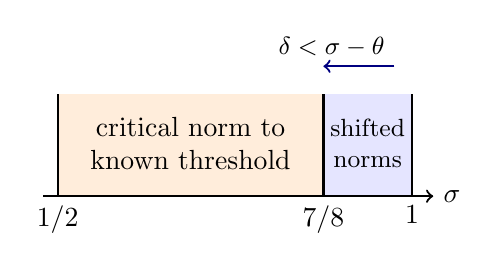
\begin{tikzpicture}[x=9cm,y=1cm]
\fill[orange!14] (.5,0) rectangle (.875,1.3);
\fill[blue!10] (.875,0) rectangle (1,1.3);
\draw[->,thick] (.48,0)--(1.03,0) node[right] {\(\sigma\)};
\foreach \x/\t in {.5/{1/2},.875/{7/8},1/{1}} {
 \draw[thick] (\x,0)--(\x,1.3);
 \node[below] at (\x,0) {\(\t\)};
}
\node[align=center] at (.6875,.67) {critical norm to\\known threshold};
\node[align=center,font=\small] at (.9375,.67) {shifted\\norms};
\draw[->,thick,blue!50!black] (.975,1.65)--(.875,1.65);
\node[anchor=south east,font=\small] at (.975,1.65) {\(\delta<\sigma-\theta\)};
\end{tikzpicture}
\caption{The shifted-norm construction with the \(7/8\) input. The rate in Theorem~\ref{thm:shifted} depends on the distance to the right of the zero-free boundary.}
\label{fig:strip}
\end{figure}

\subsection{Why the explicit family stops at the critical norm}

The failed interpolation does not settle whether the same coefficients might converge by a different argument. The following rescaling calculation answers that question. The obstruction is present even if all zeta zeros lie on the line. For related failures of natural approximants, see B\'aez-Duarte \cite{bd-arith}.

\begin{theorem}[A critical-norm obstruction for the linear Riesz family]\label{thm:riesz-failure}
For \(M\ge2\) let
\[
 u_M(x)=1+\sum_{n\le M}\mu(n)(1-n/M)g_n(x).
\]
Then \(\limsup_{M\to\infty}\|u_M\|_{1/2}>0\). The infimum over coefficients defining \(d_{M,1/2}\) is a separate problem.
\end{theorem}
\begin{proof}
Put \(b_m=\sum_{n\mid m}n\mu(n)=\prod_{p\mid m}(1-p)\) and \(B_1(y)=\sum_{m\le y}b_m\). For \(1\le y\le M\),
\begin{equation}\label{eq:riesz-rescale}
 u_M(1/y)=\lfloor y\rfloor D_M(1)+M^{-1}B_1(y).
\end{equation}
Indeed \(g_n(1/y)=\lfloor y\rfloor/n-\lfloor y/n\rfloor\). In the second term the unweighted sum \(\sum_{n\le M}\mu(n)\lfloor y/n\rfloor\) equals \(1\), by the divisor identity \(\sum_{n\mid m}\mu(n)=\one_{m=1}\). The remaining weighted sum is \(B_1(y)/M\). Formula \eqref{eq:riesz-rescale} holds for real \(M\) as well as integers.

Suppose that \(\|u_M\|_{1/2}\to0\) along the integers. The same would hold for real \(M\). To see this, put \(m=\lfloor M\rfloor\). Only the coefficients at \(n\le m\) contribute to the difference, and their differences have absolute value at most \(n/m^2\). As \(|g_n|\le2\), the differences of the functions are uniformly bounded. At fixed \(x=1/y\in(0,1)\), for \(n>y\) one has \(g_n(x)=\lfloor y\rfloor/n\), so the difference tends to zero pointwise. Dominated convergence gives the claim.

Choose a nontrivial zero \(\rho=1/2+i\gamma\) on the line, whose existence is classical, and put \(s_0=1+\rho\). Choose \(W\in C_c^\infty(0,1)\) with
\[
 \int_0^1 vW(v)\dd v=0,\qquad
 \int_0^1 v^{s_0}W(v)\dd v\ne0.
\]
Such a weight can be constructed from a nonnegative bump \(\psi\) supported on a closed interval \([a,b]\subset(0,1)\). Set \(W=\psi(\overline{v^{s_0}}-c v)\) with \(c=\int\psi v\,\overline{v^{s_0}}/\int\psi v^2\). Strict Cauchy--Schwarz gives the second condition because \(v^{s_0}\) is not proportional to \(v\) on an open interval.

Write \(G(X)=\int_0^1 B_1(Xv)W(v)\dd v\). Applying \eqref{eq:riesz-rescale} on the support of \(W\) for \(X\ge1/a\) gives
\[
 X^{-3/2}G(X)=X^{-1/2}\int_0^1 u_X(1/(Xv))W(v)\dd v
 +O_W\bigl(X^{-1/2}|D_X(1)|\bigr).
\]
The vanishing moment eliminates \(Xv\) from the floor term. Since \(|D_X(1)|\ll\log(2X)\), the error tends to zero. In the main term, substitute \(x=1/(Xv)\) and apply Cauchy--Schwarz. This bounds its absolute value by
\[
 \|vW\|_{L^2(0,1)}\|u_X\|_{1/2}.
\]
Thus \(G(X)=o(X^{3/2})\) would follow.

For \(\R s>2\), absolute convergence and partial summation give
\[
 \int_0^\infty G(X)X^{-s-1}\dd X
 =\left(\int_0^1 v^s W(v)\dd v\right)
   \frac{\zeta(s)}{s\,\zeta(s-1)} .
\]
In detail, the Mellin integral of \(B_1\) is \(s^{-1}\sum b_m m^{-s}\). Its Dirichlet series is \(\zeta(s)/\zeta(s-1)\) by the divisor formula for \(b_m\). Substitution \(y=Xv\) gives the factor in parentheses. The assumed little-oh bound makes the left side holomorphic on \(\R s>3/2\). It also implies that its value at \(s_0+\epsilon\), multiplied by \(\epsilon\), tends to zero as \(\epsilon\downarrow0\). Split the integral at a fixed large \(X_0\) and bound the tail using \(|G(X)|\le o_{X_0\to\infty}(1)X^{3/2}\) for \(X\ge X_0\).

The right side has a pole at \(s_0\) by the choice of \(W\), the Euler product at \(\R s_0=3/2\), and the zero of \(\zeta(s_0-1)\). The meromorphic identity theorem gives a contradiction to the last limit, regardless of the multiplicity of \(\rho\). This excludes the assumed convergence.
\end{proof}

For a simple \(\rho\), the same calculation gives the lower bound
\[
 \limsup_M\|u_M\|_{1/2}\ge
 \frac{|\zeta(s_0)\int_0^1 v^{s_0}W(v)\dd v|}
 {|s_0\zeta'(\rho)|\,\|vW\|_{L^2(0,1)}} .
\]
Indeed, finite limit superior of the norms bounds the limit superior of \(|G(X)|X^{-3/2}\) by that of the norms times \(\|vW\|_2\). The Abel integral bounds the absolute residue by the same quantity. If \(\rho\) is multiple, finite limit superior would give only an \(O(\epsilon^{-1})\) bound at \(s_0+\epsilon\), incompatible with its higher-order pole.

\begin{theorem}[Every fixed taper of bounded variation]\label{thm:holder}
Let \(w:[0,1]\to\mathbb C\) have bounded variation and \(w(0+)=1\). Define
\[
 U_M(x)=1+\sum_{n\le M}\mu(n)w(n/M)g_n(x).
\]
For each nontrivial zero \(\rho\) with \(\beta=\R\rho\ge1/2\),
\[
 \limsup_{M\to\infty} M^{1/2-\beta}\|U_M\|_{1/2}>0.
\]
This limit superior is infinite if \(\rho\) is multiple. In particular the residuals cannot converge to zero in the critical norm, even under RH. The result includes every fixed real order \(r>0\) of Riesz smoothing, \(w(t)=(1-t)^r\).
\end{theorem}
\begin{proof}
Extend \(w\) by zero on \(t>1\), and set \(f(t)=1-w(t)\) for \(t>0\). Thus \(f\) is bounded, with limits zero at zero and one at infinity. For \(X\ge2\) real let \(D_{X,w}(1)=\sum_{n\le X}\mu(n)w(n/X)/n\). The divisor identity used in \eqref{eq:riesz-rescale} now gives, for \(Xv\ge1\),
\begin{equation}\label{eq:general-rescale}
 U_X(1/(Xv))=\lfloor Xv\rfloor D_{X,w}(1)
       +\sum_{n\le Xv}\mu(n)f(n/X)\lfloor Xv/n\rfloor .
\end{equation}
There is no restriction \(v\le1\) here, since \(w\) has been extended by zero.

Passing from integer \(m=\lfloor X\rfloor\) to real \(X\) changes the residual by \(o(1)\) in the critical norm. Indeed \(n/X\in[(n-1)/m,n/m]\) for \(n\le m\), so \(\sum_{n\le m}|w(n/X)-w(n/m)|\) is at most the total variation of \(w\). The residual difference is uniformly bounded by \(2\operatorname{Var}(w)\). At fixed \(y\ge1\), the finitely many terms \(n\le K\) tend to zero as \(m\to\infty\). For \(K>y\), the remaining terms contribute at most \(\lfloor y\rfloor\operatorname{Var}(w)/K\), because \(g_n(1/y)=\lfloor y\rfloor/n\) for \(n>y\). Let \(K\to\infty\) and use dominated convergence. The passage to real \(X\) preserves the scaled limit superior for \(\beta\ge1/2\).

Take a test function \(W\in C_c^\infty(0,\infty)\) with \(\int vW(v)\dd v=0\) and write
\[
 K_W(t)=f(t)\int_0^\infty W(v)\lfloor v/t\rfloor\dd v .
\]
The integral factor equals \(-\int W(v)\{v/t\}\dd v\) by the first moment condition. It is bounded at zero and vanishes for \(t>\sup\operatorname{supp} W\). Therefore \(\widehat K_W(s)=\int_0^\infty K_W(t)t^{s-1}\dd t\) is holomorphic on \(\R s>0\). With \(H(X)=\sum_{n\ge1}\mu(n)K_W(n/X)\), equation \eqref{eq:general-rescale} and the rescaling of the norm give
\[
 |H(X)|\ll_W \sqrt X\,\|U_X\|_{1/2}+\log(2X)
\]
for large \(X\). The logarithmic term comes from replacing \(\lfloor Xv\rfloor\) by \(Xv\) and using \(D_{X,w}(1)=O(\log(2X))\). For \(\R s>1\), termwise integration gives
\begin{equation}\label{eq:general-inverse}
 \int_0^\infty H(X)X^{-s-1}\dd X=\frac{\widehat K_W(s)}{\zeta(s)} .
\end{equation}

We show that \(W\) can be chosen with \(\widehat K_W(\rho)\ne0\). By Fubini,
\[
 \widehat K_W(\rho)=\int_0^\infty W(v)J_\rho(v)\dd v,\qquad
 J_\rho(v)=-\int_0^\infty f(t)\{v/t\}t^{\rho-1}\dd t .
\]
The integral is absolutely convergent because \(0<\beta<1\), and the substitution \(t=v/u\) bounds \(|J_\rho(v)|\ll v^\beta\). It is continuous by dominated convergence on compact \(v\)-intervals, since for fixed \(v\) only a null set of \(t\) lies at jumps of \(\{v/t\}\). If every test of first moment zero annihilated it, it would be proportional to \(v\) as a distribution and hence as a continuous function. For instance, subtract a multiple of a fixed smooth test of first moment one from an arbitrary test. The growth bound at infinity then forces \(J_\rho\equiv0\).

To see why this is impossible, put \(F(r)=f(e^r)\) and \(k_\rho(u)=\{e^u\}e^{-\rho u}\) for \(r,u\in\mathbb R\). Substitution gives \(e^{-\rho r}J_\rho(e^r)=-(k_\rho*F)(r)\). The kernel \(k_\rho\) is integrable, with exponential tails. Its Fourier transform with convention \(e^{-i\xi u}\) is \(-\zeta(\rho+i\xi)/(\rho+i\xi)\), by the fractional-part integral proved in Lemma~\ref{lem:nbmellin}. Its real zeros are isolated. The distributional derivative \(\nu=\dd F\) is a finite complex measure, since \(F\) has bounded variation. Its total mass is \(F(+\infty)-F(-\infty)=1\). If \(k_\rho*F=0\), differentiation gives \(k_\rho*\nu=0\).\footnote{One may differentiate after pairing with a compactly supported smooth test. Fubini is justified by \(k_\rho\in L^1\), boundedness of \(F\), and finiteness of the variation measure. The convolution \(k_\rho*\nu\) is in \(L^1\).} Fourier transformation gives \(\widehat k_\rho\,\widehat\nu=0\). But \(\widehat\nu\) is continuous and equals \(1\) at zero, so it is nonzero on a neighborhood of zero. This would force \(\widehat k_\rho\) to vanish on that neighborhood, a contradiction. Thus a detecting test exists.

With that choice of \(W\), the right side of \eqref{eq:general-inverse} has a pole at \(\rho\). If the scaled limit superior were zero, then \(H(X)=o(X^\beta)\). The Mellin integral would extend holomorphically to \(\R s>\beta\), and multiplication by \(\epsilon\) at \(\rho+\epsilon\) would give a limit of zero by the Abel estimate in Theorem~\ref{thm:riesz-failure}. This contradicts the pole. If the scaled limit superior were finite, the same argument with \(H(X)=O(X^\beta)\) would give at most \(O(\epsilon^{-1})\) at \(\rho+\epsilon\), which excludes a higher-order pole.
\end{proof}

\begin{corollary}[Exact growth of the linear residual]\label{cor:riesz-growth}
For the linear Riesz family of Theorem~\ref{thm:riesz-failure},
\[
 \limsup_{M\to\infty}
   \frac{\log(1+\|u_M\|_{1/2})}{\log M}=\Theta-\tfrac12,
\]
where \(\Theta\) is as in Corollary~\ref{cor:exponent}. Consequently RH is equivalent to \(\|u_M\|_{1/2}\ll_\varepsilon M^\varepsilon\) for every \(\varepsilon>0\), although these norms do not tend to zero.
\end{corollary}
\begin{proof}
Theorem~\ref{thm:holder} gives the lower bound by taking zeros with real part approaching \(\Theta\). For \(\Theta=1/2\) the lower bound is automatic. For the upper bound take \(s=1/2+it\) in the Riesz formula for \(D_M(s)\) and shift the line of \(w\) to \(\R w=\Theta-1/2+\delta>0\), with \(0<\delta<1/4\). There is no residue. On that line the reciprocal has the bound of Lemma~\ref{lem:subpower} when \(\Theta<1\), or the absolutely convergent Euler bound if \(\Theta=1\). The kernel estimate used in Theorem~\ref{thm:shifted} gives
\[
 |D_M(1/2+it)|\ll_{\delta,\eta}
        M^{\Theta-1/2+\delta}(1+|t|)^\eta .
\]
Also \(|D_M(1)|\ll\log(2M)\). The classical convexity bound \(|\zeta(1/2+it)|\ll_\eta (1+|t|)^{1/4+\eta}\) \cite[Ch.~V]{titchmarsh} makes the Mellin residual
\([1-\zeta(s)(D_M(s)-D_M(1))]/s\)
square integrable with \(L^2\) norm \(O_{\delta,\eta}(M^{\Theta-1/2+\delta})\), using \(\eta<1/8\). Plancherel yields the same bound in the critical norm. Let \(\delta\downarrow0\).
\end{proof}

The obstruction applies to a profile held fixed as \(M\) changes. It leaves the unrestricted finite-dimensional projection problem open. The logarithmic taper of Bettin, Conrey and Farmer \cite{bcf} changes with \(M\) and lies outside the theorem. Its conditional asymptotic uses RH and additional information about reciprocal zeta derivatives.

\subsection{A coefficient cost for adaptive approximants}

The fixed-profile obstruction leaves open coefficients that change shape with \(M\). The following necessary condition applies to every finite choice of coefficients and does not depend on a choice of profile.

\begin{theorem}[Harmonic coefficient cost]\label{thm:adaptive}
Let \(U=1+\sum_{n=2}^M a_ng_n\), let \(d=\|U\|_{1/2}\), and put \(a_n=0\) for \(n>M\). For every integer \(K\ge2\),
\[
 \left(\sum_{n\ge2}\frac{|a_n|^2}{n}\right)^{1/2}
 \ge
 \left(\left(\sum_{2\le n\le K}\frac{\mu(n)^2}{n}\right)^{1/2}
            -2d\sqrt K\sum_{m\le K}\frac1m\right)_+ .
\]
Consequently, along any family of approximants with \(d\downarrow0\),
\[
 \sum_{n\ge2}\frac{|a_n|^2}{n}
 \ge\left(\frac{12}{\pi^2}-o(1)\right)\log(1/d).
\]
\end{theorem}
\begin{proof}
The coefficientwise necessity has a precedent in B\'aez-Duarte \cite[Lemma~4.2]{bd-arith}. We give the quantitative estimate. The function \(U(1/y)\) is constant on \(k\le y<k+1\), \(k\ge1\). Write this value as \(V_k\), and define \(V_0=0\). With \(C=\sum_{n\ge2}a_n/n\), the floor formula gives
\[
 V_k=1+kC-\sum_{n\ge2}a_n\lfloor k/n\rfloor,\qquad
 \Delta V_r=C+\one_{r=1}-\sum_{\substack{n\mid r\\n\ge2}}a_n.
\]
M\"obius inversion therefore yields
\(a_n-\mu(n)=-\sum_{r\mid n}\mu(n/r)\Delta V_r\) for every \(n\ge2\).
Also \(d^2=\sum_{k\ge1}|V_k|^2/[k(k+1)]\). Thus
\[
 \sum_{r\le R}\frac{|\Delta V_r|^2}{r}
 \le 2\sum_{r\le R}\frac{|V_r|^2}{r}
       +2\sum_{r\le R}\frac{|V_{r-1}|^2}{r}
 \le4R d^2 .
\]
The first sum is at most \(2(R+1)d^2\), and the second at most \(2(R-1)d^2\), using \(V_0=0\). Minkowski's inequality applied to the divisor sum, with \(n=mr\), now gives
\begin{align*}
 \left(\sum_{2\le n\le K}\frac{|a_n-\mu(n)|^2}{n}\right)^{1/2}
 &\le\sum_{m\le K}\frac1{\sqrt m}
       \left(\sum_{r\le K/m}\frac{|\Delta V_r|^2}{r}\right)^{1/2}
 \\&\le2d\sqrt K\sum_{m\le K}\frac1m .
\end{align*}
The triangle inequality proves the finite bound.

For completeness,
\(\sum_{n\le K}\mu(n)^2/n=(6/\pi^2)\log K+O(1)\).
Indeed \(\mu(n)^2=\sum_{r^2\mid n}\mu(r)\) gives a sum of
\(\mu(r)r^{-2}H_{\lfloor K/r^2\rfloor}\) for \(r\le\sqrt K\). Insert \(H_\ell=\log\ell+\gamma+O(1/\ell)\). The series \(\sum\mu(r)/r^2=1/\zeta(2)\) and \(\sum\mu(r)\log r/r^2\) converge absolutely, and the tail and floor errors are \(O((1+\log K)/\sqrt K)\). Euler's evaluation \(\zeta(2)=\pi^2/6\) gives the coefficient. Finally take \(K=\lfloor d^{-2}/(\log(1/d))^4\rfloor\). The error in the finite bound is \(O(1/\log(1/d))\), while \(\log K=2\log(1/d)+O(\log\log(1/d))\). Squaring proves the claim.
\end{proof}

A uniformly bounded harmonic coefficient norm therefore excludes convergence even for adaptive coefficients. This is a necessary constraint on a possible construction. It gives no lower bound for the unrestricted distance by itself.

\begin{corollary}[Explicit coefficient bound]\label{cor:adaptive-explicit}
For \(0<d\le e^{-4}\), the coefficients in Theorem~\ref{thm:adaptive} satisfy
\[
 \sum_{n\ge2}\frac{|a_n|^2}{n}
 \ge\frac{12}{\pi^2}\log(1/d)
     -\frac{24}{\pi^2}\log\log(1/d)-15 .
\]
\end{corollary}
\begin{proof}
Write \(c=6/\pi^2\). The squarefree identity gives
\(\left|\sum_{n\le t}\mu(n)^2-ct\right|\le3\sqrt t\) for \(t\ge1\), by bounding the floor errors by \(\sqrt t\) and the tail of \(\sum r^{-2}\) by \(2/\sqrt t\). Partial summation then gives \(\sum_{2\le n\le K}\mu(n)^2/n\ge c\log K-7\). Put \(L=\log(1/d)\ge4\) and \(K=\lfloor e^{2L}/L^4\rfloor\). Then \(\log K\ge2L-4\log L-\log2\), and \(2d\sqrt K H_K\le(4L+2)/L^2\le4.5/L\). Apply the finite bound with \(A=(c\log K-7)_+\), use \((\sqrt A-e)_+^2\ge A-2\sqrt A\,e\) and \(\sqrt A\le\sqrt{2cL}\). The cross term is at most \(9\sqrt{2c}/\sqrt L<6.4\), and \(7+c\log2<8\). These bounds give the stated constant \(15\).
\end{proof}

\subsection{A scale-dependent logarithmic taper}

A logarithmic taper is one way to leave the class in Theorem~\ref{thm:holder}. For \(M>1\) set
\begin{align*}
 D_M^{\log}(s)&=\sum_{n\le M}\mu(n)
        \left(1-\frac{\log n}{\log M}\right)n^{-s},\\
 u_M^{\log}&=1+\sum_{n\le M}\mu(n)
        \left(1-\frac{\log n}{\log M}\right)g_n .
\end{align*}
Suppose again that \(\zeta\) has no zeros on \(\R s>\theta\), and fix \(\theta<\sigma<1\). Then \((\log M)u_M^{\log}\) converges in the norm \(\|\cdot\|_\sigma\) to the function with Mellin transform
\begin{equation}\label{eq:logprofile}
 \frac{\zeta(s)+\zeta'(s)/\zeta(s)}{s}\qquad (\R s=\sigma).
\end{equation}
The norm error is \(O(M^{-\delta})\) for every \(0<\delta<\sigma-\theta\). The limit function is \(\lfloor1/x\rfloor-\psi(1/x)\), where \(\psi(y)=\sum_{n\le y}\Lambda(n)\).

\begin{figure}[ht]
\centering
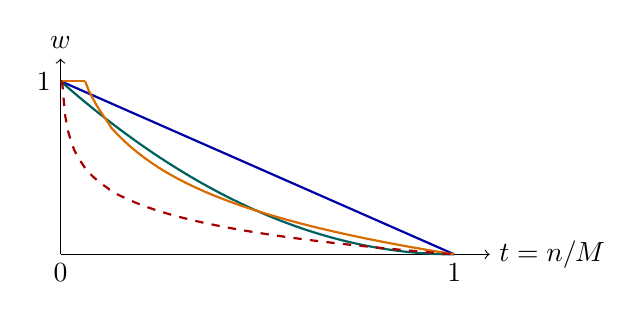
\begin{tikzpicture}[x=5cm,y=2.2cm]
\draw[->] (0,0)--(1.09,0) node[right] {\(t=n/M\)};
\draw[->] (0,0)--(0,1.13) node[above] {\(w\)};
\draw[thick,blue!65!black] (0,1)--(1,0);
\draw[thick,teal!75!black,domain=0:1,samples=60] plot (\x,{(1-\x)^2});
\draw[thick,orange!85!black] (0,1)--(.0625,1);
\draw[thick,orange!85!black,domain=.0625:1,samples=100] plot (\x,{-ln(\x)/ln(16)});
\draw[dashed,thick,red!65!black] (0,1)--(.00390625,1);
\draw[dashed,thick,red!65!black,domain=.00390625:1,samples=130] plot (\x,{-ln(\x)/ln(256)});
\node[below] at (0,0) {\(0\)};
\node[below] at (1,0) {\(1\)};
\node[left] at (0,1) {\(1\)};
\end{tikzpicture}
\par\smallskip
{\small
\textcolor{blue!65!black}{\(1-t\)}\quad
\textcolor{teal!75!black}{\((1-t)^2\)}\quad
\textcolor{orange!85!black}{logarithmic, \(M=16\)}\quad
\textcolor{red!65!black}{logarithmic, \(M=256\)}}
\caption{Fixed profiles and the changing logarithmic profile. The latter is drawn as \(\min(1,-\log t/\log M)\), which agrees with the coefficient taper on \(1/M\le t\le1\). For each fixed \(t>0\) it tends to zero as \(M\) grows.}
\label{fig:tapers}
\end{figure}

To prove this, replace the Riesz kernel by \(M^w/(w^2\log M)\). The scalar inverse transform is \((\log(M/n))_+/\log M\), by the double residue at zero. Shift the line to \(\R w=-\delta\) as in Theorem~\ref{thm:shifted}. For \(F=1/\zeta\) this gives
\[
 D_M^{\log}(s)=F(s)+\frac{F'(s)}{\log M}
       +O_{\sigma,\delta,\eta}\!\left(
          \frac{M^{-\delta}(1+|t|)^\eta}{\log M}\right)
\]
on \(\R s=\sigma\). At \(s=1\), the same calculation gives \(D_M^{\log}(1)=1/\log M+O(M^{-\delta}/\log M)\) since \(F(1)=0\) and \(F'(1)=1\). Insert these formulas in \([1-\zeta(s)(D_M^{\log}(s)-D_M^{\log}(1))]/s\). The leading transform after multiplication by \(\log M\) is \eqref{eq:logprofile}. Lemma~\ref{lem:subpower}, Cauchy's estimate for \(F'\) on a fixed substrip, and the corresponding subpower bound for \(\zeta(s)\) give square integrability. Plancherel bounds the error by \(O(M^{-\delta})\).

For \(1\le y<M\) the formula in the \(x\)-variable is exact:
\[
 (\log M)u_M^{\log}(1/y)
  =(\log M)D_M^{\log}(1)\lfloor y\rfloor-\psi(y).
\]
To verify it, expand the floors in \(g_n(1/y)\) and use \(\sum_{n\mid m}\mu(n)\log n=-\Lambda(m)\). The latter follows by taking the logarithmic derivative of the Euler product, or directly at a prime power and by cancellation over the subsets of distinct prime factors. Since the coefficient of \(\lfloor y\rfloor\) tends to one, this identifies the pointwise limit and hence the shifted \(L^2\) limit. At the critical line the proposed limiting transform has a pole at each zero on the line. The scaled estimate therefore does not extend to that norm. It gives no conclusion about unscaled convergence there.

\begin{proposition}[An interior criterion for the logarithmic taper]\label{prop:interior}
For integer \(M\ge2\), put
\[
 \widetilde u_M=u_M^{\log}
       +M\bigl(1/\log M-D_M^{\log}(1)\bigr)g_M .
\]
Then RH is equivalent to boundedness of \(\|\widetilde u_M\|_{L^2(1/M,1)}\). It is also equivalent to convergence of this norm to zero. Under RH its square is \(O(1/\log M)\).
\end{proposition}
\begin{proof}
For \(1\le y<M\), \(g_M(1/y)=\lfloor y\rfloor/M\). The last coefficient in the definition replaces \((\log M)D_M^{\log}(1)\) by one in the exact interior identity. Thus
\[
 \|\widetilde u_M\|_{L^2(1/M,1)}^2
   =\frac{1}{(\log M)^2}\int_1^M
           |\psi(y)-\lfloor y\rfloor|^2\frac{\dd y}{y^2}.
\]
Under RH, Cram\'er's mean-square estimate gives
\(\int_Y^{2Y}|\psi(y)-y|^2\dd y\ll Y^2\), as recalled in \cite{bpt}. Replacing \(y\) by \(\lfloor y\rfloor\) changes this upper bound by at most a fixed factor and \(O(Y)\). Each dyadic block therefore contributes \(O(1)\) to the weighted integral. Summing gives the asserted rate.

Conversely, bounded interior norms give a weighted integral \(O((\log(2M))^2)\). On every dyadic block \([Y,2Y]\), Cauchy--Schwarz then bounds \(\int_Y^{2Y}|\psi(y)-\lfloor y\rfloor|y^{-\sigma-1}\dd y\) by \(O_\sigma((\log(2Y))Y^{1/2-\sigma})\). Thus the Mellin transform of \(\psi(y)-\lfloor y\rfloor\) is holomorphic on \(\R s>1/2\). For \(\R s>1\) it equals \((-\zeta'(s)/\zeta(s)-\zeta(s))/s\), by the absolutely convergent Dirichlet series of \(\Lambda\) and of the constant sequence. A zero in \(\R s>1/2\) would give a pole there, and the functional equation completes the implication to RH. Convergence implies boundedness, which closes the equivalence.
\end{proof}

\subsection{The tail and quantitative tests at a zero}

Write \(\ell=\log M\), \(E(y)=\lfloor y\rfloor-\psi(y)\) and
\(q_M=M(1-\ell D_M^{\log}(1))\). The balanced residual has the exact formula
\begin{equation}\label{eq:log-all-y}
 \ell\widetilde u_M(1/y)=E(y)
 -\sum_{M<n\le y}\mu(n)\log(n/M)\lfloor y/n\rfloor
 -q_M\lfloor y/M\rfloor,\qquad y\ge1.
\end{equation}
Indeed the untruncated sum with weight \(\mu(n)\log(M/n)\lfloor y/n\rfloor\) is
\(\ell+\psi(y)\). On removing its terms with \(n>M\), expanding the balanced dilates, and inserting the coefficient of \(g_M\), one obtains \eqref{eq:log-all-y}. The tail norm squared on \(0<x<1/M\) is the integral of the squared right-hand side against \(\ell^{-2}y^{-2}\dd y\) on \(y>M\). The terms must be kept together in this expression.

For any sequence \(u_M\) in \(L^2(0,1)\) with \(\|u_M\|_\sigma\to0\) at one \(\sigma>1/2\), convergence in the critical norm holds if and only if
\[
 \lim_{r\downarrow0}\limsup_{M\to\infty}\int_0^r|u_M(x)|^2\dd x=0.
\]
The necessity follows by bounding the tail by the whole integral. For sufficiency, the part on \([r,1]\) is at most \(r^{1-2\sigma}\|u_M\|_\sigma^2\). For instance, \(u_M=\sqrt M\one_{(0,1/M)}\) has critical norm one and shifted norm squared \(M^{1-2\sigma}/(2\sigma)\). Convergence at every fixed shifted exponent thus allows concentration at the endpoint. For the explicit linear taper, splitting at \(r=M^{-a}\) and using \(\|u_M\|_\sigma\ll M^{-\delta}\) and \(|u_M|\ll M\) gives the upper bound \(O(M^{a(2\sigma-1)-2\delta}+M^{2-a})\) for the critical norm squared. These estimates require both \(a>2\) and \(a<\delta/(\sigma-1/2)\le1\) to give decay.

\begin{proposition}[Growth forced by an off-line zero]\label{prop:two-pole-bounds}
Let \(\rho\) be a zeta zero of order \(m\) with \(\beta=\R\rho>1/2\), and set \(I(Y)=\int_1^Y|E(y)|^2\dd y/y^2\). Then
\begin{align*}
 \limsup_{X\to\infty}\frac{|B(X)|}{X^\beta(\log X)^{m-1}}
 &\ge \frac{m|\Gamma(\rho)\zeta(2\rho)|}{|\zeta^{(m)}(\rho)|},\\
 \limsup_{Y\to\infty}\frac{I(Y)}{Y^{2\beta-1}}
 &\ge \frac{m^2}{(2\beta-1)|\rho|^2}.
\end{align*}
\end{proposition}
\begin{proof}
If the first limit superior is finite, denote it by \(A\). For any \(a>A\), the large-\(X\) portion of the integral in \eqref{eq:gamma} is holomorphic for \(\R s>\beta\). At \(s=\rho+\varepsilon\), multiplying it by \(\varepsilon^m\) gives a modulus bounded by \(a(m-1)!\), using
\(\int_1^\infty X^{-\varepsilon}(\log X)^{m-1}\dd X/X=(m-1)!/\varepsilon^m\).
The bounded-\(X\) portion tends to zero after multiplication. By continuation from \(\R s>1\), the limit is the leading Laurent coefficient \(m!\Gamma(\rho)\zeta(2\rho)/\zeta^{(m)}(\rho)\). Let \(a\downarrow A\).

For the second inequality put \(\alpha=2\beta-1>0\). If the second limit superior is \(C<\infty\), choose \(c>C\) so that \(I(y)\le c y^\alpha\) for all sufficiently large \(y\). For \(\varepsilon>0\), integration by parts gives
\[
 \int_1^\infty y^{-\alpha-\varepsilon}\dd I(y)
 \le O(1)+c\frac{\alpha+\varepsilon}{\varepsilon}
 \qquad (0<\varepsilon\le1).
\]
Cauchy--Schwarz applied to the Mellin transform \(F_E(s)=\int_1^\infty E(y)y^{-s-1}\dd y\) now gives
\[
 |F_E(\rho+\varepsilon)|^2
 \le \left(\int_1^\infty y^{-\alpha-\varepsilon}\dd I(y)\right)
      \left(\int_1^\infty y^{-2\beta-\varepsilon+\alpha}\dd y\right)
 =\frac1\varepsilon\int_1^\infty y^{-\alpha-\varepsilon}\dd I(y).
\]
The same bound on absolute integrals is locally uniform for \(\R s>\beta\), so the transform is holomorphic there. Its continuation from \(\R s>1\) is \((\zeta(s)+\zeta'(s)/\zeta(s))/s\), as in Proposition~\ref{prop:interior}. The residue at \(\rho\) is \(m/\rho\). Taking \(\varepsilon\downarrow0\) yields \(m^2/|\rho|^2\le c\alpha\), and then \(c\downarrow C\) proves the bound. Infinite limit superiors require no estimate.
\end{proof}

Since \(I\) is nondecreasing, the second lower bound also holds with \(Y\) restricted to integers. By Proposition~\ref{prop:interior}, it gives a positive lower limit superior for \(M^{1-2\beta}(\log M)^2\|\widetilde u_M\|_{L^2(1/M,1)}^2\). At a high zero the Gamma factor in the first inequality is small, but the exponent \(\beta\) still exceeds \(1/2\). A zero-density estimate allows isolated zeros in this range. To exclude them by either route requires an upper estimate that contradicts the corresponding lower bound.

\begin{corollary}[Power growth of the balanced logarithmic taper]
If \(\Theta\) is the supremum of the real parts of the nontrivial zeros, then
\[
 \limsup_{M\to\infty}
 \frac{\log(1+\|\widetilde u_M\|_{1/2})}{\log M}
 =\Theta-\frac12 .
\]
\end{corollary}
\begin{proof}
For \(\Theta>1/2\), Proposition~\ref{prop:two-pole-bounds} gives a lower bound \(\beta-1/2\) for each zero with \(\beta>1/2\). The added one makes the lower bound zero automatic if \(\Theta=1/2\).

For the upper bound take \(s=1/2+it\) in the Mellin integral for \(D_M^{\log}(s)\) and move the \(w\)-line from two to \(\Theta-1/2+\delta>0\), for \(0<\delta<1/4\). The rectangle has no poles. Lemma~\ref{lem:subpower} bounds the reciprocal on the new line by \(O_{\delta,\eta}((1+|t+\operatorname{Im}w|)^\eta)\) for every \(\eta>0\) if \(\Theta<1\), and absolute convergence suffices if \(\Theta=1\). As for the linear taper, the kernel's quadratic decay gives
\[
 |D_M^{\log}(1/2+it)|
 \ll_{\delta,\eta} \frac{M^{\Theta-1/2+\delta}(1+|t|)^\eta}{\log M}.
\]
The Mellin formula for \(u_M^{\log}\), convexity on the critical line, and Plancherel give \(\|u_M^{\log}\|_{1/2}\ll_\delta M^{\Theta-1/2+\delta}\), since \(D_M^{\log}(1)=O(\log M)\) and one may take \(\eta<1/8\).

The bound \(\|g_M\|_{1/2}\ll M^{-1/2}\) follows from \(|g_M|\le2\) on \((0,1/M)\) and \(|g_M(x)|\le1/(Mx)\) on \([1/M,1]\). If \(\Theta<1\), the double-residue calculation at \(s=1\) with \(w\)-line \(\Theta-1+\delta\), for \(0<\delta<1-\Theta\), gives
\[
 D_M^{\log}(1)=1/\log M+O_\delta(M^{\Theta-1+\delta}/\log M).
\]
The balancing term thus has norm \(O_\delta(M^{\Theta-1/2+\delta}/\log M)\). For \(\Theta=1\) the elementary bound for \(D_M^{\log}(1)\) instead gives \(O(\sqrt M\log M)\). Combining the bounds and sending \(\delta\downarrow0\) gives the upper exponent. In the case \(\Theta=1/2\), this exponent alone gives no critical-norm convergence.
\end{proof}

\subsection{What the quasi-Riemann proof transfers}

In Theorem 1.1 of the September 30 manuscript \cite{oai}, the zero-free statement is proved first for the finite-order Hecke family over \(\mathbb Q(\sqrt{-3})\), and then transferred to Dirichlet \(L\)-functions by quadratic factorization. The underlying continuation step compares two estimates for the same smoothed inverse signal. To describe its logic, write \(b\) for a hypothetical supremum of the real parts of the zeros in the family and \(\theta_0<b\) for the proposed threshold. Suppose a smoothed Mellin signal with a nonvanishing multiplier has a comparison \(J(X)\) satisfying
\begin{align*}
 J(X)&=O(X^{\theta_0+c+\omega}),\\
 J(X)-\operatorname{signal}(X)&=O(X^{b+c-\tau}),
 \qquad 0<\omega<b-\theta_0,\quad \tau>0 .
\end{align*}
Taking the triangle inequality gives \(O(X^{b+c-\min(b-\theta_0-\omega,\tau)})\). If the exponent saving is uniform over the family, Mellin continuation of the type in \eqref{eq:gamma}, with the shift \(c\), rules out a zero arbitrarily close to \(b\). The arithmetic work is in obtaining the two estimates with a uniform positive margin. Part I, Theorem 3.1, uses a completed cubic-theta sum and gives \(11/12\). Part II uses prime compensation, asymmetric scales and two additional moment estimates to get \(7/8\). Section 20 combines those moment estimates with the row counts.\footnote{The Mellin division step is safe only when the multiplier is nonvanishing in the region being tested. Proposition 2.1 of \cite{oai} uses a Gaussian and a holomorphic factor within \(1/2\) of one.}

The final factorization can be seen directly at each unramified prime. Let \(\chi_{-3}\) be the quadratic character of \(\mathbb Q(\sqrt{-3})/\mathbb Q\). At a split prime \(p\), the norm lift of \(\chi\) has two factors \((1-\chi(p)p^{-s})^{-1}\). At an inert prime, the factor is \((1-\chi(p)^2p^{-2s})^{-1}\), which equals the product of the factors with \(\chi(p)\) and \(-\chi(p)\). These are precisely the two Dirichlet factors of \(L(s,\chi)L(s,\chi\chi_{-3})\). Excluding the finitely many ramified and conductor primes gives the identity for incomplete products in \(\R s>1\), then by meromorphic continuation. Removed Euler factors are nonzero on \(\R s>0\). This transfers nonvanishing away from the principal pole. At \(s=1\), use the classical nonvanishing of nonprincipal Dirichlet \(L\)-functions.

The P\'olya--Vinogradov v3 paper \cite{pv} uses the \(11/12\) input in Theorem 1.5. Its Proposition 3.7 applies a Riesz kernel to prime sums in a rectangle, and its Theorem 1.1 combines this with additive dissection and harmonic weights. We use the Riesz kernel in Theorem~\ref{thm:shifted}, where the object is an inverse zeta polynomial. The character-sum bound in \cite{pv} does not transfer to the shifted Liouville products. For instance \(a(n)=\lambda(n)\lambda(n+1)\) has \(a(3)=-1\), \(a(7)=1\) and \(a(21)=1\). It fails the multiplicative identity on the coprime pair \(3,7\). Nor does the fixed \(11/12\) or \(7/8\) continuation estimate provide the needed uniform margin at \(1/2\).


\section{The character version and GRH}\label{sec:characters}

For a Dirichlet character \(\chi\), including the primitive character of conductor \(1\), put \(a_\chi(n)=\lambda(n)\chi(n)\). Define \(L_\chi^\lambda(N)=\sum_{n\le N}a_\chi(n)\) and
\[
 Q_\chi(N)=\frac1N\sum_{t\in\mathbb Z}
  \left|\sum_{t<n\le t+N}a_\chi(n)\one_{[1,N]}(n)\right|^2 .
\]
The boundary identity \eqref{eq:fejerboundary} holds with complex moduli in each term. Thus
\(\tfrac12|L_\chi^\lambda(N)|^2\le Q_\chi(N)
 \le5\max_{j\le N}|L_\chi^\lambda(j)|^2\).
The Fourier identity holds as well, with
\(C_h=\sum_{n\le N-h}a_\chi(n+h)\overline{a_\chi(n)}\)
and the real part of its weighted sum.

\begin{theorem}[Signed energy for Dirichlet characters]\label{thm:char-grh}
Let \(1/2\le\theta\le1\). The following conditions are equivalent.
\begin{enumerate}
\item Every Dirichlet \(L\)-function has no zero in \(\R s>\theta\).
\item For every fixed character \(\chi\) and every \(\varepsilon>0\),
 \(L_\chi^\lambda(N)\ll_{\chi,\varepsilon}N^{\theta+\varepsilon}\).
\item For every fixed character \(\chi\) and every \(\varepsilon>0\),
 \(Q_\chi(N)\ll_{\chi,\varepsilon}N^{2\theta+\varepsilon}\).
\end{enumerate}
At \(\theta=1/2\) these are equivalent to Dirichlet GRH.
\end{theorem}
\begin{proof}
The boundary inequalities give the equivalence of the second and third conditions. Under the second condition partial summation extends
\[
 F_\chi(s)=\sum_{n\ge1}\lambda(n)\chi(n)n^{-s}
         =\frac{L(2s,\chi^2)}{L(s,\chi)}
\]
holomorphically to \(\R s>\theta\). The numerator has an absolutely convergent nonvanishing Euler product there. This proves the first condition.

For the reverse implication fix \(\chi\). The proof of Lemma~\ref{lem:subpower} applies to \(L(s,\chi)\). For a nonprincipal character, the partial sums of \(\chi\) are bounded by its modulus, and partial summation gives \(L(s,\chi)=s\int_1^\infty(\sum_{n\le x}\chi(n))x^{-s-1}\dd x\) on \(\R s>0\). This gives the polynomial growth on the disks used in that lemma. The Euler product normalizes the logarithm at the center. For a principal character use \(\zeta(s)\) times its finitely many Euler factors. Each is nonzero on \(\R s>0\). The three-circles argument gives reciprocal subpower growth for this fixed \(\chi\), uniformly in each closed strip to the right of \(\theta\). The numerator \(L(2s,\chi^2)\) is bounded on such a strip because \(2\R s>1\). Apply the truncated Perron proof of Proposition~\ref{prop:perron}, using \(|\lambda(n)\chi(n)|\le1\). This proves the second condition. At \(\theta=1\), it is trivial and the Euler product gives the first. The functional equations for primitive characters complete the final assertion.
\end{proof}

No uniform bound on the dependence of the constants on the conductor is assumed here. To obtain GRH, the estimates must nevertheless hold for every fixed character and at all sufficiently large \(N\). The quasi-Riemann input specializes this criterion to \(\theta=7/8\), giving \(Q_\chi(N)\ll_{\chi,\varepsilon}N^{7/4+\varepsilon}\). The desired exponent is \(1+\varepsilon\).


\section{Smoothing across Dirichlet conductors}\label{sec:conductors}

For \(X>0\), define the smoothed twists and their weighted mean square by
\begin{align*}
 B_\chi(X)&=\sum_{n\ge1}\lambda(n)\chi(n)e^{-n/X},\\
 A_*(X)&=\sum_{q\ge1}\frac{1}{q^2\varphi(q)}
                 \sum_{\chi\bmod q}^{*}|B_\chi(X)|^2 .
\end{align*}
The star restricts to primitive characters. The character of conductor one is included. Absolute convergence follows from \(|B_\chi(X)|\le X\), since \(\sum_{n\ge1}e^{-n/X}=(e^{1/X}-1)^{-1}\le X\).

\begin{theorem}[Large conductors]\label{thm:large-conductors}
For \(X>0\) and \(Q\ge1\),
\[
 \sum_{q\ge Q}\frac{1}{q^2\varphi(q)}
       \sum_{\chi\bmod q}^{*}|B_\chi(X)|^2
 \ll X^2Q^{-3}+XQ^{-1}.
\]
The constant is absolute. In particular, for \(X\ge1\) the contribution from \(q\ge X^{1/3}\) is \(O(X)\). The same bound holds if one includes imprimitive characters with primitive conductor at least \(Q\) and weights each character by its modulus.
\end{theorem}
\begin{proof}
Put \(T_\chi(y)=\sum_{n\le y}\lambda(n)\chi(n)\), interpreted as zero for \(y<1\). On a block \(R\le q<2R\), use \(1/(q^2\varphi(q))\le R^{-3}q/\varphi(q)\). The multiplicative large sieve \cite{mv-large} gives
\[
 \sum_{R\le q<2R}\frac{1}{q^2\varphi(q)}
             \sum_{\chi\bmod q}^{*}|T_\chi(y)|^2
 \ll R^{-3}(y+4R^2)y .
\]
The square norm of the coefficient sequence in the sieve is at most \(y\). Partial summation writes \(B_\chi(X)=X^{-1}\int_0^\infty T_\chi(y)e^{-y/X}\dd y\). Minkowski's integral inequality in the weighted Euclidean norm bounds the square root of the block contribution by
\[
 \frac{C}{XR^{3/2}}\int_0^\infty(y+2R\sqrt y)e^{-y/X}\dd y
 \ll XR^{-3/2}+\sqrt{X/R}.
\]
Squaring and summing over \(R=2^jQ\), \(j\ge0\), gives the assertion for primitive characters. This argument applies to all sequences of modulus at most one.

For a character modulo \(rk\) induced by a primitive character \(\chi_*\) modulo \(r\), inclusion-exclusion and complete multiplicativity give
\[
 B_\chi(X)=\sum_{d\mid k}\mu(d)\lambda(d)\chi_*(d)B_{\chi_*}(X/d).
\]
The factors at primes dividing \(r\) vanish automatically. For fixed \(k\) there is one lift per primitive character, and \(\varphi(rk)\ge\varphi(r)\varphi(k)\) by the prime-power formula. Apply the triangle inequality to the weighted norm over all \(r\ge Q\) in this layer. Its upper bound is
\[
 \frac{C\tau(k)}{k\sqrt{\varphi(k)}}
       \bigl(XQ^{-3/2}+\sqrt{X/Q}\bigr),
\]
using the primitive bound at \(X/d>0\) and \(|\mu(d)\lambda(d)\chi_*(d)|\le1\). Squaring and summing over \(k\) is allowed because \(\sum_{k\ge1}\tau(k)^2/(k^2\varphi(k))<\infty\), by the elementary divisor bound.
\end{proof}

For the uniform estimate over completely multiplicative signs, the term \(X^2/Q^3\) is necessary. Choose an odd prime \(r\asymp Q\), \(r\ge Q\), and extend the Legendre character \(\chi_r\) to a sign function \(f\) by setting \(f(r)=1\) and keeping complete multiplicativity. The \(\chi_r\) twist of \(f\) is the indicator of integers coprime to \(r\), so its smoothed sum is \(\gg X\) for \(X\ge2\). That single primitive term contributes \(\gg X^2/Q^3\).

\begin{theorem}[Exact exponent across conductors]\label{thm:conductor-exponent}
Let \(\Theta_D\) be the supremum of real parts of nontrivial zeros over primitive Dirichlet \(L\)-functions, including \(\zeta\). Then
\[
 \limsup_{X\to\infty}\frac{\log(1+A_*(X))}{\log X}
 =2\Theta_D .
\]
\end{theorem}
\begin{proof}
Write \(r\) for the limit superior. Every fixed character has positive weight, so \(B_\chi(X)\ll_{\chi,\varepsilon} X^{r/2+\varepsilon}\). For \(\R s>1\), the Mellin identity is
\[
 \int_0^\infty B_\chi(X)X^{-s}\frac{\dd X}{X}
 =\Gamma(s)\frac{L(2s,\chi^2)}{L(s,\chi)} .
\]
The integral near zero is entire by exponential decay. At a zero \(\rho\) with \(\R\rho>1/2\), the numerator has a nonvanishing Euler product and Gamma has no zeros. If \(r/2<\R\rho\), take \(\varepsilon\) smaller than the difference. The growth bound then extends the integral holomorphically across \(\rho\), a contradiction. For the conductor-one character, the quotient also has a pole at \(s=1/2\) from \(\zeta(2s)\), since \(\zeta(1/2)\ne0\) by the alternating-series formula. This gives \(r\ge1\) even when \(\Theta_D=1/2\).

If \(\Theta_D=1\), the bound \(A_*(X)\ll X^2\) gives the upper estimate. Otherwise fix \(\Theta_D<\sigma<1\). For every \(\eta>0\) there is a constant independent of \(q\) and \(t\) with
\[
 |L(u+it,\chi)^{-1}|
 \ll_{\sigma,\Theta_D,\eta}(q(2+|t|))^\eta
 \qquad(\sigma\le u\le2).
\]
For a nonprincipal character the sums over complete periods vanish and the partial sums have modulus at most \(q\). Partial summation gives \(|L(s,\chi)|\le q|s|/\R s\) on \(\R s>0\). To get the reciprocal bound, use the disks of Lemma~\ref{lem:subpower} centered at \(2+it\), with radii
\(1/2<2-\sigma<R_2<R<2-\Theta_D\).
The logarithm normalized at the center by the Euler product has real part \(O(\log(q(2+|t|)))\) from above on radius \(R\). Borel--Carath\'eodory gives the same bound on its modulus on radius \(R_2\), and the Euler product bounds it absolutely on radius \(1/2\). Three circles at radius \(2-\sigma\) give a bound by a fixed power less than one of \(\log(q(2+|t|))\). Exponentiating yields the displayed estimate. For conductor one use Lemma~\ref{lem:subpower}, with the reciprocal extended by zero at the principal pole.

Inverting the exponential Mellin transform and shifting from \(\R s=2\) to \(\R s=\sigma\) gives \(|B_\chi(X)|\ll_{\sigma,\Theta_D,\eta}q^\eta X^\sigma\). The quotient is holomorphic on this strip and its numerator is bounded there by \(\zeta(2\sigma)\). Stirling's formula supplies exponential decay on the horizontal edges and integrability on the new line. Choose \(0<\eta<1/2\) and sum over conductors. Since \(\sum_q q^{-2+2\eta}<\infty\), we obtain \(A_*(X)\ll X^{2\sigma}\). Let \(\sigma\downarrow\Theta_D\).
\end{proof}

By the functional equations, Dirichlet GRH holds if and only if \(\Theta_D=1/2\). The two theorems therefore reduce this approach to
\[
 \sum_{q<X^{1/3}}\frac{1}{q^2\varphi(q)}
       \sum_{\chi\bmod q}^{*}|B_\chi(X)|^2
       \ll_\varepsilon X^{1+\varepsilon}
       \qquad(\varepsilon>0).
\]
The estimate remains open. Conductor one alone contributes \(|B_{\chi_1}(X)|^2\), so positive averaging retains the original RH obstruction.

\subsection{Orthogonality and square divisors}

Write \(A(X)\) for the sum over all characters. Orthogonality on the reduced residue classes yields
\[
 A(X)=\sum_{n,m\ge1}\lambda(n)\lambda(m)e^{-(n+m)/X}
          \sum_{\substack{q\mid n-m\\(q,n)=1}}q^{-2}.
\]
All positive \(q\) divide zero in the diagonal term. The innermost sum is bounded by \(\zeta(2)\), which justifies rearrangement. The diagonal equals
\[
 \zeta(2)\sum_{d\ge1}\frac{\mu(d)}{d^2(e^{2d/X}-1)}
 =\frac{\zeta(2)}{2\zeta(3)}X+O(1).
\]
Indeed, inclusion-exclusion gives \(\sum_{(q,n)=1}q^{-2}=\zeta(2)\sum_{d\mid n}\mu(d)d^{-2}\). Summing over multiples of \(d\) gives the geometric denominator. Use \((e^y-1)^{-1}=y^{-1}+O(1)\) uniformly for \(y>0\), and sum the absolutely convergent series. The signed off-diagonal includes \(|B_{\chi_1}(X)|^2-\sum_ne^{-2n/X}\).

The prime-power identities
\[
 \lambda(n)=\sum_{d^2\mid n}\mu(n/d^2),\qquad
 \mu(n)=\sum_{d^2\mid n}\mu(d)\lambda(n/d^2)
\]
give two vector relations. Let \(M_\chi(X)=\sum_{n\ge1}\mu(n)\chi(n)e^{-n/X}\), and let \(U_d\) act on the \(\chi\)-coordinate by multiplication by \(\chi(d)^2\). Then
\[
 B(X)=\sum_{d\ge1}U_d M(X/d^2),\qquad
 M(X)=\sum_{d\ge1}\mu(d)U_d B(X/d^2).
\]
The series are absolutely convergent in the weighted norm because the smoothed sums are bounded absolutely by \(X/d^2\). Each \(U_d\) is a contraction. A bound \(O_\varepsilon(X^{1/2+\varepsilon})\) in either weighted norm transfers to the other by Minkowski and \(\sum_d d^{-1-2\varepsilon}<\infty\). Exponential decay gives the same upper bound for \(0<X<1\) with a changed constant. Both factorizations leave the small-conductor cancellation in the \(d=1\) term.

\subsection{Why increasing the modulus retains conductor one}
\label{ssec:principal-conductor}

The large-conductor estimate is indexed by primitive conductor, which
is different from the modulus of an induced character. The distinction
is exact for the principal character $\chi_{0,p}$ modulo a prime $p$:
\begin{equation}\label{eq:principal-lifting}
 B_{\chi_{0,p}}(X)=B(X)+B(X/p).
\end{equation}
Indeed the removed multiples of $p$ contribute
$\lambda(p)B(X/p)=-B(X/p)$. Thus, if $X\ge2$ and
$p\ge2X\log X$,
\[
 |B_{\chi_{0,p}}(X)-B(X)|
 \le(e^{p/X}-1)^{-1}\le(X^2-1)^{-1}\le2X^{-2}.
\]
This large-modulus twist still has primitive conductor one, and is
excluded from the large-primitive-conductor tail in
Theorem~\ref{thm:large-conductors}. On the Mellin side the multiplier
is $1+p^{-s}$, which is nonzero for $\R s>0$ and preserves every
right-hand pole. Formula~\eqref{eq:principal-lifting} is also checked
coefficientwise in \texttt{anc/check\_primitive\_identities.py}.

There is a separate obstruction to a coefficient-uniform reverse
inequality. For a bounded sequence $a$, put
\[
 \operatorname{Tail}_a(X,Q)=
 \sum_{q\ge Q}\frac1{q^2\varphi(q)}
   \sum_{\chi\bmod q}^{*}
       \left|\sum_{n\ge1}a_ne^{-n/X}\chi(n)\right|^2.
\]
The primitive-character proof of Theorem~\ref{thm:large-conductors}
applies to every $|a_n|\le1$, and gives
$\operatorname{Tail}_a(X,X^{1/3})\ll X$.
If a uniform reconstruction inequality
\[
 \left|\sum_{n\ge1}a_ne^{-n/X}\right|^2
       \le K(X)\operatorname{Tail}_a(X,X^{1/3})
\]
were available, then necessarily $K(X)\gg X$ whenever it holds.
To see this, use the completely multiplicative sequence $a_n=1$,
whose untwisted sum is $(e^{1/X}-1)^{-1}\sim X$. Its square is of
order $X^2$, whereas the tail is $O(X)$. Thus no such uniform
reconstruction can have $K(X)=O(X^\kappa)$ with $\kappa<1$.
Even a hypothetical reconstruction with the smallest compatible
scale $K(X)\asymp X$ would give only an $O(X^2)$ upper estimate
when combined with the tail bound; a larger coefficient would
weaken it further. A stronger reconstruction for Liouville would
need additional arithmetic cancellation.



\section{A direct local-energy construction}\label{sec:local-energy}

We now attack the single smoothed sum \(B\) of
Proposition~\ref{prop:smoothed}. The construction in this section
controls point evaluation by a neighboring-scale mean square without
assuming a zero-free half-plane. It then separates a computable
diagonal from the signed arithmetic term still requiring an estimate.
The results of this section do not establish that estimate.

\subsection{Reconstruction with a logarithmic cost}

For any complex sequence with \(|a_n|\le1\), put
\[
 F(X)=\sum_{n\ge1}a_ne^{-n/X},\qquad
 \mathcal H_F(X)=\int_{X/2}^{2X}|F(Y)|^2\frac{\dd Y}{Y}.
\]
Both expressions converge absolutely for \(X>0\).

\begin{theorem}[Explicit analytic localization]\label{thm:analytic-local}
For \(X\ge1\) and \(m=\lceil8\log_2(2X)\rceil\),
\begin{equation}\label{eq:analytic-local}
 |F(X)|^2\le10(m+2)\mathcal H_F(X)+X^{-4}.
\end{equation}
There is an explicit degree-\(m\) polynomial kernel \(K_m(0,u)\)
on \([-1/4,1/4]\) such that
\[
 F(X)=\int_{-1/4}^{1/4}K_m(0,u)
             F\!\left(\frac X{1+u}\right)\dd u+\mathcal R_X,
 \qquad
 |\mathcal R_X|\le\frac{\sqrt{2(m+2)}}{128X^7}.
\]
\end{theorem}
\begin{proof}
The holomorphic function
\[
 G_X(z)=\sum_{n\ge1}a_ne^{-n(1+z)/X}
\]
is defined for \(\operatorname{Re}z>-1\). On \(|z|\le1/2\),
\[
 |G_X(z)|\le(e^{1/(2X)}-1)^{-1}\le2X.
\]
Let \(P_m\) be its Taylor polynomial at zero. Cauchy's estimate gives
\[
 \sup_{|u|\le1/4}|G_X(u)-P_m(u)|
 \le2X\sum_{j>m}(2|u|)^j
 \le2X\,2^{-m}=:\delta.
\]
In particular \(P_m(0)=G_X(0)=F(X)\) exactly.

Let \(L_j\) denote the Legendre polynomial normalized by \(L_j(1)=1\).
Its norm on \([-1,1]\) is \(2/(2j+1)\). For completeness these
identities follow from Rodrigues' formula
\[
 L_j(t)=\frac1{2^j j!}\frac{\dd^j}{\dd t^j}(t^2-1)^j.
\]
Integration by parts \(j\) times proves orthogonality to polynomials
of degree less than \(j\). Its leading coefficient is
\((2j)!/(2^j(j!)^2)\); the recurrence
\(\int_{-1}^1(1-t^2)^j\dd t
 =\frac{2j}{2j+1}\int_{-1}^1(1-t^2)^{j-1}\dd t\)
then gives the stated norm.
Thus the evaluation kernel on the shorter interval is
\[
 K_m(0,u)=2\sum_{j=0}^m(2j+1)L_j(0)L_j(4u).
\]
Expanding a polynomial in this orthogonal basis gives
\begin{equation}\label{eq:kernel-reproduce}
 P(0)=\int_{-1/4}^{1/4}K_m(0,u)P(u)\dd u,\qquad
 |P(0)|^2\le K_m(0,0)\int_{-1/4}^{1/4}|P(u)|^2\dd u.
\end{equation}
These are classical reproducing-kernel identities
\cite[\S18.2(v)]{dlmf}; their constants have been derived here.
\footnote{The polynomial approximation is applied to the analytic
function of reciprocal scale, not to the arithmetic coefficients.
It therefore does not assume cancellation of \(\lambda\).}

Rodrigues' formula also gives
\[
 L_{2r+1}(0)=0,\quad
 L_{2r}(0)=(-1)^r\binom{2r}{r}4^{-r},\quad
 \left(\binom{2r}{r}4^{-r}\right)^2\le\frac1{r+1}.
\]
The last inequality follows by induction, since
\((2r+1)^2(r+2)\le4(r+1)^3\). Consequently
\[
 K_m(0,0)
 =2\sum_{r\le m/2}(4r+1)
      \left(\binom{2r}{r}4^{-r}\right)^2
 \le4(m+2).
\]
Apply \eqref{eq:kernel-reproduce} to \(P_m\) and use
\(|P_m|^2\le2|G_X|^2+2\delta^2\):
\[
 |F(X)|^2\le8(m+2)\int_{-1/4}^{1/4}|G_X(u)|^2\dd u
             +4(m+2)\delta^2.
\]
The substitution \(Y=X/(1+u)\) bounds this integral by
\[
 \int_{4X/5}^{4X/3}|F(Y)|^2\frac X{Y^2}\dd Y
 \le\frac54\mathcal H_F(X).
\]
Also \(\delta\le(128X^7)^{-1}\) and \(m+2\le16X\) for \(X\ge1\).
Hence \(4(m+2)\delta^2\le X^{-4}\), proving
\eqref{eq:analytic-local}. Finally
\(\int|K_m(0,u)|\dd u\le\sqrt{K_m(0,0)/2}\)
applied to \(G_X-P_m\) gives the reconstruction formula and error.
\end{proof}

In particular, \(\mathcal H_B(X)\ll_\varepsilon X^{1+\varepsilon}\)
would imply the requested pointwise square-root estimate. Only the
analytic transfer has been proved; it supplies no upper bound for
\(\mathcal H_B\).

\begin{figure}[ht]
\centering
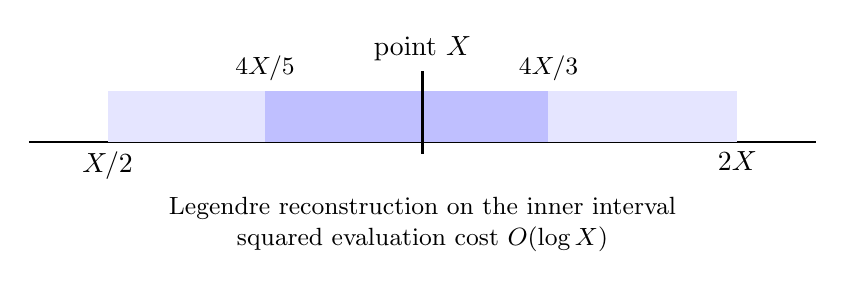
\begin{tikzpicture}[x=1cm,y=1cm]
 \draw[thick] (0,0)--(10,0);
 \fill[blue!10] (1,0) rectangle (9,.65);
 \fill[blue!25] (3,0) rectangle (6.6,.65);
 \draw[thick] (5,-.15)--(5,.9);
 \node[below] at (1,0) {\(X/2\)};
 \node[below] at (9,0) {\(2X\)};
 \node[above] at (5,.9) {point \(X\)};
 \node[above,font=\small] at (3,.65) {\(4X/5\)};
 \node[above,font=\small] at (6.6,.65) {\(4X/3\)};
 \node[align=center,font=\small] at (5,-1.05)
  {Legendre reconstruction on the inner interval\\
   squared evaluation cost \(O(\log X)\)};
\end{tikzpicture}
\caption{Localization in scale, shown schematically. The kernel
recovers the point from nearby values. Arithmetic cancellation is
still required in their mean square.}\label{fig:local-reconstruction}
\end{figure}

\subsection{The exact signed term}

Define the positive kernel
\[
 K(v)=\int_{1/2}^2e^{-v/t}\frac{\dd t}{t}
     =\int_{1/2}^2e^{-vu}\frac{\dd u}{u}.
\]
Absolute convergence gives
\begin{align}
 \mathcal H_B(X)&=\mathcal D(X)+\mathcal O(X),
       \label{eq:local-off-diagonal}\\
 \mathcal D(X)&=\int_{X/2}^{2X}
             \frac1{e^{2/Y}-1}\frac{\dd Y}{Y},\nonumber\\
 \mathcal O(X)&=2\sum_{h\ge1}\sum_{n\ge1}
    \lambda(n)\lambda(n+h)K((2n+h)/X).\nonumber
\end{align}
The symbol \(\mathcal O(X)\) in this display names a function,
not a big-\(O\) estimate.

\begin{proposition}[A diagonal with an explicit error]\label{prop:local-diagonal}
For every \(X>0\),
\[
 0<\mathcal D(X)-\left(\frac{3X}4-\log2\right)<\frac1{4X}.
\]
\end{proposition}
\begin{proof}
For \(t>0\),
\[
 0<\frac1{e^t-1}-\frac1t+\frac12<\frac t{12}.
\]
The lower inequality follows by differentiating
\((t-2)e^t+t+2\) twice. For the upper inequality, multiplication by
\(12t(e^t-1)\) reduces it to
\[
 (t^2-6t+12)(e^t-1)-12t
   =\sum_{j\ge5}\frac{(j-3)(j-4)}{j!}t^j>0.
\]
Substitute \(t=2/Y\) and integrate. The first two terms give
\(3X/4-\log2\), and the error is less than
\(\frac16\int_{X/2}^{2X}Y^{-2}\dd Y=1/(4X)\).
\end{proof}

Therefore a signed upper bound
\(\mathcal O(X)\ll_\varepsilon X^{1+\varepsilon}\)
would suffice. Replacing its terms by absolute values only gives
order \(X^2\). Positivity of \(\mathcal H_B\) gives a lower bound
for \(\mathcal O\), not the missing upper bound.

Complete multiplicativity reorganizes the same energy as
\[
 \mathcal H_B(X)=\sum_{k\ge2}c(k)
       \int_{X/2}^{2X}\frac1{e^{k/Y}-1}\frac{\dd Y}{Y},
 \qquad
 c(k)=\sum_{\substack{1\le a<k\\(a,k)=1}}
             \lambda(a)\lambda(k-a).
\]
Indeed write the two indices as \(da,db\) with \((a,b)=1\);
their signs multiply to \(\lambda(a)\lambda(b)\).
The term \(c(2)=1\) is exactly the diagonal. The remaining terms
are coprime additive correlations. The identity leaves their
cancellation to be proved.

\subsection{Why a prime Gram argument does not close the estimate}

The logarithmic identity obtained from complete multiplicativity is
\begin{align*}
 (\lambda\log)(n)&=(\lambda*(\lambda\Lambda))(n),\\
 \lambda(d)\Lambda(d)
   &=2\mathbf1_{d=\square}\Lambda(\sqrt d)-\Lambda(d).
\end{align*}
Checking prime powers proves the second line. Smoothing gives
\begin{equation}\label{eq:lambda-log-renewal}
 \sum_{n\ge1}\lambda(n)\log n\,e^{-n/X}
 =2\sum_{d\ge1}\Lambda(d)B(X/d^2)
     -\sum_{d\ge1}\Lambda(d)B(X/d).
\end{equation}
All sums converge absolutely at fixed \(X\).
However, for distinct primes \(p,q\),
\[
 \sum_{n\le N}\lambda(pn)\lambda(qn)=N.
\]
Thus prime dilations are maximally correlated in this Gram
calculation. Treating them as orthogonal would discard a full
off-diagonal. The identity \eqref{eq:lambda-log-renewal} is not a
contraction estimate.\footnote{Almost-all short-interval results
compare short and long averages \cite{mr-short}. That comparison
does not supply the square-root size of the long average required
here. We do not use a short-interval estimate with this additional
strength as an unstated premise.}

\subsection{An explicit finite-prime model}

Let \(f_y\) be completely multiplicative, equal to \(-1\) at primes
at most \(y\) and to \(+1\) at larger primes. Write
\[
 B_y(X)=\sum_{n\ge1}f_y(n)e^{-n/X},\qquad
 c_y=\prod_{p\le y}\frac{p-1}{p+1},\qquad
 G_y(\sigma)=\prod_{p\le y}
             \frac{1+p^{-\sigma}}{1-p^{-\sigma}}.
\]

\begin{theorem}[Finite-prime main term]\label{thm:finite-prime}
For \(X>0\), \(y\ge2\), and \(0<\sigma<1\),
\begin{equation}\label{eq:finite-prime}
 |B_y(X)-c_yX|\le X^\sigma G_y(\sigma).
\end{equation}
In particular, for \(y=(\log X)^2\) as \(X\to\infty\),
\[
 B_y(X)=c_yX+O(X^{1/2+o(1)}),\qquad
 B_y(X)\ge\frac{X}{2(\log X)^4}
\]
for all sufficiently large \(X\).
\end{theorem}
\begin{proof}
Define \(g_y\) multiplicatively by \(g_y(p^j)=2(-1)^j\)
for \(p\le y\), \(j\ge1\), and zero on powers of larger primes.
Prime by prime \(f_y=\mathbf1*g_y\). Hence
\[
 B_y(X)=\sum_{d\ge1}\frac{g_y(d)}{e^{d/X}-1},\quad
 \sum_{d\ge1}\frac{g_y(d)}d=c_y,\quad
 \sum_{d\ge1}\frac{|g_y(d)|}{d^\sigma}=G_y(\sigma).
\]
Only finitely many primes support \(g_y\), so these Dirichlet sums
converge absolutely for \(\sigma>0\). Also
\[
 0<\frac1t-\frac1{e^t-1}
 \le\min(1/2,1/t)\le t^{-\sigma}.
\]
Subtract \(X\sum g_y(d)/d\) and apply this term by term to obtain
\eqref{eq:finite-prime}.

The elementary Chebyshev bound gives
\(\pi(t)\ll t/\log t\), and partial summation then gives
\[
 \log G_y(1/2)\ll\sum_{p\le y}p^{-1/2}
                 \ll\frac{\sqrt y}{\log y}.
\]
The elementary details are recorded in Appendix~\ref{app:attack-checks}.
For \(y=(\log X)^2\), this is \(o(\log X)\), so
\(G_y(1/2)=X^{o(1)}\).
If \(r=\lfloor y\rfloor\), positivity of the factors gives
\[
 c_y\ge\prod_{n=2}^r\frac{n-1}{n+1}
      =\frac2{r(r+1)}\ge y^{-2}.
\]
The error \(X^{1/2+o(1)}\) is eventually less than
\(X/(2(\log X)^4)\), proving the last assertion.
\end{proof}

This is a bound for an explicitly constructed comparison function,
not for \(\lambda\). It shows that complete multiplicativity plus
agreement at all primes through \((\log X)^2\) cannot yield a
uniform square-root bound over the resulting class of functions.

\subsection{The large-prime cancellation that remains}

Put \(P^-(1)=\infty\), and define
\[
 h_y(d)=
 \begin{cases}
   2^{\omega(d)}\lambda(d),&P^-(d)>y,\\
   0,&\text{otherwise}.
 \end{cases}
\]
At a prime greater than \(y\), convolution by its local coefficients
\[
 1+2\sum_{j\ge1}(-1)^jp^{-js}
       =\frac{1-p^{-s}}{1+p^{-s}}
\]
changes the local signs of \(f_y\) to those of \(\lambda\).
Therefore \(\lambda=f_y*h_y\), and
\begin{equation}\label{eq:prime-tail-exact}
 B(X)=B_y(X)+T_y(X),\qquad
 T_y(X)=\sum_{\substack{d>1\\P^-(d)>y}}
                h_y(d)B_y(X/d).
\end{equation}
Exponential decay justifies this identity absolutely at every
fixed \(X\). With \(y=(\log X)^2\), the desired estimate would follow
from
\begin{equation}\label{eq:prime-tail-target}
 T_y(X)=-c_yX+O_\varepsilon(X^{1/2+\varepsilon}).
\end{equation}
The comparison-kernel error in Theorem~\ref{thm:finite-prime}
is already of square-root size with a subpower loss.
The signed estimate \eqref{eq:prime-tail-target} remains unproved.

% Proof-ready insertion after eq:prime-tail-target in local-energy.tex.
% Uses the classical Davenport estimate already invoked in sec:sieve.
\begin{proposition}[Prime-tail cancellation to logarithmic order]
\label{prop:prime-tail-logarithmic}
For \(y=(\log X)^2\), and every fixed \(A>0\),
\[
 T_y(X)=-c_yX+O_A\!\left(\frac{X}{(\log X)^A}\right).
\]
In particular, \(T_y(X)/(c_yX)\to-1\).
\end{proposition}
\begin{proof}
The classical uniform additive estimate of Davenport, in the
Liouville form recalled in Section~\ref{sec:sieve} and quoted in
\cite{mrt}, gives at additive frequency zero
\[
 L(t)\ll_A \frac{t}{(\log(2t))^A}
 \qquad(t\ge1).
\]
Partial summation gives the absolutely convergent identity
\[
 B(X)=\frac1X\int_1^\infty L(t)e^{-t/X}\dd t.
\]
For \(X\ge4\), the contribution from \(1\le t\le\sqrt X\)
has modulus at most \(X^{-1}\int_1^{\sqrt X}t\dd t\le1/2\).
For \(t\ge\sqrt X\), use
\(\log(2t)\ge\tfrac12\log X\) to bound the remaining part by
\[
 \frac{C_A2^A}{X(\log X)^A}
     \int_0^\infty te^{-t/X}\dd t
 =\frac{C_A2^AX}{(\log X)^A}.
\]
Consequently \(B(X)\ll_A X/(\log X)^A\).
By Theorem~\ref{thm:finite-prime} and
\eqref{eq:prime-tail-exact},
\[
 T_y(X)+c_yX
   =B(X)-\bigl(B_y(X)-c_yX\bigr)
   =O_A\!\left(\frac{X}{(\log X)^A}\right)
        +O(X^{1/2+o(1)}).
\]
For each fixed \(A\), the last error is absorbed in the first.
Finally \(c_y\ge(\log X)^{-4}\) gives
\(T_y(X)/(c_yX)=-1+O_A((\log X)^{4-A})\).
Take any \(A>4\).
\end{proof}

This proves the main-term cancellation in the actual exponential
kernel. It is a consequence of classical additive cancellation,
not a new zero-free theorem. Its error is larger than the
square-root error requested in \eqref{eq:prime-tail-target}.

\begin{proposition}[The precise power-saving endpoint]
\label{prop:prime-tail-rh-equivalence}
For \(y=(\log X)^2\), the estimate
\[
 T_y(X)+c_yX\ll_\varepsilon X^{1/2+\varepsilon}
 \quad\text{for every }\varepsilon>0
\]
is equivalent to RH.
\end{proposition}
\begin{proof}
The exact identity and Theorem~\ref{thm:finite-prime} give
\[
 T_y(X)+c_yX-B(X)=O(X^{1/2+o(1)}).
\]
Hence the asserted family of bounds holds if and only if
\(B(X)\ll_\varepsilon X^{1/2+\varepsilon}\) for every
\(\varepsilon>0\). The equivalence of the latter condition
with RH is Proposition~\ref{prop:smoothed}.
\end{proof}


There is a cancellation theorem in a different, convergent weight.
For real \(s>1\), Euler products give
\begin{equation}\label{eq:prime-tail-abel}
 H_y(s):=\sum_{d\ge1}\frac{h_y(d)}{d^s}
 =\frac{\zeta(2s)}{\zeta(s)^2c_y(s)},\qquad
 c_y(s)=\prod_{p\le y}\frac{1-p^{-s}}{1+p^{-s}}.
\end{equation}
Uniformly for \(0<\delta\le\delta_0\) and
\(\delta\log y\le1\),
\begin{equation}\label{eq:prime-tail-double-zero}
 H_y(1+\delta)
 =\frac{\zeta(2)\delta^2}{c_y}
       \left(1+O(\delta(1+\log y))\right).
\end{equation}
Indeed the pole of \(\zeta\) at one gives
\(\zeta(2+2\delta)/\zeta(1+\delta)^2
=\zeta(2)\delta^2(1+O(\delta))\), while
\[
 \frac{\dd}{\dd s}\log c_y(s)
 =2\sum_{p\le y}\frac{(\log p)p^{-s}}{1-p^{-2s}}
 \ll\log y\quad(s\ge1)
\]
by Chebyshev and partial summation. Integrating this derivative
proves the uniform factor in \eqref{eq:prime-tail-double-zero}.
For fixed \(y\), the tail without \(d=1\) tends to \(-1\).
This is an actual all-prime cancellation in the Abel weight.

The distinction between the two kernels is essential.
\footnote{The positive absolute-coefficient series is
\(\sum |h_y(d)|d^{-s}=\zeta(s)^2c_y(s)/\zeta(2s)\);
for fixed \(y\) it has a double pole at one. Thus absolute
comparison does not preserve the small signed value in
\eqref{eq:prime-tail-double-zero}.}
Equation \eqref{eq:prime-tail-double-zero} concerns
\(d^{-1-\delta}\), whereas \eqref{eq:prime-tail-exact} contains
the scale-dependent kernel \(B_y(X/d)\). No bound for their signed
discrepancy has been obtained. Treating their cancellation as
interchangeable would assume the unresolved step.

% Suitable following the existing Abel double-zero discussion.
For clarity, the double zero in \eqref{eq:prime-tail-double-zero}
does not exclude nonreal poles. For fixed \(y\), each finite
Euler factor of \(c_y(s)\) is holomorphic and nonzero on
\(\operatorname{Re}s>0\). If \(\rho\) were a zeta zero of
order \(r\) with \(\operatorname{Re}\rho>1/2\), then
\eqref{eq:prime-tail-abel} would have the leading Laurent term
\[
 H_y(s)=
 \frac{(r!)^2\zeta(2\rho)}
      {c_y(\rho)(\zeta^{(r)}(\rho))^2}
       (s-\rho)^{-2r}
       +O((s-\rho)^{1-2r}).
\]
The coefficient is nonzero. The local cancellation at one
therefore supplies no contradiction to such a zero; excluding
it requires the global power-saving estimate.


\appendix
\section{From a fixed zero-free half-plane to summatory cancellation}\label{sec:perron}

We give the reverse implication used in Theorem~\ref{thm:equiv}. Suppose \(1/2\le\theta<1\) and \(\zeta\) has no zeros in \(\R s>\theta\). We use the classical Euler product, the meromorphic continuation and the standard truncated Perron formula as in \cite{titchmarsh}.

\begin{lemma}[Subpower growth of the reciprocal]\label{lem:subpower}
For \(0<\delta<1/4\) and \(\eta>0\),
\[
 \left|\frac{1}{\zeta(\sigma+it)}\right|
 \ll_{\theta,\delta,\eta}(1+|t|)^\eta
 \qquad(\theta+\delta\le\sigma\le2),
\]
where \(1/\zeta\) is extended by zero at \(s=1\).
\end{lemma}
\begin{proof}
Take \(|t|\ge4\) and use the disk centered at \(2+it\) of radius \(R=2-\theta-\delta/4\). The disk lies in the zero-free half-plane and misses the pole. Choose a holomorphic branch \(G=\log\zeta\) there, normalized at the center by the absolutely convergent Euler product. On the subdisk of radius \(r_0=1/2\), that product bounds \(|G|\) uniformly.

For \(\R s>0\), away from the pole, the identity
\[
 \zeta(s)=\frac{s}{s-1}-s\int_1^\infty \{x\}x^{-s-1}\dd x
\]
follows from partial summation for \(\R s>1\) and then continuation. It gives a polynomial bound on \(|\zeta|\) on the closed disk of radius \(R\), since its real parts are at least \(\theta+\delta/4\). Thus \(\max\R G\ll\log(2+|t|)\) there. Borel--Carath\'eodory with \(r_2=2-\theta-\delta/2<R\) gives \(\max_{|s-(2+it)|\le r_2}|G(s)|\ll_{\theta,\delta}\log(2+|t|)\). The branch is holomorphic on a neighborhood of that disk because the entire closed disk of radius \(R\) stays away from zeros and the pole.

The three-circles theorem at \(r_1=2-\theta-\delta\), between \(r_0\) and \(r_2\), bounds \(|G|\) by \(C(\log(2+|t|))^\tau\) for some fixed \(\tau<1\) on the disk of radius \(r_1\). This covers all points \(\sigma+it\) in the stated range. Exponentiating \(-\R G\) gives a bound by \((1+|t|)^\eta\) up to a constant. For bounded \(t\), use compactness and the removable extension of the reciprocal at the pole.
\end{proof}

\begin{proposition}[Perron calculation]\label{prop:perron}
Under the zero-free hypothesis of Lemma~\ref{lem:subpower}, \(L(x)\ll_{\theta,\varepsilon}x^{\theta+\varepsilon}\) for every \(\varepsilon>0\).
\end{proposition}
\begin{proof}
Take \(x\ge3\) a half-integer, \(c=1+1/\log x\), \(T=x^2\), and \(\sigma_0=\theta+\delta\) with \(0<\delta<\min(1/4,1-\theta,\varepsilon/2)\). Write \(F(s)=\zeta(2s)/\zeta(s)\). In the strip \(\sigma_0\le\R s\le c\), \(F\) is holomorphic and satisfies \(F(\sigma+it)\ll_{\theta,\delta,\eta}(1+|t|)^\eta\), since \(\zeta(2s)\) is bounded there by an absolutely convergent series and Lemma~\ref{lem:subpower} bounds the reciprocal. The singularity at \(s=1\) in the denominator gives a removable zero in \(F\).

Truncated Perron gives
\[
 L(x)=\frac{1}{2\pi i}\int_{c-iT}^{c+iT}F(s)\frac{x^s}{s}\dd s
 +O\!\left(\sum_{n\ge1}(x/n)^c
       \min\{1,(T|\log(x/n)|)^{-1}\}\right).
\]
Here \(|\lambda(n)|=1\). On \(x/2<n<2x\), use \(|\log(x/n)|\gg |x-n|/x\), and sum the reciprocal distances from the half-integer \(x\). Outside that range, use \(|\log(x/n)|\ge\log2\) and \(\zeta(c)\ll\log x\). The error is \(O(x\log x/T)\). Move the integral to \(\sigma_0\) in the rectangle of height \(T\). The two horizontal sides are \(O_{\theta,\delta,\eta}(x^c T^{\eta-1})\). The new vertical side is \(O_{\theta,\delta,\eta}(x^{\sigma_0}(1+T^\eta))\), by integrating \((1+|t|)^{\eta-1}\). Choose \(\eta>0\) with \(2\eta<\min(\varepsilon-\delta,1/2)\). All terms satisfy the required estimate. Every integer prefix is attained at a half-integer \(x\), and extending the bound to all real \(x\ge1\) changes only the constant.
\end{proof}

\section{The ordinary-dilate model has a different limit}\label{sec:ordinary}

For clarity about the basis in \cite{nbdraft}, define
\[
 d^{\mathrm{ord}}_M=\inf_c\Big\|1-\sum_{k\le M}c_k\{kx\}\Big\|_{L^2(0,1)}.
\]
This is the ordinary integer-dilate problem. The exact formula below is independent of the location of zeta zeros.

\begin{proposition}
Let \(J_2(d)=d^2\prod_{p\mid d}(1-p^{-2})\) and \(\varphi\) denote Euler's totient. Then
\[
 (d_M^{\mathrm{ord}})^2=\frac{1}{1+3S_M},
 \quad S_M=\sum_{d\le M}\frac{\varphi(d)^2}{J_2(d)},\qquad
 S_M\sim M\prod_p\left(1-\frac{2}{p(p+1)}\right).
\]
\end{proposition}
\begin{proof}
The centered fractional part has nonzero Fourier coefficients \(-1/(2\pi i \ell)\) at \(\ell\in\mathbb Z\setminus\{0\}\). Parseval therefore gives
\[
 \int_0^1\{jx\}\{kx\}\dd x=\frac14+\frac{\gcd(j,k)^2}{12jk}.
\]
Indeed, after writing \(j=dj_0,k=dk_0\) with \((j_0,k_0)=1\), the matching nonzero frequencies are \(j k_0 r=k j_0 r\). The corresponding coefficient products sum to \((j_0k_0)^{-1}\sum_{r\ne0}(4\pi^2r^2)^{-1}=1/(12j_0k_0)\). The constant Fourier coefficient contributes \(1/4\).

Put \(u_d=\sum_{d\mid k\le M}c_k/k\) and \(t=\sum_{k\le M}c_k\). The map from the \(c_k\) to the \(u_d\) is invertible by descending triangular elimination. The divisor identities \(\sum_{d\mid k}\varphi(d)=k\) and \(\sum_{d\mid k}J_2(d)=k^2\) follow by multiplicativity and a telescoping sum at each prime power. Thus \(t=\sum_d\varphi(d)u_d\), and the squared residual is
\[
 |1-t/2|^2+\frac{1}{12}\sum_{d\le M}J_2(d)|u_d|^2.
\]
For fixed \(t\), weighted Cauchy--Schwarz minimizes the last sum to \(|t|^2/S_M\) before the factor \(1/12\), attained by \(u_d=t\varphi(d)/(S_MJ_2(d))\). The remaining quadratic in \(t\) is minimized at \(t=6S_M/(1+3S_M)\) and has the displayed value.

Finally \(a(d)=\varphi(d)^2/J_2(d)\) is multiplicative with \(a(p^k)=(p-1)/(p+1)\) for \(k\ge1\). Thus \(a=1*b\), where \(b\) is supported on squarefree integers, \(b(p)=-2/(p+1)\), and \(b(1)=1\). Since \(\sum|b(d)|/d=\prod_p(1+2/[p(p+1)])<\infty\), dividing \(\sum_{d\le M}b(d)\lfloor M/d\rfloor\) by \(M\) and using dominated convergence gives the stated product. Every factor is positive and their deviations from \(1\) are summable.
\end{proof}

The actual Mellin transform of \(\{kx\}\) on \((0,1)\) is
\[
 \int_0^1 \{kx\}x^{s-1}\dd x
 =\frac{k}{s+1}-\frac{k-1}{s}+\frac{k^{-s}}s\sum_{r=1}^{k-1}r^s
 \quad(\R s>0).
\]
This follows by writing \(\lfloor kx\rfloor=\sum_{r=1}^{k-1}\one_{[r/k,1]}(x)\) almost everywhere and integrating. The transform cannot be replaced by a multiple of \(k^{-s}\zeta(s)/s\). For example, at \(k=1\) it is \(1/(s+1)\). Thus the \(M^{-1/2}\) distance scale proved above is about the ordinary dilates. The balanced reciprocal functions have the different Mellin image of Lemma~\ref{lem:nbmellin}.


\section{Mellin positivity and one-sided pole detection}
\label{app:mellin-positivity}

The real pole at \(s=1/2\) gives a negative bias in the smoothed
Liouville sum. It is natural to test whether one can prove an eventual
sign and thereby exclude right-hand zeros. This appendix proves
the relevant implications, including the positivity principle,
without assuming RH. An eventual sign is not proved here.

\begin{lemma}[The positivity principle]\label{lem:landau-positive}
Let \(f:[0,\infty)\to[0,\infty)\) be locally integrable, and suppose
its Laplace integral
\[
 \mathcal L(s)=\int_0^\infty f(t)e^{-st}\dd t
\]
converges for all sufficiently large real \(s\). If its abscissa
of convergence \(a\) is finite, then \(\mathcal L\) cannot extend
holomorphically to a neighborhood of the real point \(a\).
\end{lemma}
\begin{proof}
Suppose there is such a continuation, holomorphic in
\(\operatorname{Re}s>a\) and in a disc of radius \(r\) about \(a\).
Choose \(b=a+r/4\). The disc about \(b\) of radius \(r/2\)
lies in the union of those two domains. Differentiation in the
convergent integral gives the Taylor coefficients of
\(\mathcal L(b-z)\):
\[
 \frac1{j!}\int_0^\infty t^j f(t)e^{-bt}\dd t\ge0.
\]
The differentiations are justified by convergence at a real
point strictly between \(a\) and \(b\). For a real
\(z\in(r/4,r/2)\), the Taylor series converges. By Tonelli its
sum is
\[
 \int_0^\infty f(t)e^{-bt}
                 \sum_{j\ge0}\frac{(zt)^j}{j!}\dd t
 =\int_0^\infty f(t)e^{-(b-z)t}\dd t.
\]
But \(b-z<a\), contradicting the definition of the abscissa.
\end{proof}

The same principle applies to a nonnegative function \(A(X)\) on
\([X_0,\infty)\) with Mellin integral
\(\int_{X_0}^\infty A(X)X^{-s}\dd X/X\), by putting
\(X=X_0e^t\). Changing \(X_0\) only changes the meromorphic
continuation by an entire function.

\begin{theorem}[Both signs forced by a right-hand zero]
\label{thm:two-sided-smoothed}
Let \(\rho=\beta+i\gamma\) be a nontrivial zeta zero of order \(r\)
with \(\beta>1/2\). Define
\[
 C_\rho=\frac{r|\Gamma(\rho)\zeta(2\rho)|}
                     {|\zeta^{(r)}(\rho)|}>0.
\]
Then
\begin{align*}
 \limsup_{X\to\infty}
  \frac{B(X)}{X^\beta(\log X)^{r-1}}&\ge C_\rho,\\
 \liminf_{X\to\infty}
  \frac{B(X)}{X^\beta(\log X)^{r-1}}&\le-C_\rho.
\end{align*}
\end{theorem}
\begin{proof}
Put \(\Phi(s)=\Gamma(s)\zeta(2s)/\zeta(s)\).
It is the Mellin transform in \eqref{eq:gamma} for
\(\operatorname{Re}s>1\). It has no singularity at any real
point greater than \(1/2\). For \(1/2<s<1\), this follows from
\(\zeta(s)=\eta(s)/(1-2^{1-s})<0\), where the alternating
series \(\eta(s)>0\); at one the pole of \(\zeta\) gives a
removable zero in the quotient. At \(\rho\) the leading
Laurent coefficient is
\[
 A_\rho=\frac{r!\Gamma(\rho)\zeta(2\rho)}
                     {\zeta^{(r)}(\rho)}.
\]
The numerator is nonzero since \(\operatorname{Re}(2\rho)>1\).

Suppose the first inequality fails. Choose
\(0<c<C_\rho\) such that
\[
 A(X)=cX^\beta(\log X)^{r-1}-B(X)\ge0
\]
for every \(X\ge X_0\), with \(X_0>1\). Its Mellin transform
converges for real \(s>1\) and continues meromorphically as
\[
 \frac{c(r-1)!}{(s-\beta)^r}-\Phi(s)+E(s),
\]
where \(E\) is entire, accounting for the finite initial interval.
The real pole at \(\beta\) forces the abscissa of the positive
integral to be at least \(\beta\). If that abscissa were greater
than \(\beta\), the displayed continuation would be holomorphic
there, contradicting Lemma~\ref{lem:landau-positive}. Hence it
is exactly \(\beta\).

Positivity now gives, for \(\delta>0\),
\[
 \left|\int_{X_0}^\infty A(X)X^{-\beta-\delta-i\gamma}
                       \frac{\dd X}{X}\right|
 \le\int_{X_0}^\infty A(X)X^{-\beta-\delta}
                       \frac{\dd X}{X}.
\]
Multiply by \(\delta^r\) and let \(\delta\downarrow0\).
The complex pole on the left gives \(|A_\rho|\); the real
pole on the right gives \(c(r-1)!\). Therefore
\(c\ge |A_\rho|/(r-1)!=C_\rho\), a contradiction.
For the second inequality apply the identical argument to
\(A(X)=cX^\beta(\log X)^{r-1}+B(X)\).
\end{proof}

This strengthens the absolute-value pole test of
Proposition~\ref{prop:two-pole-bounds} to both one-sided
oscillations. It still gives lower bounds, not the square-root
upper bound needed to exclude \(\rho\).

\begin{proposition}[The real pole and an eventual sign]
\label{prop:eventual-smoothed-sign}
Put
\[
 c_0=-\frac{\sqrt\pi}{2\zeta(1/2)}>0.
\]
Unconditionally,
\[
 \liminf_{X\to\infty}\frac{B(X)}{\sqrt X}\le-c_0.
\]
If in addition \(B(X)\le0\) for all sufficiently large \(X\),
then RH holds, every nontrivial zero is simple, and each such
zero satisfies
\[
 \left|\frac{\Gamma(\rho)\zeta(2\rho)}{\zeta'(\rho)}\right|
 \le c_0.
\]
\end{proposition}
\begin{proof}
The function \(\Phi\) has a simple real pole at \(1/2\)
with residue \(-c_0\). Suppose the asserted limit inferior
were greater than \(-c_0\). Choose \(0<c<c_0\) such that
\(B(X)+c\sqrt X\ge0\) eventually. The Mellin transform of
this nonnegative function has continuation
\[
 \Phi(s)+\frac c{s-1/2}+E(s).
\]
Its pole at \(1/2\) has negative residue \(c-c_0\).
The positivity principle and absence of real singularities to
the right force its abscissa to be \(1/2\). The integral is
nonnegative on the real axis there, but the continuation
tends to \(-\infty\) as \(s\downarrow1/2\), a contradiction.

Now assume \(B\le0\) eventually, and apply the positivity
principle to \(-B\). Its Mellin continuation is
\(-\Phi+E\), with positive residue \(c_0\) at \(1/2\).
Its abscissa is exactly \(1/2\), by the same real-axis
argument. Thus \(\Phi\) is holomorphic in
\(\operatorname{Re}s>1/2\), which excludes all right-hand
zeros. The functional equation gives RH.

At a critical zero of order \(r\), the numerator of \(\Phi\)
is nonzero by nonvanishing of \(\zeta\) on the line
\(\operatorname{Re}s=1\). Positivity bounds the complex
Mellin integral at \(s=\rho+\delta\) by its real value at
\(s=1/2+\delta\), the latter being \(c_0/\delta+O(1)\).
The complex pole has order \(r\), so \(r\le1\), and comparison
of residues gives the displayed inequality.
\end{proof}

An eventual-sign argument would therefore need more than the
square-root estimate with an arbitrary \(X^\varepsilon\) loss:
it would also establish simplicity. Neither the sign assertion
nor the required upper bound for \(B\) has been proved.
The negative-bias lower bound alone does not control positive
excursions or rule out right-hand zeros.

\begin{proposition}[The real-pole normalization of local energy]
\label{prop:local-energy-lower}
With \(c_0\) as above, unconditionally
\[
 \limsup_{X\to\infty}\frac{\mathcal H_B(X)}X
 \ge\frac32c_0^2=\frac{3\pi}{8\zeta(1/2)^2}.
\]
\end{proposition}
\begin{proof}
There is nothing to prove if the limit superior is infinite.
Otherwise choose \(C\) greater than it, so that
\(\mathcal H_B(X)\le CX\) for all sufficiently large \(X\).
For \(\eta>0\), Tonelli and the substitution \(Y=tX\) give
\[
 \int_0^\infty\mathcal H_B(X)X^{-1-\eta}\frac{\dd X}{X}
 =r(1+\eta)P(\eta),
\]
where
\[
 r(s)=\int_{1/2}^2t^s\frac{\dd t}{t}
     =\frac{2^s-2^{-s}}s,\qquad
 P(\eta)=\int_0^\infty|B(Y)|^2Y^{-1-\eta}\frac{\dd Y}{Y}.
\]
The small-\(X\) part is uniformly finite near \(\eta=0\),
by exponential decay. The assumed large-\(X\) upper bound gives
\[
 P(\eta)\le\frac{C/\eta+O(1)}{r(1+\eta)}.
\]
For \(\delta>0\), Cauchy--Schwarz on \([1,\infty)\) now gives
\[
 \left|\int_1^\infty B(Y)Y^{-1/2-\delta}
                       \frac{\dd Y}{Y}\right|^2
 \le\frac{P(\delta)}{\delta}.
\]
The absolute integral is convergent by the same estimate.
It agrees with \(\Phi(1/2+\delta)\) up to the entire
small-\(Y\) term, by continuation from
\(\operatorname{Re}s>1\). Multiplying by \(\delta^2\) and
letting \(\delta\downarrow0\) gives
\(c_0^2\le C/r(1)=2C/3\).
Let \(C\) decrease to the limit superior.
\end{proof}

For the comparison function \(B_0(X)=-c_0\sqrt X\), the local energy
is exactly \((3/2)c_0^2X\). Thus the constant in this pole comparison
is the one dictated by the real residue. This proposition supplies
a lower constraint on any proposed upper estimate; it does not
establish such an estimate for the actual sum.

\section{Elementary prime bounds and exact checks}
\label{app:attack-checks}

Here are details of the prime estimate used in
Theorem~\ref{thm:finite-prime}. If
\(\vartheta(t)=\sum_{p\le t}\log p\), then
\(\prod_{n<p\le2n}p\) divides \(\binom{2n}{n}\le4^n\).
Summing over dyadic intervals gives
\(\vartheta(t)\le4(\log2)t\) for \(t\ge2\). Separating
primes at \(\sqrt t\) gives
\[
 \pi(t)\le\sqrt t+\frac{2\vartheta(t)}{\log t}
        \le7\,\frac t{\log t}.
\]
The last inequality uses \(\log t\le\sqrt t\).
Partial summation gives
\[
 \sum_{p\le y}p^{-1/2}
 =\frac{\pi(y)}{\sqrt y}
  +\frac12\int_2^y\frac{\pi(t)}{t^{3/2}}\dd t
 \ll\frac{\sqrt y}{\log y}.
\]
For instance split the integral at \(\sqrt y\); the first
part is \(O(y^{1/4})\) and on the second part
\(\log t\ge\frac12\log y\). This proves the asserted order
without the prime number theorem or any zero-free input.
Similarly
\(\sum_{p\le y}(\log p)/p\ll\log y\), by partial summation
of \(\vartheta\), proving the derivative bound used in
\eqref{eq:prime-tail-double-zero}.

The new checker \path{checks/attack_exact.py} uses rational
arithmetic for the following independent finite tests:
the Legendre reproducing kernel on polynomial monomials,
its evaluation norm bound, the positive coefficients of the
diagonal error, both finite-prime convolution identities,
the coprime-pair decomposition, and the prime-dilation Gram
identity. It also checks an exponential interval certificate
for \(B(1)>0\) and \(B(3)<-1/20\).
The latter rules out assigning one sign to every scale
product in \eqref{eq:lambda-log-renewal}; it is not a test
of an eventual sign.

The checker proves none of the infinite arithmetic estimates.
The analytic arguments are supplied in the text and have
not been formalized in Lean. The original finite Gram
formalization retains exactly the scope stated in the
reproduction appendix. No new RH proof, zero-free
half-plane or novelty priority is asserted in this revision.


\section{Finite Abel cancellations do not control the exponential sum}
\label{app:abel-obstruction}

Equation~\eqref{eq:prime-tail-double-zero} proves a double zero in
an Abel weight at \(s=1\). It does not prove the signed
exponential-kernel estimate \eqref{eq:prime-tail-target}. We test
the proposed implication in the larger class of bounded real
coefficients. The test below is explicit and uses neither RH
nor a hypothetical zero of the Riemann zeta function.

\begin{theorem}[A prescribed finite set of vanishing moments]
\label{thm:abel-obstruction}
Let \(k\ge1\) be an integer, \(1/2<\beta<1\), and \(\gamma>0\).
There is a real sequence \((a_n)\), with \(|a_n|\le1\), such that:
\begin{enumerate}
\item Its Dirichlet series \(D_a(s)=\sum_{n\ge1}a_nn^{-s}\)
  is absolutely convergent on \(\operatorname{Re}s>\beta\), and
  \[
   D_a^{(j)}(1)=
      \sum_{n\ge1}\frac{a_n(-\log n)^j}{n}=0
        \qquad(0\le j<k).
  \]
\item It has a meromorphic continuation with simple poles at
  \(\beta+i\gamma\) and \(\beta-i\gamma\). The Mellin transform
  \(\Gamma(s)D_a(s)\) still has those poles and has a zero of
  order at least \(k\) at \(s=1\).
\item Its exponentially smoothed sum satisfies
  \[
   S_a(X):=\sum_{n\ge1}a_ne^{-n/X}
    =\varepsilon\,\operatorname{Re}
        \bigl(\Gamma(\beta+i\gamma)X^{\beta+i\gamma}\bigr)
       +O_{k,\beta,\gamma}(1)
  \]
  for some explicitly specified \(\varepsilon>0\).
  Consequently
  \[
   \limsup_{X\to\infty}\frac{S_a(X)}{X^\beta}
       =\varepsilon|\Gamma(\beta+i\gamma)|,\qquad
   \liminf_{X\to\infty}\frac{S_a(X)}{X^\beta}
       =-\varepsilon|\Gamma(\beta+i\gamma)|.
  \]
\end{enumerate}
In particular, these \(k\) exact moment cancellations do not imply
\(S_a(X)=O(X^{1/2+\eta})\) when \(0<\eta<\beta-1/2\).
\end{theorem}

\begin{proof}
Put \(z=\beta+i\gamma\) and
\(r_n=n^{\beta-1}\cos(\gamma\log n)\). Initially retain this
coefficient except on the finite set
\[
 \mathcal S=\{2^m:0\le m<k\}.
\]
For \(0\le j<k\) define the absolutely convergent real moments
\[
 t_j=\sum_{n\notin\mathcal S}
              \frac{r_n(-\log n)^j}{n}.
\]
Convergence follows from
\(|r_n|(\log n)^j/n\le n^{\beta-2}(\log n)^j\).
We choose real numbers \(b_m\) at the indices \(2^m\) by
\begin{equation}\label{eq:moment-system}
 \sum_{m=0}^{k-1}\frac{b_m(-m\log2)^j}{2^m}
       =-t_j\qquad(0\le j<k).
\end{equation}
The matrix is invertible: after nonzero row and column
scalings it is the Vandermonde matrix \((m^j)_{j,m=0}^{k-1}\).
Its determinant is
\(\prod_{0\le m<n<k}(n-m)\ne0\).

There is also a direct finite formula for the solution. Set
\[
 \ell_m(x)=\prod_{\substack{0\le n<k\\n\ne m}}
                    \frac{x-n}{m-n}
           =\sum_{j=0}^{k-1}\ell_{m,j}x^j,\qquad
 s_j=-\frac{t_j}{(-\log2)^j}.
\]
Then
\[
 b_m=2^m\sum_{j=0}^{k-1}\ell_{m,j}s_j.
\]
Indeed, applying the moment functional
\(x^j\mapsto s_j\) to \(\ell_m\) inverts the moment system.
All the numbers \(\ell_{m,j}\) are rational.

Choose
\[
 \varepsilon=\frac1{1+\max_{0\le m<k}|b_m|}>0,\qquad
 a_n=\begin{cases}
       \varepsilon b_m,&n=2^m\in\mathcal S,\\
       \varepsilon r_n,&n\notin\mathcal S.
      \end{cases}
\]
Since \(|r_n|\le1\), all coefficients have modulus at most
one. The moment equations prove the first assertion, including
termwise differentiation at one.

For complex \(s\), absolute convergence initially gives the
holomorphic identity
\begin{equation}\label{eq:model-dirichlet}
 D_a(s)=\frac{\varepsilon}{2}
    \left(\zeta(s+1-\beta-i\gamma)
          +\zeta(s+1-\beta+i\gamma)\right)
       +\varepsilon\sum_{m=0}^{k-1}
          (b_m-r_{2^m})2^{-ms}.
\end{equation}
The finite sum is entire. The two shifted zeta functions
have distinct simple poles at the asserted points, each
with residue \(\varepsilon/2\). They are regular at one.
The moment equations give a zero there of order at least
\(k\). Multiplication by \(\Gamma(s)\), which is nonzero
and holomorphic at these points, preserves both assertions.
\footnote{For complex \(s\), the average of the two shifted
zeta functions in \eqref{eq:model-dirichlet} must be used.
Writing its real part instead would destroy holomorphy.
The displayed poles are constructed poles, not assertions
that \(\zeta(\beta\pm i\gamma)=0\).}

It remains to justify the smoothed asymptotic without any
unproved contour shift. For \(X\ge1\), apply elementary
sum--integral comparison to
\(f_X(t)=t^{z-1}e^{-t/X}\) on \([1,\infty)\). The integral
of its absolute derivative is at most
\[
 |z-1|\int_1^\infty t^{\beta-2}\dd t
   +X^{-1}\int_1^\infty t^{\beta-1}e^{-t/X}\dd t
 \le\frac{|z-1|}{1-\beta}+\Gamma(\beta).
\]
The omitted integral on \((0,1)\) has modulus at most
\(1/\beta\). Comparing on each interval \([n,n+1]\)
therefore gives the uniform estimate
\[
 \sum_{n\ge1}n^{z-1}e^{-n/X}
       =\int_0^\infty t^{z-1}e^{-t/X}\dd t+O_{\beta,\gamma}(1)
       =\Gamma(z)X^z+O_{\beta,\gamma}(1).
\]
The last identity is Euler's convergent gamma integral
\cite[\S5.9(i)]{dlmf-gamma}, here applied with
\(\operatorname{Re}z>0\). The finite coefficient changes
add only \(O_{k,\beta,\gamma}(1)\). Taking real parts
proves the asymptotic.

Finally choose
\(\log X_j=(2\pi j-\arg\Gamma(z))/\gamma\)
and the analogous sequence with an added \(\pi/\gamma\).
The two limiting normalized values have opposite signs and
the stated modulus. The uniform asymptotic bounds the
absolute normalized value by that same modulus, proving
the exact limit superior and inferior.
\end{proof}

\begin{figure}[ht]
\centering
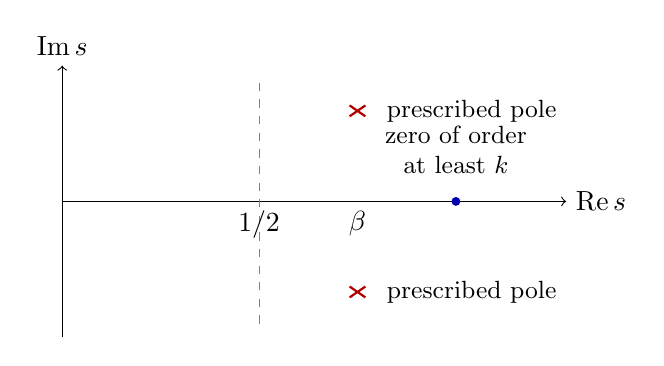
\begin{tikzpicture}[x=5cm,y=1.15cm]
 \draw[->] (0,0)--(1.28,0) node[right] {\(\operatorname{Re}s\)};
 \draw[->] (0,-1.5)--(0,1.5) node[above] {\(\operatorname{Im}s\)};
 \draw[dashed,gray] (.5,-1.35)--(.5,1.35);
 \node[below] at (.5,0) {\(1/2\)};
 \node[below] at (.75,0) {\(\beta\)};
 \fill[blue!70!black] (1,0) circle(1.6pt);
 \node[above,align=center,font=\small] at (1,.2)
     {zero of order\\at least \(k\)};
 \draw[red!70!black,thick] (.73,.94)--(.77,1.06)
                            (.73,1.06)--(.77,.94);
 \draw[red!70!black,thick] (.73,-.94)--(.77,-1.06)
                            (.73,-1.06)--(.77,-.94);
 \node[right,font=\small] at (.8,1) {prescribed pole};
 \node[right,font=\small] at (.8,-1) {prescribed pole};
\end{tikzpicture}
\caption{A model Dirichlet series in Theorem~\ref{thm:abel-obstruction}.
Any fixed number of vanishing moments at one can coexist with
the two prescribed poles. These are not claimed zeros of
the Riemann zeta function.}\label{fig:model-mellin-poles}
\end{figure}

The construction can also start with
\(r_n=n^{\beta-1}\cos(\gamma\log n-\arg\Gamma(\beta+i\gamma))\).
After the same finite adjustment its phase-aligned leading
term is \(\varepsilon|\Gamma(\beta+i\gamma)|X^\beta
\cos(\gamma\log X)\). Figure~\ref{fig:model-growth} plots
that leading term after normalization, for
\(\beta=3/4\) and \(\gamma=1\).

\begin{figure}[ht]
\centering
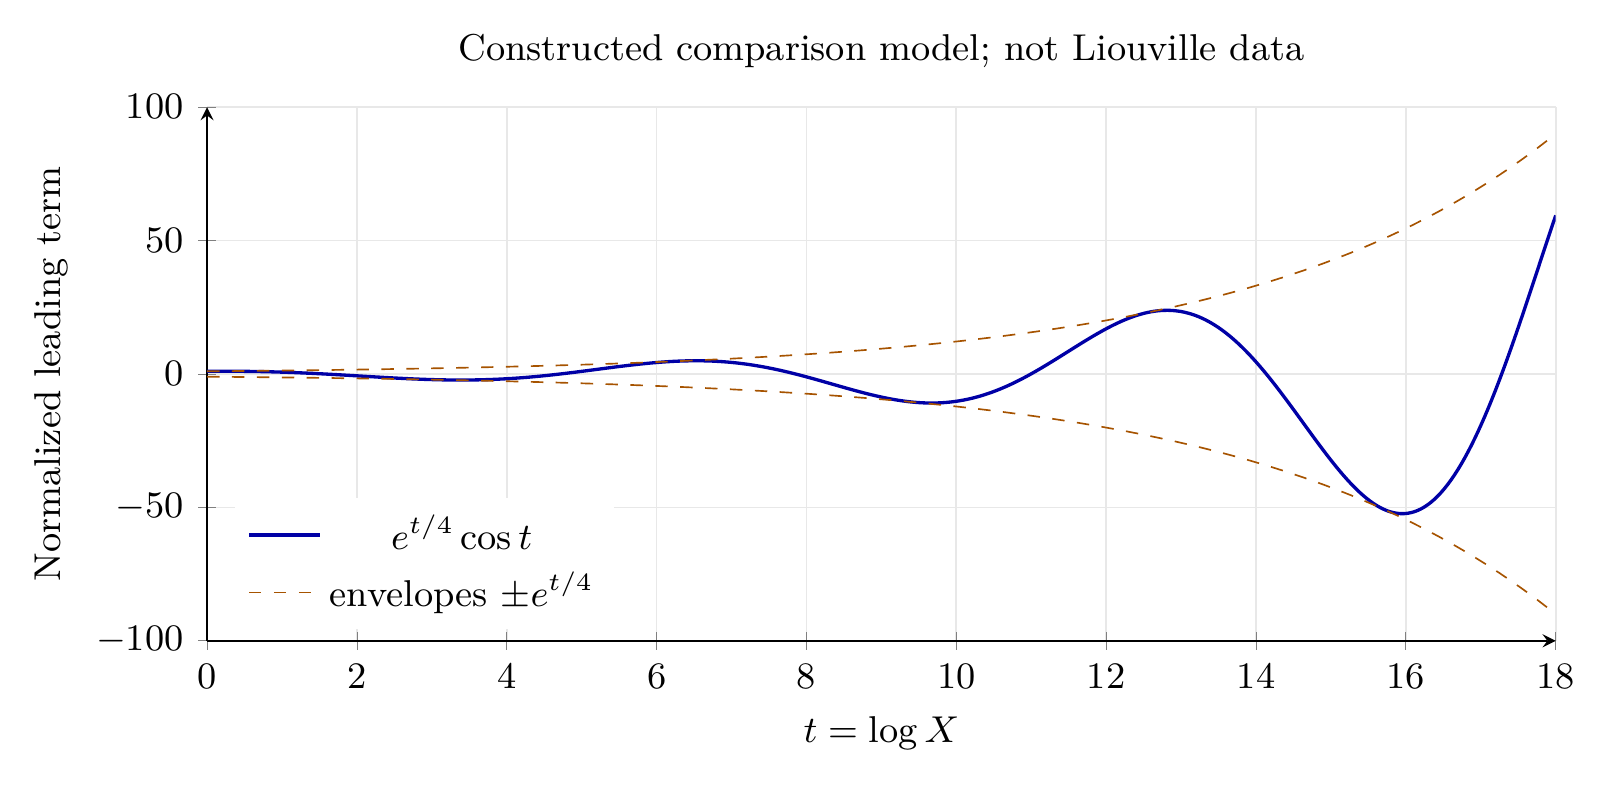
\includegraphics[width=\textwidth]{figures/model-abel-gap.png}
\caption{The phase-aligned model leading term, divided by
\(\varepsilon|\Gamma(3/4+i)|\sqrt X\), is
\(e^{t/4}\cos t\), where \(t=\log X\).
The dashed curves are its envelopes.
This is an analytic comparison model, not Liouville data or
a numerical test of RH.}\label{fig:model-growth}
\end{figure}

Theorem~\ref{thm:abel-obstruction} does not rule out a proof
that uses the full arithmetic structure of \(\lambda\).
Its coefficients are not required to be multiplicative.
It rules out a generic inference from bounded coefficients
and finitely many exact logarithmic moment cancellations to
the desired exponential-sum bound.
\footnote{The coefficients depend on \(k\), and the factor
\(\varepsilon\) need not have a positive lower bound as
\(k\to\infty\). The theorem constructs no single sequence
with every moment vanishing.}
The missing arithmetic estimate in
\eqref{eq:prime-tail-target} remains the point at which the
current RH argument stops. Adding the proved cancellations
at \(s=1\) does not fill that step.


\section{Continuity with version 1 and the role of the literature}
\label{app:v1-record}

This revision contains the mathematical arguments of the original
preprint \cite{v1} within the expanded exposition. The square
identity is Lemma~\ref{lem:square}; its exact finite-dimensional
duality statement uses the corrected extremizer
\(\beta_h=\overline{C_h}/\|C\|_2\).
Proposition~\ref{prop:v1-terminal} retains the original
terminal-\(\eta\) criterion. The maximal argument appears in
Theorem~\ref{thm:bessel} on a common support, with its
\((K+1)^2\) cost displayed before absorbing logarithms into
an arbitrarily small power. The padding covers the entire
support: for coefficients on \((N,2N]\), use
\(2N\le2^K<4N\). No assertion about arbitrary translated
intervals follows from a spectral bound tied to the size of
the indices.

Proposition~\ref{prop:uniform} strengthens the original
coefficient-uniform failure theorem to an exact maximum.
Corollary~\ref{cor:v1-power-gap} and Figure~\ref{fig:v1-gap}
retain its particular \(9/4\), \(15/8\) comparison.
Lemma~\ref{lem:v1-square-divisor} retains the square-divisor
decomposition and displays every correlation stratum. The
original conditional RH conclusion is included, and strengthened
to a conditional Dirichlet-GRH implication, in
Theorem~\ref{thm:grh}. The elementary RH criterion and its
reverse direction are given in Theorem~\ref{thm:equiv} and
Appendix~\ref{sec:perron}. These are implications, not proofs
of their correlation hypotheses.

\subsection{The analytic context retained from the original paper}

The elementary identities sit within the standard analytic
number theory of \cite{apostol,iwaniec-kowalski,titchmarsh}.
The spectral input in Section~\ref{sec:sieve} belongs to the
large-sieve framework of
\cite{di,iwaniec-spectral,friedlander-iwaniec,bombieri,montgomery}.
The present maximal argument is an elementary consequence of a
fixed-support Bessel inequality; it does not supply a new spectral
input. Work on exceptional eigenvalues \cite{pascadi} addresses
a different refinement.

The role of signs is also central in M\"obius disjointness
\cite{sarnak-letter,bourgain-sarnak-ziegler} and in the correlation
theorems of \cite{mr-short,mrt,matomaki-radziwill-tao-signs,tao,
tao-teravainen,klurman,teravainen-binary}. The related settings
of Bohr sets, partial sums and Chowla variants are represented
by \cite{teravainen-walker,chavez,krishnamoorthy-chowla}.
These references are retained for context. None is taken here
as a proof of the maximal collar or of the square-root
prime-tail estimate. Classical zero results \cite{selberg},
finite-height verification \cite{pt}, and the disproof of the
Mertens conjecture \cite{odlyzko-teriele} likewise have their
own scopes. The character-sum viewpoint is represented by
\cite{granville-soundararajan}; the present character criteria
do not import an unstated uniform bound from that theory.

The recent Hexagon paper \cite{caceres} studies weighted-prime
margin criteria, reports finite verification, and analyzes
the obstruction to inferring a global bound from averaged
information. Its discussion of moving scales and exceptional
sets is pertinent to our kernel comparison. We use it as
related work, not as an input to any theorem here. In
particular, finite verification does not establish the bound
at every \(X\), and a criterion equivalent to RH does not
establish its required inequality.

\subsection{Funding and availability}
This research received no external funding. No empirical dataset
is used. The full research package contains the supplied v1 TeX
source and its original supplemental scripts under
\texttt{source-history/v1/}, together with their checksums and
a section-by-section content map. The original exponent check
and optional plotting script are preserved without alteration.
The latter requires NumPy and Matplotlib; it is not needed to
compile the manuscript, whose comparison figure is native
TikZ/PGFPlots. The new exact checks use Python's standard library.

\subsection{Ethics and interests}
The work is theoretical mathematics and involves no human
participants, animal subjects or clinical data requiring ethical
approval. The authors declare no conflicts of interest. The
computational and AI-assistance statement, including the
limited scope of the Lean verification, follows below.


\section{Reproduction and provenance}

The accompanying exact-integer checks test the finite autocorrelation and window formulas, dyadic partitions, the Rudin--Shapiro construction, the finite-prime examples and the independent-sign variance. These checks complement the analytic proofs. The original preprint is cited as \cite{v1}. Version~2 retains its authorship, corrects the endpoint conventions and gives proofs and obstructions for the stronger statements above. Computational and AI-assisted tools were used to develop examples, check finite identities and revise the exposition. This research revision records conditional criteria separately from proved estimates; it does not prove RH or Dirichlet GRH.

The companion file \texttt{lean/GramCore.lean} checks the finite matrix inequality in the deterministic obstruction with Lean and Mathlib 4.34.1. It constructs averaged Gram matrices from finite sign vectors and proves the trace and self-pairing bounds. Given the stated cross-pairing bound \(16B\), it derives \(m\le32B\) for \(2m\) matrices in dimension \(m\). The transfer from prefix correlations to the cross-pairing bound, scale counting, and the analytic arguments remain outside this formalization. The full research package includes the toolchain, Mathlib revision and axiom report. The TeX-only archive links to these files in the repository; it does not contain Lean sources.

\begingroup
\raggedright
\begin{thebibliography}{99}
\bibitem{baez} L. B\'aez-Duarte, \emph{A strengthening of the Nyman--Beurling criterion for the Riemann hypothesis}, Rend. Lincei Mat. Appl. \textbf{14} (2003), 5--11, \href{https://www.bdim.eu/item?fmt=pdf&id=RLIN_2003_9_14_1_5_0}{paper}.
\bibitem{burnol} J.-F. Burnol, \emph{A lower bound in an approximation problem involving the zeros of the Riemann zeta function}, Adv. Math. \textbf{170} (2002), 56--70, \href{https://doi.org/10.1006/aima.2001.2066}{doi:10.1006/aima.2001.2066}.
\bibitem{bcf} S. Bettin, J. B. Conrey and D. W. Farmer, \emph{An optimal choice of Dirichlet polynomials for the Nyman--Beurling criterion}, \href{https://arxiv.org/abs/1211.5191}{arXiv:1211.5191}.
\bibitem{bpt} R. P. Brent, D. J. Platt and T. S. Trudgian, \emph{The mean square of the error term in the prime number theorem}, J. Number Theory \textbf{238} (2022), 740--762, \href{https://doi.org/10.1016/j.jnt.2021.09.016}{doi:10.1016/j.jnt.2021.09.016}.
\bibitem{nbdraft} D. Bhattacharjee, P. Nandi, O. Frederick and P. Samal, \emph{Spectral and Analytic Structure of the Nyman--Beurling--B\'aez--Duarte Approximation}, Preprints.org, version 2, 10 March 2026, \href{https://doi.org/10.20944/preprints202506.0772.v2}{doi:10.20944/preprints202506.0772.v2}.
\bibitem{pv} D. Bhattacharjee and U. Bhattacharya, \emph{The P\'olya--Vinogradov inequality with \(\log\log q\) for every character}, \href{https://hexagonmath.org/2610.00256v3}{Hexagon 2610.00256v3}, 26 October 2026.
\bibitem{lsw} J. Li, Y.-C. Sun and H. Wang, \emph{On the lower bound for the \(L^1\) norm of Liouville exponential sums. I}, \href{https://arxiv.org/abs/2611.03589v1}{arXiv:2611.03589v1}, 2 November 2026.
\bibitem{anthropic} Claude, \emph{More than two thirds of the zeta zeros are simple and on the critical line}, research manuscript, August 2026. Paper and formalization linked from \url{https://www.anthropic.com/research/riemann-zeta}.
\bibitem{pt} D. J. Platt and T. S. Trudgian, \emph{The Riemann hypothesis is true up to \(3\cdot10^{12}\)}, Bull. Lond. Math. Soc. \textbf{53} (2021), 792--797, \href{https://doi.org/10.1112/blms.12460}{doi:10.1112/blms.12460}.
\bibitem{v1} D. Bhattacharjee and U. Bhattacharya, \emph{Maximal Large Sieve and Coefficient Uniform Failure for Liouville Correlations}, Preprints.org, 18 June 2026. \href{https://doi.org/10.20944/preprints202606.1350.v1}{doi:10.20944/preprints202606.1350.v1}.
\bibitem{di} J.-M. Deshouillers and H. Iwaniec, \emph{Kloosterman sums and Fourier coefficients of cusp forms}, Invent. Math. \textbf{70} (1982), 219--288, \href{https://doi.org/10.1007/BF01390728}{doi:10.1007/BF01390728}.
\bibitem{gm} L. Guth and J. Maynard, \emph{New large value estimates for Dirichlet polynomials}, \href{https://arxiv.org/abs/2405.20552v2}{arXiv:2405.20552v2}, 2026.
\bibitem{rm} G. A. Karagulyan, M. T. Lacey and Kh. V. Navoyan, \emph{On maximal Calder\'on--Zygmund operators and Weyl multipliers}, Sb. Math. \textbf{216} (2025), 1375--1392, \href{https://doi.org/10.4213/sm10277e}{doi:10.4213/sm10277e}.
\bibitem{bd-arith} L. B\'aez-Duarte, \emph{Arithmetical aspects of Beurling's real variable reformulation of the Riemann hypothesis}, \href{https://arxiv.org/abs/math/0011254}{arXiv:math/0011254}.
\bibitem{rs} D. J. Katz and C. M. van der Linden, \emph{Peak sidelobe level and peak crosscorrelation of Golay--Rudin--Shapiro sequences}, \href{https://arxiv.org/abs/2108.07318}{arXiv:2108.07318}.
\bibitem{lamzouri} Y. Lamzouri, \emph{A new proof that more than \(2/3\) of the zeros of the Riemann zeta function are simple and on the critical line}, \href{https://arxiv.org/abs/2609.02882v2}{arXiv:2609.02882v2}, 2026.
\bibitem{liu1} B. Liu, \emph{Improved zero-free half-planes for the quasi-Riemann hypothesis}, \href{https://arxiv.org/abs/2610.12234v2}{arXiv:2610.12234v2}, 12 October 2026.
\bibitem{liu2} B. Liu, \emph{Zero-free half-planes for Hecke \(L\)-functions over number fields and Quasi-Riemann Hypothesis}, \href{https://arxiv.org/abs/2610.26835v2}{arXiv:2610.26835v2}, 29 October 2026.
\bibitem{liu3} B. Liu, \emph{An improved zero-free half-plane for Hecke \(L\)-functions over number fields and Quasi-Riemann Hypothesis}, \href{https://hexagonmath.org/pdf/2610.00655v3}{Hexagon 2610.00655v3, version 3 PDF}, 2026.
\bibitem{mrt} K. Matom\"aki, M. Radziwi\l\l\ and T. Tao, \emph{An averaged form of Chowla's conjecture}, Algebra Number Theory \textbf{9} (2015), 2167--2196, \href{https://arxiv.org/abs/1503.05121}{arXiv:1503.05121}.
\bibitem{mv-large} H. L. Montgomery and R. C. Vaughan, \emph{The large sieve}, Mathematika \textbf{20} (1973), 119--134, \href{https://doi.org/10.1112/S0025579300004708}{doi:10.1112/S0025579300004708}.
\bibitem{oai} OpenAI, \emph{The Quasi-Riemann Hypothesis: A Zero-Free Half-Plane \(\R s>7/8\)}, research manuscript, 30 September 2026, \href{https://github.com/openai/math/blob/main/preprints/The-Quasi-Riemann-Hypothesis-September-30-2026/paper.pdf}{paper}.
\bibitem{oaiscope} OpenAI, \emph{The quasi-Riemann hypothesis}, formalization scope for family 003, \href{https://github.com/openai/math/blob/main/lean/docs/003.md}{Lean statement map}.
\bibitem{oaichowla} OpenAI, \emph{Ordinary two-point correlations of multiplicative functions}, research manuscript, 24 September 2026, \href{https://github.com/openai/math/blob/main/preprints/Ordinary-two-point-correlations-of-multiplicative-functions-September-24-2026/final.pdf}{paper}.
\bibitem{tao} T. Tao, \emph{The logarithmically averaged Chowla and Elliott conjectures for two-point correlations}, Forum Math. Pi \textbf{4} (2016), e8, \href{https://doi.org/10.1017/fmp.2016.6}{doi:10.1017/fmp.2016.6}.
\bibitem{titchmarsh} E. C. Titchmarsh, \emph{The Theory of the Riemann Zeta-Function}, second ed., revised by D. R. Heath-Brown, Clarendon Press, Oxford, 1986.
\bibitem{dlmf} NIST, \emph{Digital Library of Mathematical Functions}, \S18.2, General orthogonal polynomials, \url{https://dlmf.nist.gov/18.2}.
\bibitem{mr-short} K. Matom\"aki and M. Radziwi\l\l, \emph{Multiplicative functions in short intervals}, Ann. of Math. \textbf{183} (2016), 1015--1056, \href{https://doi.org/10.4007/annals.2016.183.3.6}{doi:10.4007/annals.2016.183.3.6}.
\bibitem{dlmf-gamma} NIST, \emph{Digital Library of Mathematical Functions}, \S5.9, Integral representations of the gamma function, \url{https://dlmf.nist.gov/5.9}.
\bibitem{caceres} P. Caceres, \emph{The Riemann hypothesis as a margin: a two-sided criterion verified to \(2\cdot10^{29}\), the fourth-moment anatomy of Mobius cancellation, and one constant seen from every side}, \href{https://hexagonmath.org/2610.00688v2}{Hexagon 2610.00688v2}, 2026. Research preprint.
\bibitem{apostol}T. M. Apostol, \emph{Introduction to Analytic Number Theory},
Undergraduate Texts in Mathematics, Springer-Verlag, New York, 1976.

\bibitem{iwaniec-kowalski}H. Iwaniec and E. Kowalski, \emph{Analytic Number Theory},
American Mathematical Society Colloquium Publications \textbf{53},
American Mathematical Society, Providence, RI, 2004.

\bibitem{iwaniec-spectral}H. Iwaniec, \emph{Spectral Methods of Automorphic Forms}, 2nd ed.,
Graduate Studies in Mathematics \textbf{53},
American Mathematical Society/Revista Matem\'atica Iberoamericana, 2002.

\bibitem{friedlander-iwaniec}J. B. Friedlander and H. Iwaniec, \emph{Opera de Cribro},
American Mathematical Society Colloquium Publications \textbf{57},
American Mathematical Society, Providence, RI, 2010.

\bibitem{bombieri}E. Bombieri, \emph{Le grand crible dans la th\'eorie analytique des nombres},
Ast\'erisque \textbf{18}, Soci\'et\'e Math\'ematique de France,
2nd ed., 1987.

\bibitem{montgomery}H. L. Montgomery, \emph{Ten Lectures on the Interface Between Analytic
Number Theory and Harmonic Analysis},
CBMS Regional Conference Series in Mathematics \textbf{84},
American Mathematical Society, 1994.

\bibitem{selberg}A. Selberg, \emph{On the zeros of Riemann's zeta-function},
Skr. Norske Vid. Akad. Oslo I \textbf{10} (1942), 1--59.

\bibitem{odlyzko-teriele}A. M. Odlyzko and H. J. J. te Riele,
\emph{Disproof of the Mertens conjecture},
J. Reine Angew. Math. \textbf{357} (1985), 138--160.

\bibitem{sarnak-letter}P. Sarnak, \emph{Three Lectures on the M\"obius Function, Randomness
and Dynamics}, lecture notes, Institute for Advanced Study, Princeton, 2011.

\bibitem{bourgain-sarnak-ziegler}J. Bourgain, P. Sarnak and T. Ziegler, \emph{Disjointness of M\"obius
from horocycle flows}, in \emph{From Fourier Analysis and Number Theory
to Radon Transforms and Geometry}, Developments in Mathematics
\textbf{28}, Springer, New York, 2013, pp. 67--83.

\bibitem{matomaki-radziwill-tao-signs}K. Matom\"aki, M. Radziwi\l\l\ and T. Tao,
\emph{Sign patterns of the M\"obius and Liouville functions},
Q. J. Math. \textbf{67} (2016), 461--482.

\bibitem{tao-teravainen}T. Tao and J. Ter\"av\"ainen, \emph{The structure of logarithmically
averaged correlations of multiplicative functions, with applications
to the Chowla and Elliott conjectures},
Duke Math. J. \textbf{168} (2019), 1977--2027.

\bibitem{klurman}O. Klurman, \emph{Correlations of multiplicative functions and
applications}, Compos. Math. \textbf{153} (2017), 1622--1657.

\bibitem{teravainen-binary}J. Ter\"av\"ainen, \emph{On binary correlations of multiplicative
functions}, Forum Math. Sigma \textbf{9} (2021), e16.

\bibitem{teravainen-walker}J. Ter\"av\"ainen and A. Walker, \emph{On a Bohr set analogue of
Chowla's conjecture}, Math. Z. \textbf{310} (2025), article 75,
\href{https://doi.org/10.1007/s00209-025-03770-2}
 {doi:10.1007/s00209-025-03770-2}.

\bibitem{chavez}G. Chavez, \emph{Correlations of the M\"obius and Liouville functions
with their partial sums}, Int. J. Number Theory (2026),
\href{https://doi.org/10.1142/S1793042126500934}
 {doi:10.1142/S1793042126500934}.
Preprint under the title \emph{Correlations of multiplicative functions
with their partial sums},
\href{https://arxiv.org/abs/2409.02106v10}{arXiv:2409.02106v10}.

\bibitem{krishnamoorthy-chowla}K. Krishnamoorthy, \emph{On variants of Chowla's conjecture},
\href{https://arxiv.org/abs/2501.10962v2}{arXiv:2501.10962v2} (2025).
Published version:
\href{https://doi.org/10.1090/proc/17544}{doi:10.1090/proc/17544}.
% Primary arXiv metadata confirms the related DOI.
% Publisher volume/page metadata was inaccessible in this audit.

\bibitem{pascadi}A. Pascadi, \emph{Large sieve inequalities for exceptional Maass forms
and the greatest prime factor of \(n^2+1\)},
Forum Math. Pi \textbf{14} (2026), e8, 1--54,
\href{https://doi.org/10.1017/fmp.2026.10025}
 {doi:10.1017/fmp.2026.10025}.

\bibitem{granville-soundararajan}A. Granville and K. Soundararajan, \emph{Large character sums:
pretentious characters and the P\'olya--Vinogradov theorem},
J. Amer. Math. Soc. \textbf{20} (2007), 357--384.

\end{thebibliography}
\endgroup
\end{document}
